\documentclass[12pt,a4paper]{article}

% Packages
\usepackage[utf8]{inputenc}
\usepackage[T1]{fontenc}
\usepackage[english]{babel}
\usepackage{amsmath,amssymb}
\usepackage{graphicx}
\usepackage{booktabs}
\usepackage{longtable}
\usepackage{xcolor}
\usepackage[colorlinks=true,linkcolor=blue,citecolor=teal,urlcolor=blue]{hyperref}
\usepackage[numbers,square]{natbib}
\usepackage{geometry}
\usepackage{setspace}
\usepackage{float}
\usepackage{caption}
\usepackage{subcaption}
\usepackage{array}
\usepackage{multirow}
\usepackage{makecell}
\usepackage{parskip}

% Page setup
\geometry{margin=2.5cm}
\onehalfspacing

% Auto-generated values
% Auto-generated by 04_export_latex.R -- do not edit manually
% 
% === Configuration ===
\newcommand{\icfKFolds}{5}
\newcommand{\icfNTrees}{200}
\newcommand{\icfNIterationsCV}{50}
\newcommand{\icfNIterationsFinal}{1000}
\newcommand{\icfPThreshold}{0.1}

% === Heterogeneity test ===
\newcommand{\icfHetPvalue}{0.021}

% === Variable selection ===
\newcommand{\icfNSelectedVars}{12}

% === Cross-validation ===
\newcommand{\icfBestDepth}{2}
\newcommand{\icfCVMinDepth}{4}
\newcommand{\icfNSubgroups}{2}
\newcommand{\icfDepthIsFlat}{true}
\newcommand{\icfOneSEPlateau}{D2, D3, D4, D5}
\newcommand{\icfOneSEValue}{1.84e-03}
\newcommand{\icfCVMseRelRange}{5.55e-04}
\newcommand{\icfVotedStructure}{D1:female}
\newcommand{\icfVoteFrequency}{1.00}

% === Per-subgroup values (ordered by subgroup_id) ===
% SGA: SG_female<=0
\newcommand{\icfSGAN}{33{,}697}
\newcommand{\icfSGANTreated}{14{,}658}
\newcommand{\icfSGANControl}{19{,}039}
\newcommand{\icfSGARateTreated}{1.69}
\newcommand{\icfSGARateControl}{1.38}
\newcommand{\icfSGACATE}{+0.54}
\newcommand{\icfSGACILower}{0.26}
\newcommand{\icfSGACIUpper}{0.82}
% SGB: SG_female>0
\newcommand{\icfSGBN}{54{,}730}
\newcommand{\icfSGBNTreated}{26{,}527}
\newcommand{\icfSGBNControl}{28{,}203}
\newcommand{\icfSGBRateTreated}{2.89}
\newcommand{\icfSGBRateControl}{1.87}
\newcommand{\icfSGBCATE}{+1.17}
\newcommand{\icfSGBCILower}{0.91}
\newcommand{\icfSGBCIUpper}{1.43}

% === CATE summary ===
\newcommand{\icfCATEmax}{+1.17}
\newcommand{\icfCATEmin}{+0.54}
\newcommand{\icfCATEratio}{2.2}

% === Per-depth sensitivity values (D2..D5) ===
\newcommand{\icfDTwoNSubgroups}{2}
\newcommand{\icfDTwoVotedStructure}{D1:female}
\newcommand{\icfDTwoVoteFreq}{1.00}
\newcommand{\icfDTwoNDistinctStruct}{1}
\newcommand{\icfDTwoMeanCVMse}{0.092833}
\newcommand{\icfDTwoCVMseSD}{0.004128}
\newcommand{\icfDTwoHitRate}{100}
\newcommand{\icfDTwoShallowerPct}{0}
\newcommand{\icfDTwoDeeperPct}{0}
\newcommand{\icfDTwoSGAN}{33{,}697}
\newcommand{\icfDTwoSGANTreated}{14{,}658}
\newcommand{\icfDTwoSGANControl}{19{,}039}
\newcommand{\icfDTwoSGARateTreated}{1.69}
\newcommand{\icfDTwoSGARateControl}{1.38}
\newcommand{\icfDTwoSGACrudeRD}{+0.31}
\newcommand{\icfDTwoSGACrudeRDLower}{0.04}
\newcommand{\icfDTwoSGACrudeRDUpper}{0.58}
\newcommand{\icfDTwoSGACATE}{+0.54}
\newcommand{\icfDTwoSGACILower}{0.26}
\newcommand{\icfDTwoSGACIUpper}{0.82}
\newcommand{\icfDTwoSGBN}{54{,}730}
\newcommand{\icfDTwoSGBNTreated}{26{,}527}
\newcommand{\icfDTwoSGBNControl}{28{,}203}
\newcommand{\icfDTwoSGBRateTreated}{2.89}
\newcommand{\icfDTwoSGBRateControl}{1.87}
\newcommand{\icfDTwoSGBCrudeRD}{+1.02}
\newcommand{\icfDTwoSGBCrudeRDLower}{0.76}
\newcommand{\icfDTwoSGBCrudeRDUpper}{1.28}
\newcommand{\icfDTwoSGBCATE}{+1.17}
\newcommand{\icfDTwoSGBCILower}{0.91}
\newcommand{\icfDTwoSGBCIUpper}{1.43}
\newcommand{\icfDThreeNSubgroups}{3}
\newcommand{\icfDThreeVotedStructure}{D1:female|D2:age_cat}
\newcommand{\icfDThreeVoteFreq}{0.46}
\newcommand{\icfDThreeNDistinctStruct}{3}
\newcommand{\icfDThreeMeanCVMse}{0.092837}
\newcommand{\icfDThreeCVMseSD}{0.004123}
\newcommand{\icfDThreeHitRate}{90}
\newcommand{\icfDThreeShallowerPct}{10}
\newcommand{\icfDThreeDeeperPct}{0}
\newcommand{\icfDThreeSGAN}{33{,}697}
\newcommand{\icfDThreeSGANTreated}{14{,}658}
\newcommand{\icfDThreeSGANControl}{19{,}039}
\newcommand{\icfDThreeSGARateTreated}{1.69}
\newcommand{\icfDThreeSGARateControl}{1.38}
\newcommand{\icfDThreeSGACrudeRD}{+0.31}
\newcommand{\icfDThreeSGACrudeRDLower}{0.04}
\newcommand{\icfDThreeSGACrudeRDUpper}{0.58}
\newcommand{\icfDThreeSGACATE}{+0.54}
\newcommand{\icfDThreeSGACILower}{0.25}
\newcommand{\icfDThreeSGACIUpper}{0.83}
\newcommand{\icfDThreeSGBN}{28{,}219}
\newcommand{\icfDThreeSGBNTreated}{13{,}592}
\newcommand{\icfDThreeSGBNControl}{14{,}627}
\newcommand{\icfDThreeSGBRateTreated}{3.24}
\newcommand{\icfDThreeSGBRateControl}{1.76}
\newcommand{\icfDThreeSGBCrudeRD}{+1.48}
\newcommand{\icfDThreeSGBCrudeRDLower}{1.11}
\newcommand{\icfDThreeSGBCrudeRDUpper}{1.85}
\newcommand{\icfDThreeSGBCATE}{+1.59}
\newcommand{\icfDThreeSGBCILower}{1.19}
\newcommand{\icfDThreeSGBCIUpper}{1.98}
\newcommand{\icfDThreeSGCN}{26{,}511}
\newcommand{\icfDThreeSGCNTreated}{12{,}935}
\newcommand{\icfDThreeSGCNControl}{13{,}576}
\newcommand{\icfDThreeSGCRateTreated}{2.51}
\newcommand{\icfDThreeSGCRateControl}{1.97}
\newcommand{\icfDThreeSGCCrudeRD}{+0.54}
\newcommand{\icfDThreeSGCCrudeRDLower}{0.18}
\newcommand{\icfDThreeSGCCrudeRDUpper}{0.90}
\newcommand{\icfDThreeSGCCATE}{+0.71}
\newcommand{\icfDThreeSGCCILower}{0.33}
\newcommand{\icfDThreeSGCCIUpper}{1.10}
\newcommand{\icfDFourNSubgroups}{6}
\newcommand{\icfDFourVotedStructure}{D1:female|D2:age_cat|D2:edufam_cat|D3:edufam_cat|D3:edufam_cat}
\newcommand{\icfDFourVoteFreq}{0.27}
\newcommand{\icfDFourNDistinctStruct}{14}
\newcommand{\icfDFourMeanCVMse}{0.092786}
\newcommand{\icfDFourCVMseSD}{0.004118}
\newcommand{\icfDFourHitRate}{100}
\newcommand{\icfDFourShallowerPct}{0}
\newcommand{\icfDFourDeeperPct}{0}
\newcommand{\icfDFourSGAN}{17{,}255}
\newcommand{\icfDFourSGANTreated}{7{,}207}
\newcommand{\icfDFourSGANControl}{10{,}048}
\newcommand{\icfDFourSGARateTreated}{2.00}
\newcommand{\icfDFourSGARateControl}{1.43}
\newcommand{\icfDFourSGACrudeRD}{+0.57}
\newcommand{\icfDFourSGACrudeRDLower}{0.17}
\newcommand{\icfDFourSGACrudeRDUpper}{0.97}
\newcommand{\icfDFourSGACATE}{+0.88}
\newcommand{\icfDFourSGACILower}{0.46}
\newcommand{\icfDFourSGACIUpper}{1.35}
\newcommand{\icfDFourSGBN}{16{,}442}
\newcommand{\icfDFourSGBNTreated}{7{,}451}
\newcommand{\icfDFourSGBNControl}{8{,}991}
\newcommand{\icfDFourSGBRateTreated}{1.38}
\newcommand{\icfDFourSGBRateControl}{1.31}
\newcommand{\icfDFourSGBCrudeRD}{+0.07}
\newcommand{\icfDFourSGBCrudeRDLower}{-0.28}
\newcommand{\icfDFourSGBCrudeRDUpper}{0.42}
\newcommand{\icfDFourSGBCATE}{+0.19}
\newcommand{\icfDFourSGBCILower}{-0.18}
\newcommand{\icfDFourSGBCIUpper}{0.57}
\newcommand{\icfDFourSGCN}{13{,}784}
\newcommand{\icfDFourSGCNTreated}{6{,}508}
\newcommand{\icfDFourSGCNControl}{7{,}276}
\newcommand{\icfDFourSGCRateTreated}{3.49}
\newcommand{\icfDFourSGCRateControl}{1.83}
\newcommand{\icfDFourSGCCrudeRD}{+1.66}
\newcommand{\icfDFourSGCCrudeRDLower}{1.12}
\newcommand{\icfDFourSGCCrudeRDUpper}{2.20}
\newcommand{\icfDFourSGCCATE}{+1.78}
\newcommand{\icfDFourSGCCILower}{1.25}
\newcommand{\icfDFourSGCCIUpper}{2.33}
\newcommand{\icfDFourSGDN}{14{,}435}
\newcommand{\icfDFourSGDNTreated}{7{,}084}
\newcommand{\icfDFourSGDNControl}{7{,}351}
\newcommand{\icfDFourSGDRateTreated}{3.02}
\newcommand{\icfDFourSGDRateControl}{1.70}
\newcommand{\icfDFourSGDCrudeRD}{+1.32}
\newcommand{\icfDFourSGDCrudeRDLower}{0.82}
\newcommand{\icfDFourSGDCrudeRDUpper}{1.82}
\newcommand{\icfDFourSGDCATE}{+1.41}
\newcommand{\icfDFourSGDCILower}{0.93}
\newcommand{\icfDFourSGDCIUpper}{1.95}
\newcommand{\icfDFourSGEN}{14{,}481}
\newcommand{\icfDFourSGENTreated}{6{,}924}
\newcommand{\icfDFourSGENControl}{7{,}557}
\newcommand{\icfDFourSGERateTreated}{2.89}
\newcommand{\icfDFourSGERateControl}{2.33}
\newcommand{\icfDFourSGECrudeRD}{+0.56}
\newcommand{\icfDFourSGECrudeRDLower}{0.04}
\newcommand{\icfDFourSGECrudeRDUpper}{1.08}
\newcommand{\icfDFourSGECATE}{+0.78}
\newcommand{\icfDFourSGECILower}{0.24}
\newcommand{\icfDFourSGECIUpper}{1.32}
\newcommand{\icfDFourSGFN}{12{,}030}
\newcommand{\icfDFourSGFNTreated}{6{,}011}
\newcommand{\icfDFourSGFNControl}{6{,}019}
\newcommand{\icfDFourSGFRateTreated}{2.08}
\newcommand{\icfDFourSGFRateControl}{1.53}
\newcommand{\icfDFourSGFCrudeRD}{+0.55}
\newcommand{\icfDFourSGFCrudeRDLower}{0.07}
\newcommand{\icfDFourSGFCrudeRDUpper}{1.03}
\newcommand{\icfDFourSGFCATE}{+0.61}
\newcommand{\icfDFourSGFCILower}{0.07}
\newcommand{\icfDFourSGFCIUpper}{1.19}
\newcommand{\icfDFiveNSubgroups}{6}
\newcommand{\icfDFiveVotedStructure}{D1:age_cat|D2:female|D2:fh_depr|D3:inc_cat|D4:edufam_cat}
\newcommand{\icfDFiveVoteFreq}{0.64}
\newcommand{\icfDFiveNDistinctStruct}{3}
\newcommand{\icfDFiveMeanCVMse}{0.092819}
\newcommand{\icfDFiveCVMseSD}{0.004124}
\newcommand{\icfDFiveHitRate}{100}
\newcommand{\icfDFiveShallowerPct}{0}
\newcommand{\icfDFiveDeeperPct}{0}
\newcommand{\icfDFiveSGAN}{13{,}988}
\newcommand{\icfDFiveSGANTreated}{6{,}373}
\newcommand{\icfDFiveSGANControl}{7{,}615}
\newcommand{\icfDFiveSGARateTreated}{1.30}
\newcommand{\icfDFiveSGARateControl}{0.83}
\newcommand{\icfDFiveSGACrudeRD}{+0.47}
\newcommand{\icfDFiveSGACrudeRDLower}{0.13}
\newcommand{\icfDFiveSGACrudeRDUpper}{0.81}
\newcommand{\icfDFiveSGACATE}{+0.55}
\newcommand{\icfDFiveSGACILower}{0.21}
\newcommand{\icfDFiveSGACIUpper}{0.92}
\newcommand{\icfDFiveSGBN}{28{,}219}
\newcommand{\icfDFiveSGBNTreated}{13{,}592}
\newcommand{\icfDFiveSGBNControl}{14{,}627}
\newcommand{\icfDFiveSGBRateTreated}{3.24}
\newcommand{\icfDFiveSGBRateControl}{1.76}
\newcommand{\icfDFiveSGBCrudeRD}{+1.48}
\newcommand{\icfDFiveSGBCrudeRDLower}{1.11}
\newcommand{\icfDFiveSGBCrudeRDUpper}{1.85}
\newcommand{\icfDFiveSGBCATE}{+1.59}
\newcommand{\icfDFiveSGBCILower}{1.24}
\newcommand{\icfDFiveSGBCIUpper}{1.97}
\newcommand{\icfDFiveSGCN}{15{,}381}
\newcommand{\icfDFiveSGCNTreated}{6{,}886}
\newcommand{\icfDFiveSGCNControl}{8{,}495}
\newcommand{\icfDFiveSGCRateTreated}{2.69}
\newcommand{\icfDFiveSGCRateControl}{2.19}
\newcommand{\icfDFiveSGCCrudeRD}{+0.50}
\newcommand{\icfDFiveSGCCrudeRDLower}{0.01}
\newcommand{\icfDFiveSGCCrudeRDUpper}{0.99}
\newcommand{\icfDFiveSGCCATE}{+0.81}
\newcommand{\icfDFiveSGCCILower}{0.31}
\newcommand{\icfDFiveSGCCIUpper}{1.33}
\newcommand{\icfDFiveSGDN}{10{,}840}
\newcommand{\icfDFiveSGDNTreated}{5{,}031}
\newcommand{\icfDFiveSGDNControl}{5{,}809}
\newcommand{\icfDFiveSGDRateTreated}{1.89}
\newcommand{\icfDFiveSGDRateControl}{1.58}
\newcommand{\icfDFiveSGDCrudeRD}{+0.31}
\newcommand{\icfDFiveSGDCrudeRDLower}{-0.18}
\newcommand{\icfDFiveSGDCrudeRDUpper}{0.80}
\newcommand{\icfDFiveSGDCATE}{+0.28}
\newcommand{\icfDFiveSGDCILower}{-0.22}
\newcommand{\icfDFiveSGDCIUpper}{0.79}
\newcommand{\icfDFiveSGEN}{8{,}413}
\newcommand{\icfDFiveSGENTreated}{4{,}197}
\newcommand{\icfDFiveSGENControl}{4{,}216}
\newcommand{\icfDFiveSGERateTreated}{1.67}
\newcommand{\icfDFiveSGERateControl}{1.40}
\newcommand{\icfDFiveSGECrudeRD}{+0.27}
\newcommand{\icfDFiveSGECrudeRDLower}{-0.26}
\newcommand{\icfDFiveSGECrudeRDUpper}{0.80}
\newcommand{\icfDFiveSGECATE}{+0.27}
\newcommand{\icfDFiveSGECILower}{-0.35}
\newcommand{\icfDFiveSGECIUpper}{0.92}
\newcommand{\icfDFiveSGFN}{11{,}586}
\newcommand{\icfDFiveSGFNTreated}{5{,}106}
\newcommand{\icfDFiveSGFNControl}{6{,}480}
\newcommand{\icfDFiveSGFRateTreated}{2.72}
\newcommand{\icfDFiveSGFRateControl}{2.01}
\newcommand{\icfDFiveSGFCrudeRD}{+0.71}
\newcommand{\icfDFiveSGFCrudeRDLower}{0.15}
\newcommand{\icfDFiveSGFCrudeRDUpper}{1.27}
\newcommand{\icfDFiveSGFCATE}{+1.03}
\newcommand{\icfDFiveSGFCILower}{0.41}
\newcommand{\icfDFiveSGFCIUpper}{1.67}

\newcommand{\icfViStabNSeeds}{5}
\newcommand{\icfViStabJaccard}{1.00}
\newcommand{\icfViStabAlwaysCount}{10}
\newcommand{\icfViStabAlwaysList}{\texttt{diag\_suicidal}, \texttt{female}, \texttt{diag\_overdose}, \texttt{age\_cat}, \texttt{inc\_cat}, \texttt{edufam\_cat}, \texttt{source}, \texttt{diag\_alcohol}, \texttt{hosp}, \texttt{fh\_suicidal}}

% Auto-generated by 05_export_latex.R -- do not edit manually
% 
% === Configuration ===
\newcommand{\hdicfKFolds}{5}
\newcommand{\hdicfNTrees}{200}
\newcommand{\hdicfNIterationsCV}{50}
\newcommand{\hdicfNIterationsFinal}{1000}
\newcommand{\hdicfPThreshold}{0.1}

% === Heterogeneity test ===
\newcommand{\hdicfHetPvalue}{5.34 \times 10^{-4}}

% === Variable selection ===
\newcommand{\hdicfNSelectedVars}{7}

% === HD feature counts ===
\newcommand{\hdicfNHDInp}{9}
\newcommand{\hdicfNHDOut}{21}
\newcommand{\hdicfNHDRx}{9}
\newcommand{\hdicfNHDFeatures}{39}

% === Cross-validation ===
\newcommand{\hdicfBestDepth}{2}
\newcommand{\hdicfCVMinDepth}{4}
\newcommand{\hdicfNSubgroups}{2}
\newcommand{\hdicfDepthIsFlat}{true}
\newcommand{\hdicfOneSEPlateau}{D2, D3, D4, D5}
\newcommand{\hdicfOneSEValue}{4.04e-03}
\newcommand{\hdicfCVMseRelRange}{4.69e-04}
\newcommand{\hdicfVotedStructure}{D1:female}
\newcommand{\hdicfVoteFrequency}{1.00}

% === Depth-distribution hit rates ===
\newcommand{\hdicfDTwoHitRate}{100}
\newcommand{\hdicfDThreeHitRate}{70}
\newcommand{\hdicfDFourHitRate}{100}
\newcommand{\hdicfDFiveHitRate}{100}

% === Per-subgroup values (ordered by subgroup_id) ===
% SGA: SG_female<=0
\newcommand{\hdicfSGAN}{33{,}694}
\newcommand{\hdicfSGANTreated}{14{,}658}
\newcommand{\hdicfSGANControl}{19{,}036}
\newcommand{\hdicfSGARateTreated}{1.69}
\newcommand{\hdicfSGARateControl}{1.37}
\newcommand{\hdicfSGACATE}{+0.43}
\newcommand{\hdicfSGACILower}{0.15}
\newcommand{\hdicfSGACIUpper}{0.72}
% SGB: SG_female>0
\newcommand{\hdicfSGBN}{54{,}716}
\newcommand{\hdicfSGBNTreated}{26{,}527}
\newcommand{\hdicfSGBNControl}{28{,}189}
\newcommand{\hdicfSGBRateTreated}{2.89}
\newcommand{\hdicfSGBRateControl}{1.86}
\newcommand{\hdicfSGBCATE}{+1.11}
\newcommand{\hdicfSGBCILower}{0.83}
\newcommand{\hdicfSGBCIUpper}{1.37}

% === CATE summary ===
\newcommand{\hdicfCATEmax}{+1.11}
\newcommand{\hdicfCATEmin}{+0.43}
\newcommand{\hdicfCATEratio}{2.6}

% === Per-depth sensitivity values (D2..D5) ===
\newcommand{\hdicfDTwoNSubgroups}{2}
\newcommand{\hdicfDTwoVotedStructure}{D1:female}
\newcommand{\hdicfDTwoVoteFreq}{1.00}
\newcommand{\hdicfDTwoNDistinctStruct}{1}
\newcommand{\hdicfDTwoMeanCVMse}{0.095659}
\newcommand{\hdicfDTwoSGAN}{33{,}694}
\newcommand{\hdicfDTwoSGANTreated}{14{,}658}
\newcommand{\hdicfDTwoSGANControl}{19{,}036}
\newcommand{\hdicfDTwoSGARateTreated}{1.69}
\newcommand{\hdicfDTwoSGARateControl}{1.37}
\newcommand{\hdicfDTwoSGACATE}{+0.43}
\newcommand{\hdicfDTwoSGACILower}{0.15}
\newcommand{\hdicfDTwoSGACIUpper}{0.72}
\newcommand{\hdicfDTwoSGBN}{54{,}716}
\newcommand{\hdicfDTwoSGBNTreated}{26{,}527}
\newcommand{\hdicfDTwoSGBNControl}{28{,}189}
\newcommand{\hdicfDTwoSGBRateTreated}{2.89}
\newcommand{\hdicfDTwoSGBRateControl}{1.86}
\newcommand{\hdicfDTwoSGBCATE}{+1.11}
\newcommand{\hdicfDTwoSGBCILower}{0.83}
\newcommand{\hdicfDTwoSGBCIUpper}{1.37}
\newcommand{\hdicfDThreeNSubgroups}{3}
\newcommand{\hdicfDThreeVotedStructure}{D1:female|D2:age_cat}
\newcommand{\hdicfDThreeVoteFreq}{0.70}
\newcommand{\hdicfDThreeNDistinctStruct}{3}
\newcommand{\hdicfDThreeMeanCVMse}{0.095639}
\newcommand{\hdicfDThreeSGAN}{33{,}694}
\newcommand{\hdicfDThreeSGANTreated}{14{,}658}
\newcommand{\hdicfDThreeSGANControl}{19{,}036}
\newcommand{\hdicfDThreeSGARateTreated}{1.69}
\newcommand{\hdicfDThreeSGARateControl}{1.37}
\newcommand{\hdicfDThreeSGACATE}{+0.43}
\newcommand{\hdicfDThreeSGACILower}{0.14}
\newcommand{\hdicfDThreeSGACIUpper}{0.71}
\newcommand{\hdicfDThreeSGBN}{28{,}208}
\newcommand{\hdicfDThreeSGBNTreated}{13{,}592}
\newcommand{\hdicfDThreeSGBNControl}{14{,}616}
\newcommand{\hdicfDThreeSGBRateTreated}{3.24}
\newcommand{\hdicfDThreeSGBRateControl}{1.76}
\newcommand{\hdicfDThreeSGBCATE}{+1.52}
\newcommand{\hdicfDThreeSGBCILower}{1.12}
\newcommand{\hdicfDThreeSGBCIUpper}{1.91}
\newcommand{\hdicfDThreeSGCN}{26{,}508}
\newcommand{\hdicfDThreeSGCNTreated}{12{,}935}
\newcommand{\hdicfDThreeSGCNControl}{13{,}573}
\newcommand{\hdicfDThreeSGCRateTreated}{2.51}
\newcommand{\hdicfDThreeSGCRateControl}{1.97}
\newcommand{\hdicfDThreeSGCCATE}{+0.68}
\newcommand{\hdicfDThreeSGCCILower}{0.30}
\newcommand{\hdicfDThreeSGCCIUpper}{1.09}
\newcommand{\hdicfDFourNSubgroups}{5}
\newcommand{\hdicfDFourVotedStructure}{D1:female|D2:age_cat|D2:edufam_cat|D3:edufam_cat}
\newcommand{\hdicfDFourVoteFreq}{0.20}
\newcommand{\hdicfDFourNDistinctStruct}{12}
\newcommand{\hdicfDFourMeanCVMse}{0.095614}
\newcommand{\hdicfDFourSGAN}{17{,}253}
\newcommand{\hdicfDFourSGANTreated}{7{,}207}
\newcommand{\hdicfDFourSGANControl}{10{,}046}
\newcommand{\hdicfDFourSGARateTreated}{2.00}
\newcommand{\hdicfDFourSGARateControl}{1.42}
\newcommand{\hdicfDFourSGACATE}{+0.75}
\newcommand{\hdicfDFourSGACILower}{0.30}
\newcommand{\hdicfDFourSGACIUpper}{1.18}
\newcommand{\hdicfDFourSGBN}{16{,}441}
\newcommand{\hdicfDFourSGBNTreated}{7{,}451}
\newcommand{\hdicfDFourSGBNControl}{8{,}990}
\newcommand{\hdicfDFourSGBRateTreated}{1.38}
\newcommand{\hdicfDFourSGBRateControl}{1.31}
\newcommand{\hdicfDFourSGBCATE}{+0.11}
\newcommand{\hdicfDFourSGBCILower}{-0.25}
\newcommand{\hdicfDFourSGBCIUpper}{0.47}
\newcommand{\hdicfDFourSGCN}{28{,}208}
\newcommand{\hdicfDFourSGCNTreated}{13{,}592}
\newcommand{\hdicfDFourSGCNControl}{14{,}616}
\newcommand{\hdicfDFourSGCRateTreated}{3.24}
\newcommand{\hdicfDFourSGCRateControl}{1.76}
\newcommand{\hdicfDFourSGCCATE}{+1.52}
\newcommand{\hdicfDFourSGCCILower}{1.12}
\newcommand{\hdicfDFourSGCCIUpper}{1.91}
\newcommand{\hdicfDFourSGDN}{14{,}479}
\newcommand{\hdicfDFourSGDNTreated}{6{,}924}
\newcommand{\hdicfDFourSGDNControl}{7{,}555}
\newcommand{\hdicfDFourSGDRateTreated}{2.89}
\newcommand{\hdicfDFourSGDRateControl}{2.33}
\newcommand{\hdicfDFourSGDCATE}{+0.68}
\newcommand{\hdicfDFourSGDCILower}{0.09}
\newcommand{\hdicfDFourSGDCIUpper}{1.26}
\newcommand{\hdicfDFourSGEN}{12{,}029}
\newcommand{\hdicfDFourSGENTreated}{6{,}011}
\newcommand{\hdicfDFourSGENControl}{6{,}018}
\newcommand{\hdicfDFourSGERateTreated}{2.08}
\newcommand{\hdicfDFourSGERateControl}{1.51}
\newcommand{\hdicfDFourSGECATE}{+0.68}
\newcommand{\hdicfDFourSGECILower}{0.14}
\newcommand{\hdicfDFourSGECIUpper}{1.21}
\newcommand{\hdicfDFiveNSubgroups}{6}
\newcommand{\hdicfDFiveVotedStructure}{D1:female|D2:inc_cat|D3:age_cat|D4:edufam_cat|D4:edufam_cat}
\newcommand{\hdicfDFiveVoteFreq}{0.54}
\newcommand{\hdicfDFiveNDistinctStruct}{2}
\newcommand{\hdicfDFiveMeanCVMse}{0.095618}
\newcommand{\hdicfDFiveSGAN}{33{,}694}
\newcommand{\hdicfDFiveSGANTreated}{14{,}658}
\newcommand{\hdicfDFiveSGANControl}{19{,}036}
\newcommand{\hdicfDFiveSGARateTreated}{1.69}
\newcommand{\hdicfDFiveSGARateControl}{1.37}
\newcommand{\hdicfDFiveSGACATE}{+0.43}
\newcommand{\hdicfDFiveSGACILower}{0.16}
\newcommand{\hdicfDFiveSGACIUpper}{0.72}
\newcommand{\hdicfDFiveSGBN}{10{,}401}
\newcommand{\hdicfDFiveSGBNTreated}{4{,}638}
\newcommand{\hdicfDFiveSGBNControl}{5{,}763}
\newcommand{\hdicfDFiveSGBRateTreated}{3.36}
\newcommand{\hdicfDFiveSGBRateControl}{2.19}
\newcommand{\hdicfDFiveSGBCATE}{+1.52}
\newcommand{\hdicfDFiveSGBCILower}{0.83}
\newcommand{\hdicfDFiveSGBCIUpper}{2.25}
\newcommand{\hdicfDFiveSGCN}{10{,}591}
\newcommand{\hdicfDFiveSGCNTreated}{5{,}070}
\newcommand{\hdicfDFiveSGCNControl}{5{,}521}
\newcommand{\hdicfDFiveSGCRateTreated}{3.31}
\newcommand{\hdicfDFiveSGCRateControl}{1.83}
\newcommand{\hdicfDFiveSGCCATE}{+1.49}
\newcommand{\hdicfDFiveSGCCILower}{0.86}
\newcommand{\hdicfDFiveSGCCIUpper}{2.12}
\newcommand{\hdicfDFiveSGDN}{12{,}976}
\newcommand{\hdicfDFiveSGDNTreated}{6{,}497}
\newcommand{\hdicfDFiveSGDNControl}{6{,}479}
\newcommand{\hdicfDFiveSGDRateTreated}{2.96}
\newcommand{\hdicfDFiveSGDRateControl}{1.57}
\newcommand{\hdicfDFiveSGDCATE}{+1.20}
\newcommand{\hdicfDFiveSGDCILower}{0.64}
\newcommand{\hdicfDFiveSGDCIUpper}{1.72}
\newcommand{\hdicfDFiveSGEN}{10{,}361}
\newcommand{\hdicfDFiveSGENTreated}{5{,}070}
\newcommand{\hdicfDFiveSGENControl}{5{,}291}
\newcommand{\hdicfDFiveSGERateTreated}{2.80}
\newcommand{\hdicfDFiveSGERateControl}{2.21}
\newcommand{\hdicfDFiveSGECATE}{+0.70}
\newcommand{\hdicfDFiveSGECILower}{0.03}
\newcommand{\hdicfDFiveSGECIUpper}{1.35}
\newcommand{\hdicfDFiveSGFN}{10{,}387}
\newcommand{\hdicfDFiveSGFNTreated}{5{,}252}
\newcommand{\hdicfDFiveSGFNControl}{5{,}135}
\newcommand{\hdicfDFiveSGFRateTreated}{2.06}
\newcommand{\hdicfDFiveSGFRateControl}{1.52}
\newcommand{\hdicfDFiveSGFCATE}{+0.62}
\newcommand{\hdicfDFiveSGFCILower}{0.05}
\newcommand{\hdicfDFiveSGFCIUpper}{1.16}

% === oneCF per-subgroup values ===
\newcommand{\hdicfOnecfNSubgroups}{5}
% oneCF SGA: SG_age_cat<=1_female<=0
\newcommand{\hdicfOnecfSGAN}{13{,}988}
\newcommand{\hdicfOnecfSGACATE}{+0.43}
\newcommand{\hdicfOnecfSGACILower}{0.07}
\newcommand{\hdicfOnecfSGACIUpper}{0.81}
% oneCF SGB: SG_age_cat<=1_female>0_edufam_cat<=1
\newcommand{\hdicfOnecfSGBN}{13{,}778}
\newcommand{\hdicfOnecfSGBCATE}{+1.86}
\newcommand{\hdicfOnecfSGBCILower}{1.30}
\newcommand{\hdicfOnecfSGBCIUpper}{2.42}
% oneCF SGC: SG_age_cat<=1_female>0_edufam_cat>1
\newcommand{\hdicfOnecfSGCN}{14{,}430}
\newcommand{\hdicfOnecfSGCCATE}{+1.18}
\newcommand{\hdicfOnecfSGCCILower}{0.60}
\newcommand{\hdicfOnecfSGCCIUpper}{1.72}
% oneCF SGD: SG_age_cat>1_edufam_cat<=1
\newcommand{\hdicfOnecfSGDN}{25{,}114}
\newcommand{\hdicfOnecfSGDCATE}{+0.74}
\newcommand{\hdicfOnecfSGDCILower}{0.32}
\newcommand{\hdicfOnecfSGDCIUpper}{1.18}
% oneCF SGE: SG_age_cat>1_edufam_cat>1
\newcommand{\hdicfOnecfSGEN}{21{,}100}
\newcommand{\hdicfOnecfSGECATE}{+0.43}
\newcommand{\hdicfOnecfSGECILower}{0.08}
\newcommand{\hdicfOnecfSGECIUpper}{0.80}

% Auto-generated by export_thesis_values.R -- do not edit manually
% Generated: 2026-05-13 08:40:38.539916
% 
% === Study Population ===
\newcommand{\studyN}{88{,}427}
\newcommand{\studyNEligible}{93{,}795}
\newcommand{\studyNInitiators}{41{,}185}
\newcommand{\studyNNoninitiators}{47{,}242}
\newcommand{\studyNEligibleInitiators}{42{,}952}
\newcommand{\studyNEligibleNoninitiators}{50{,}843}
\newcommand{\studyPctInitiators}{46.6}
\newcommand{\studyPctNoninitiators}{53.4}
\newcommand{\cohortExcludedCCA}{5{,}368}
\newcommand{\cohortExcludedCCAPct}{5.72}
\newcommand{\cohortReclassFourteenRebuild}{4{,}077}
\newcommand{\cohortReclassFourteenAnalysis}{3{,}870}

% === Demographics ===
\newcommand{\studyPctFemale}{61.9}
\newcommand{\studyMeanAge}{18}
\newcommand{\studySdAge}{3.5}

% === Events ===
\newcommand{\studyEvents}{1{,}801}
\newcommand{\studyEventsInitiators}{1{,}013}
\newcommand{\studyEventsNoninitiators}{788}
\newcommand{\studyEventRate}{2.0}

% === ITT Results (Full Cohort, 12 weeks) ===
\newcommand{\ittRiskControl}{1.57}
\newcommand{\ittRiskTreated}{2.54}
\newcommand{\ittRD}{+0.97}
\newcommand{\ittRDLower}{0.78}
\newcommand{\ittRDUpper}{1.17}
\newcommand{\ittRR}{1.62}
\newcommand{\ittRRLower}{1.47}
\newcommand{\ittRRUpper}{1.78}

% === ITT Results (Age 6-17) ===
\newcommand{\ittYoungRD}{+1.26}
\newcommand{\ittYoungRDLower}{0.98}
\newcommand{\ittYoungRDUpper}{1.54}
\newcommand{\ittYoungRR}{1.90}
\newcommand{\ittYoungRRLower}{1.65}
\newcommand{\ittYoungRRUpper}{2.19}

% === ITT Results (Age 18-24) ===
\newcommand{\ittAdultRD}{+0.70}
\newcommand{\ittAdultRDLower}{0.42}
\newcommand{\ittAdultRDUpper}{0.99}
\newcommand{\ittAdultRR}{1.40}
\newcommand{\ittAdultRRLower}{1.23}
\newcommand{\ittAdultRRUpper}{1.61}

% === ITT Results (Female) ===
\newcommand{\ittFemaleRD}{+1.27}
\newcommand{\ittFemaleRDLower}{1.00}
\newcommand{\ittFemaleRDUpper}{1.53}
\newcommand{\ittFemaleRR}{1.73}
\newcommand{\ittFemaleRRLower}{1.54}
\newcommand{\ittFemaleRRUpper}{1.93}

% === ITT Results (Male) ===
\newcommand{\ittMaleRD}{+0.53}
\newcommand{\ittMaleRDLower}{0.24}
\newcommand{\ittMaleRDUpper}{0.81}
\newcommand{\ittMaleRR}{1.41}
\newcommand{\ittMaleRRLower}{1.18}
\newcommand{\ittMaleRRUpper}{1.69}

% === Study Period ===
\newcommand{\studyStartDate}{1 July 2006}
\newcommand{\studyEndDate}{31 December 2019}
\newcommand{\studyEndFollowup}{31 December 2020}


% Auto-generated by cate_by_source.R -- do not edit manually
% CATE stratified by care setting (inpatient vs outpatient)

\newcommand{\sbsNonInpTwelveN}{79{,}987}
\newcommand{\sbsNonInpTwelveNTreated}{37{,}945}
\newcommand{\sbsNonInpTwelveNControl}{42{,}042}
\newcommand{\sbsNonInpTwelveEvents}{1{,}330}
\newcommand{\sbsNonInpTwelveEventsTreated}{808}
\newcommand{\sbsNonInpTwelveEventsControl}{522}
\newcommand{\sbsNonInpTwelveRiskTreated}{2.14}
\newcommand{\sbsNonInpTwelveRiskControl}{1.22}
\newcommand{\sbsNonInpTwelveRD}{+0.92}
\newcommand{\sbsNonInpTwelveRDLower}{0.74}
\newcommand{\sbsNonInpTwelveRDUpper}{1.11}
\newcommand{\sbsNonInpTwelveRR}{1.75}
\newcommand{\sbsNonInpTwelveRRLower}{1.57}
\newcommand{\sbsNonInpTwelveRRUpper}{1.96}
\newcommand{\sbsInpTwelveN}{8{,}440}
\newcommand{\sbsInpTwelveNTreated}{3{,}240}
\newcommand{\sbsInpTwelveNControl}{5{,}200}
\newcommand{\sbsInpTwelveEvents}{471}
\newcommand{\sbsInpTwelveEventsTreated}{205}
\newcommand{\sbsInpTwelveEventsControl}{266}
\newcommand{\sbsInpTwelveRiskTreated}{6.25}
\newcommand{\sbsInpTwelveRiskControl}{5.12}
\newcommand{\sbsInpTwelveRD}{+1.13}
\newcommand{\sbsInpTwelveRDLower}{-0.02}
\newcommand{\sbsInpTwelveRDUpper}{2.28}
\newcommand{\sbsInpTwelveRR}{1.22}
\newcommand{\sbsInpTwelveRRLower}{1.00}
\newcommand{\sbsInpTwelveRRUpper}{1.49}
\newcommand{\sensExclInpTwelveN}{79{,}987}
\newcommand{\sensExclInpTwelveNTreated}{37{,}945}
\newcommand{\sensExclInpTwelveNControl}{42{,}042}
\newcommand{\sensExclInpTwelveEvents}{1{,}330}
\newcommand{\sensExclInpTwelveEventsTreated}{808}
\newcommand{\sensExclInpTwelveEventsControl}{522}
\newcommand{\sensExclInpTwelveRiskTreated}{2.14}
\newcommand{\sensExclInpTwelveRiskControl}{1.22}
\newcommand{\sensExclInpTwelveRD}{+0.92}
\newcommand{\sensExclInpTwelveRDLower}{0.74}
\newcommand{\sensExclInpTwelveRDUpper}{1.11}
\newcommand{\sensExclInpTwelveRR}{1.75}
\newcommand{\sensExclInpTwelveRRLower}{1.57}
\newcommand{\sensExclInpTwelveRRUpper}{1.96}
\newcommand{\sensGraceFourteenTwelveN}{88{,}426}
\newcommand{\sensGraceFourteenTwelveNTreated}{37{,}315}
\newcommand{\sensGraceFourteenTwelveNControl}{51{,}111}
\newcommand{\sensGraceFourteenTwelveEvents}{1{,}807}
\newcommand{\sensGraceFourteenTwelveEventsTreated}{882}
\newcommand{\sensGraceFourteenTwelveEventsControl}{925}
\newcommand{\sensGraceFourteenTwelveRiskTreated}{2.48}
\newcommand{\sensGraceFourteenTwelveRiskControl}{1.69}
\newcommand{\sensGraceFourteenTwelveRD}{+0.79}
\newcommand{\sensGraceFourteenTwelveRDLower}{0.58}
\newcommand{\sensGraceFourteenTwelveRDUpper}{0.99}
\newcommand{\sensGraceFourteenTwelveRR}{1.46}
\newcommand{\sensGraceFourteenTwelveRRLower}{1.33}
\newcommand{\sensGraceFourteenTwelveRRUpper}{1.61}

% Auto-generated by ITT_12wks_missind.R -- do not edit manually
% Missing-indicator sensitivity analysis (full eligible cohort)

\newcommand{\sensMissIndN}{93{,}795}
\newcommand{\sensMissIndNTreated}{42{,}952}
\newcommand{\sensMissIndNControl}{50{,}843}
\newcommand{\sensMissIndEvents}{1{,}948}
\newcommand{\sensMissIndEventsTreated}{1{,}077}
\newcommand{\sensMissIndEventsControl}{871}
\newcommand{\sensMissIndRiskTreated}{2.60}
\newcommand{\sensMissIndRiskControl}{1.62}
\newcommand{\sensMissIndRD}{+0.98}
\newcommand{\sensMissIndRDLower}{0.79}
\newcommand{\sensMissIndRDUpper}{1.18}
\newcommand{\sensMissIndRR}{1.61}
\newcommand{\sensMissIndRRLower}{1.47}
\newcommand{\sensMissIndRRUpper}{1.76}

% Auto-generated by cate_by_prior_suicidal.R -- do not edit manually
% ITT stratified by prior suicidal-behavior diagnosis

\newcommand{\stratPriorSuicNoN}{80{,}888}
\newcommand{\stratPriorSuicNoNTreated}{38{,}309}
\newcommand{\stratPriorSuicNoNControl}{42{,}579}
\newcommand{\stratPriorSuicNoEvents}{1{,}253}
\newcommand{\stratPriorSuicNoEventsTreated}{778}
\newcommand{\stratPriorSuicNoEventsControl}{475}
\newcommand{\stratPriorSuicNoRiskTreated}{2.03}
\newcommand{\stratPriorSuicNoRiskControl}{1.12}
\newcommand{\stratPriorSuicNoRD}{+0.91}
\newcommand{\stratPriorSuicNoRDLower}{0.73}
\newcommand{\stratPriorSuicNoRDUpper}{1.09}
\newcommand{\stratPriorSuicNoRR}{1.82}
\newcommand{\stratPriorSuicNoRRLower}{1.62}
\newcommand{\stratPriorSuicNoRRUpper}{2.04}

\newcommand{\stratPriorSuicYesN}{7{,}539}
\newcommand{\stratPriorSuicYesNTreated}{2{,}876}
\newcommand{\stratPriorSuicYesNControl}{4{,}663}
\newcommand{\stratPriorSuicYesEvents}{548}
\newcommand{\stratPriorSuicYesEventsTreated}{235}
\newcommand{\stratPriorSuicYesEventsControl}{313}
\newcommand{\stratPriorSuicYesRiskTreated}{8.27}
\newcommand{\stratPriorSuicYesRiskControl}{6.36}
\newcommand{\stratPriorSuicYesRD}{+1.91}
\newcommand{\stratPriorSuicYesRDLower}{0.60}
\newcommand{\stratPriorSuicYesRDUpper}{3.21}
\newcommand{\stratPriorSuicYesRR}{1.30}
\newcommand{\stratPriorSuicYesRRLower}{1.09}
\newcommand{\stratPriorSuicYesRRUpper}{1.54}

% Auto-generated by analysis-icf/04_export_missind_triage.R -- do not edit manually
% Generated: 2026-05-22 14:34:47.42236

% --- iCF (missing-indicator step-1 triage) ---
\newcommand{\missindICFCohortN}{93{,}795}
\newcommand{\missindICFHetP}{0.002}
\newcommand{\missindICFNSelected}{11}
\newcommand{\missindICFNCandidates}{35}
\newcommand{\missindICFMeanVI}{0.0286}
\newcommand{\missindICFViStabJaccard}{1.00}
\newcommand{\missindICFAnyMissVI}{0.0070}
\newcommand{\missindICFAnyMissRank}{18}

% --- hdiCF (missing-indicator step-1 triage) ---
\newcommand{\missindHdicfCohortN}{93{,}791}
\newcommand{\missindHdicfHetP}{0.003}
\newcommand{\missindHdicfNSelected}{7}
\newcommand{\missindHdicfNCandidates}{73}
\newcommand{\missindHdicfMeanVI}{0.0137}
\newcommand{\missindHdicfViStabJaccard}{1.00}
\newcommand{\missindHdicfAnyMissVI}{0.0041}
\newcommand{\missindHdicfAnyMissRank}{34}

% Auto-generated by plot_qini.R -- do not edit manually
\newcommand{\autocTwelve}{0.151}
\newcommand{\autocTwelveSE}{0.032}
\newcommand{\autocTwelveCILower}{0.092}
\newcommand{\autocTwelveCIUpper}{0.216}
\newcommand{\autocTwelveZ}{4.76}
\newcommand{\autocTwelvePvalue}{1.91 \times 10^{-6}}

% Auto-generated by plot_qini_hdicf.R -- do not edit manually
\newcommand{\autocHdicfTwelve}{0.162}
\newcommand{\autocHdicfTwelveSE}{0.034}
\newcommand{\autocHdicfTwelveCILower}{0.095}
\newcommand{\autocHdicfTwelveCIUpper}{0.229}
\newcommand{\autocHdicfTwelveZ}{4.69}
\newcommand{\autocHdicfTwelvePvalue}{2.70 \times 10^{-6}}

% Auto-generated by 07_calibration.R -- do not edit manually
% Generated: 2026-05-15 09:26:37.208446
\newcommand{\calibCFSlope}{0.21}
\newcommand{\calibCFIntercept}{0.73}
\newcommand{\calibCFRsq}{0.500}
\newcommand{\calibCFMACE}{0.82}
\newcommand{\calibCFPredMin}{$-$1.32}
\newcommand{\calibCFPredMax}{3.86}
\newcommand{\calibCFObsMin}{0.40}
\newcommand{\calibCFObsMax}{1.51}
\newcommand{\calibDRSlope}{0.09}
\newcommand{\calibDRIntercept}{0.85}
\newcommand{\calibDRRsq}{0.215}
\newcommand{\calibDRMACE}{1.59}
\newcommand{\calibDRPredMin}{$-$4.19}
\newcommand{\calibDRPredMax}{7.11}
\newcommand{\calibDRObsMin}{0.18}
\newcommand{\calibDRObsMax}{1.63}
\newcommand{\calibTLSlope}{2.89}
\newcommand{\calibTLIntercept}{$-$1.91}
\newcommand{\calibTLRsq}{0.952}
\newcommand{\calibTLMACE}{1.44}
\newcommand{\calibTLPredMin}{$-$1.14}
\newcommand{\calibTLPredMax}{4.07}
\newcommand{\calibTLObsMin}{$-$6.70}
\newcommand{\calibTLObsMax}{10.00}

% Auto-generated by 04_validate_subgroups.R -- do not edit manually
% Generated: 2026-05-14 00:31:09.190688
\newcommand{\icfSGAStratIPW}{+0.53}
\newcommand{\icfSGAStratIPWLower}{0.24}
\newcommand{\icfSGAStratIPWUpper}{0.81}
\newcommand{\icfSGBStratIPW}{+1.27}
\newcommand{\icfSGBStratIPWLower}{1.00}
\newcommand{\icfSGBStratIPWUpper}{1.53}


% Title information
\title{Causal Machine Learning for Heterogeneous SSRI Treatment Effects in Swedish Registries: Target Trial Emulation with High-dimensional Iterative Causal Forests}
\author{Ville Sebastian Olsson\\[0.5em]
\small Degree Project in Biostatistics and Data Science\\
\small Department of Medical Epidemiology and Biostatistics\\
\small Karolinska Institutet\\[0.5em]
\small Supervisor: Zheng Chang}
\date{\today}

\begin{document}

% Title page
\maketitle

\begin{abstract}
\noindent
\textbf{Background:} Selective serotonin reuptake inhibitors (SSRIs) are first-line pharmacological treatment for depression in young people. Yet, randomized trials have linked their use to elevated suicidal behavior in adolescents and young adults. Trials are typically underpowered for rare outcomes and exclude high-risk patients, so observational evidence in representative populations is needed to characterize the absolute risk and to identify subgroups in which the effect varies.

\textbf{Objectives:} We aimed (1) to estimate the average causal effect of SSRI initiation on suicidal behavior risk among individuals aged 6--24 years with a new depression diagnosis, and (2) to investigate whether these effects differed across patient subgroups using iterative causal forest (iCF) methods.

\textbf{Methods:} We emulated a target trial in Swedish national-register data covering individuals aged 6--24 with a first depression diagnosis (ICD-10 F32 / F33) between \studyStartDate{} and \studyEndDate{}, after at least one year without antidepressant dispensation. SSRI initiators were defined as those dispensing an SSRI (ATC N06AB) within 28 days of diagnosis, and non-initiators were the complement. The intention-to-treat analysis used inverse-probability-weighted Kaplan--Meier estimation of the 12-week risk of suicidal behavior (ICD-10 X60--X84 and Y10--Y34) from the index date. Heterogeneous treatment effects were investigated using the iterative causal forest (iCF) algorithm of Wang et al.\ and the high-dimensional variant (hdiCF), which augmented the curated covariate set with ordinal frequency-encoded features built from individual ICD-10 and ATC codes. iCF subgroups were validated with a stratified IPW analysis using the same propensity-score model as the main analysis.

\textbf{Results:} Of \studyN{} patients followed for 12 weeks, SSRI initiation was estimated to increase the absolute risk of suicidal behavior by \ittRD~percentage points (95\% CI \ittRDLower, \ittRDUpper). The increase was larger in ages 6--17 than in 18--24 and larger in females than in males. The results were robust to excluding inpatient index diagnoses and to a 14-day grace period. The iCF analyses identified sex as the single stable effect modifier. Neither deeper iCF trees nor hdiCF augmentation identified additional reproducible subgroups.

\textbf{Conclusions:} In this cohort of Swedish youth, SSRI initiation following a depression diagnosis was estimated to produce a small but consistent increase in 12-week suicidal-behavior risk, broadly aligned with prior target-trial-emulation evidence in the same age range.

\vspace{1em}
\noindent\textbf{Keywords:} SSRI, depression, suicidal behavior, target trial emulation, causal inference, causal machine learning, heterogeneous treatment effects, iterative causal forest
\end{abstract}

\newpage
\tableofcontents
\newpage

% ==============================================================================
\section{Introduction}
% ==============================================================================

\subsection{Clinical background}

Depression is among the most prevalent mental disorders worldwide \citep{steel2014}, with a high and increasing burden among adolescents and young adults \citep{yang2024}. Selective serotonin reuptake inhibitors (SSRIs) are the recommended first-line pharmacological treatment for depression in both adults and young people \citep{nice2019}. Prescribing rates have increased substantially in recent decades: in Sweden, antidepressant dispensation among individuals aged 0--24 rose from 1.4\% to 2.1\% between 2006 and 2013 \citep{lagerberg2019}, and a Scandinavian comparison found that incident use nearly doubled in Sweden from 2007 to 2018 \citep{rasmussen2024}.

Despite this growing exposure, the safety of SSRIs in young populations remains
contested. Since the early 2000s, there have been concerns about a potential
association between SSRI use and increased suicidal ideation and behavior
\citep{hammad2006, courtet2017}. A meta-analysis of randomized controlled
trials reported an approximately twofold increased risk of suicidal ideation or
attempts in children and adolescents treated with antidepressants
\citep{bridge2007}, though the evidence in adults is more mixed. More recently,
Lagerberg et al.\ \cite{lagerberg2023} used Swedish national registers to
emulate a target trial and estimated the causal effect of SSRI initiation on
suicidal behavior within 12 weeks of a depression diagnosis. They found an
increased risk among individuals under age 25, consistent with the RCT
evidence.

Together, these findings motivate deeper investigation into how the treatment
effect varies across subgroups of young people with depression.
If certain
patients are at disproportionate risk, identifying them could inform clinical
decision-making. For example, clinicians might choose more intensive monitoring for
high-risk subgroups, or choose psychotherapy over
pharmacotherapy when the expected harm from SSRIs outweighs the benefit.
The
FDA black-box warning already stratifies risk by age (under 25)
\citep{fda2023prozac}, but it does
not differentiate by sex, clinical history, or other patient characteristics
that may further modify the treatment effect.

\subsection{Methodological background}

Randomized trials of SSRI suicidal-behavior risk in young people have limitations. Suicide attempts and completed suicides are rare, so individual trials are typically underpowered for these outcomes \citep{kaminski2020}.
Trial follow-up is usually short: weeks rather than months \citep{lagerberg2023}. The clinical subgroups at highest baseline risk, such as individuals with prior suicidal ideation or behavior, are routinely excluded from trial enrollment \citep{posternak2002, fda2018mdd}. As an alternative to RCTs, observational studies of population-scale registry data can generate evidence on rare but serious outcomes in populations representative of those who receive antidepressants in clinical practice.

Using observational data to estimate causal effects exposes the analysis to confounding by indication, immortal time bias, and time-varying confounding. To address these, observational data can be analyzed within the framework of target trial emulation (TTE). TTE applies the design principles of randomized trials, explicitly defining the hypothetical trial that the analysis aims to emulate and then structuring the analysis to mirror that trial as closely as possible \citep{matthews2022, hernan2016}. While TTE does not remove bias from unmeasured confounding, it enables a structured approach that minimizes other common biases \citep{dickerman2019}: it resolves immortal time bias by aligning eligibility, treatment assignment, and time zero, and provides a transparent template for handling confounding by indication and time-varying confounding through inverse probability weighting.

Heterogeneous treatment effects (HTEs) describe how the effect of an intervention varies across patient subgroups \citep{feuerriegel2024}. Traditional subgroup analysis addresses HTE by stratifying on pre-specified variables and testing for treatment--covariate interactions. However, this approach has well-documented limitations: it requires pre-specifying which variables to examine, cannot discover complex multi-variable interactions, and is prone to inflated false-positive rates from multiple testing.
With 10 subgroup tests at 5\% significance, the family-wise error rate reaches approximately 40\% \citep{kent2020}. Furthermore, interaction tests have roughly four times the variance of main-effect tests, so conventional subgroup analyses are often underpowered to detect real heterogeneity even when it exists \citep{brookes2004}.

Causal machine learning (CML) methods, such as causal forests \citep{athey2019grf, wager2018}, offer a complementary approach. Rather than testing pre-specified hypotheses, causal forests search the full covariate space to discover subgroups with differential treatment effects in a data-driven manner. Each tree is fit using honest estimation: one subsample chooses the splits, while a disjoint subsample estimates the treatment effect within each leaf, preventing the same observations from being used to both define and confirm a subgroup \citep{athey2019grf}. A single cross-validated heterogeneity test then replaces the multiplicity of pre-specified subgroup tests, controlling overall Type I error \citep{sverdrup2025}. The iterative causal forest (iCF) algorithm \citep{wang2024icf} further improves stability through plurality voting across many iterations, and the high-dimensional variant (hdiCF) \citep{wang2025hdicf} additionally incorporates automatically generated features from ICD-10 and ATC codes to probe for effect modifiers that may be missed by a curated covariate set. Applying these methods to SSRI safety in young people tests whether causal ML can refine the FDA's age-only risk stratification with patient-level effect modifiers.


\subsection{Objectives}

This study addresses two complementary research questions:

\begin{itemize}
    \item Substantive question: Do SSRIs increase the risk of suicidal behavior in certain subgroups of youth (6--24 years) diagnosed with depression?
    \item Methodological question: Can high-dimensional iterative causal forests (hdiCF) be used to uncover clinically meaningful patient subgroups with heterogeneous treatment effects in Swedish registry data?
\end{itemize}

The primary objective is to estimate the causal effect of SSRI initiation following a depression diagnosis on the risk of suicidal behavior within 12 weeks among individuals aged 6--24 years. Secondary objectives include:

\begin{enumerate}
    \item Applying iCF and hdiCF methods to identify patient subgroups with heterogeneous treatment effects
    \item Evaluating the stability, interpretability, and clinical plausibility of the identified subgroups
\end{enumerate}

% ==============================================================================
\section{Methods}
% ==============================================================================

\subsection{Data sources}

We used the following Swedish national registers, linked via pseudonymized personal identification numbers:

\begin{itemize}
    \item National Patient Register (NPR): Inpatient (since 1987) and outpatient (since 2001) diagnoses
    \item Prescribed Drug Register (PDR): All dispensed prescriptions since July 2005
    \item Total Population Register: Demographics and migration
    \item Cause of Death Register: Date and cause of death
    \item LISA database: Socioeconomic variables (education, income)
    \item Multi-Generation Register: Parental linkages for family history
\end{itemize}

\subsection{Study population}

The study was conducted based on the target trial emulation framework \citep{lagerberg2023}.
Eligible diagnoses were recorded between \studyStartDate{} and \studyEndDate{} (both inclusive).
Follow-up continued through the administrative end of study on 31 December 2020 (Section~\ref{sec:followup}).
Individuals were eligible if they:
\begin{enumerate}
    \item Had a first recorded diagnosis of depression (ICD-10: F32 or F33, excluding F33.4) between July 2006 and December 2019
    \item Were aged 6--24 years at diagnosis
    \item Had no antidepressant (ATC: N06A) dispensation on any of the 364 days preceding the diagnosis date (dispensations on the diagnosis date itself are treated as the index treatment event, not as prior exposure)
    \item Were registered in Sweden at the time of diagnosis
\end{enumerate}

Figure~\ref{fig:flowchart} presents the cohort inclusion flowchart.

\begin{figure}[H]
\centering
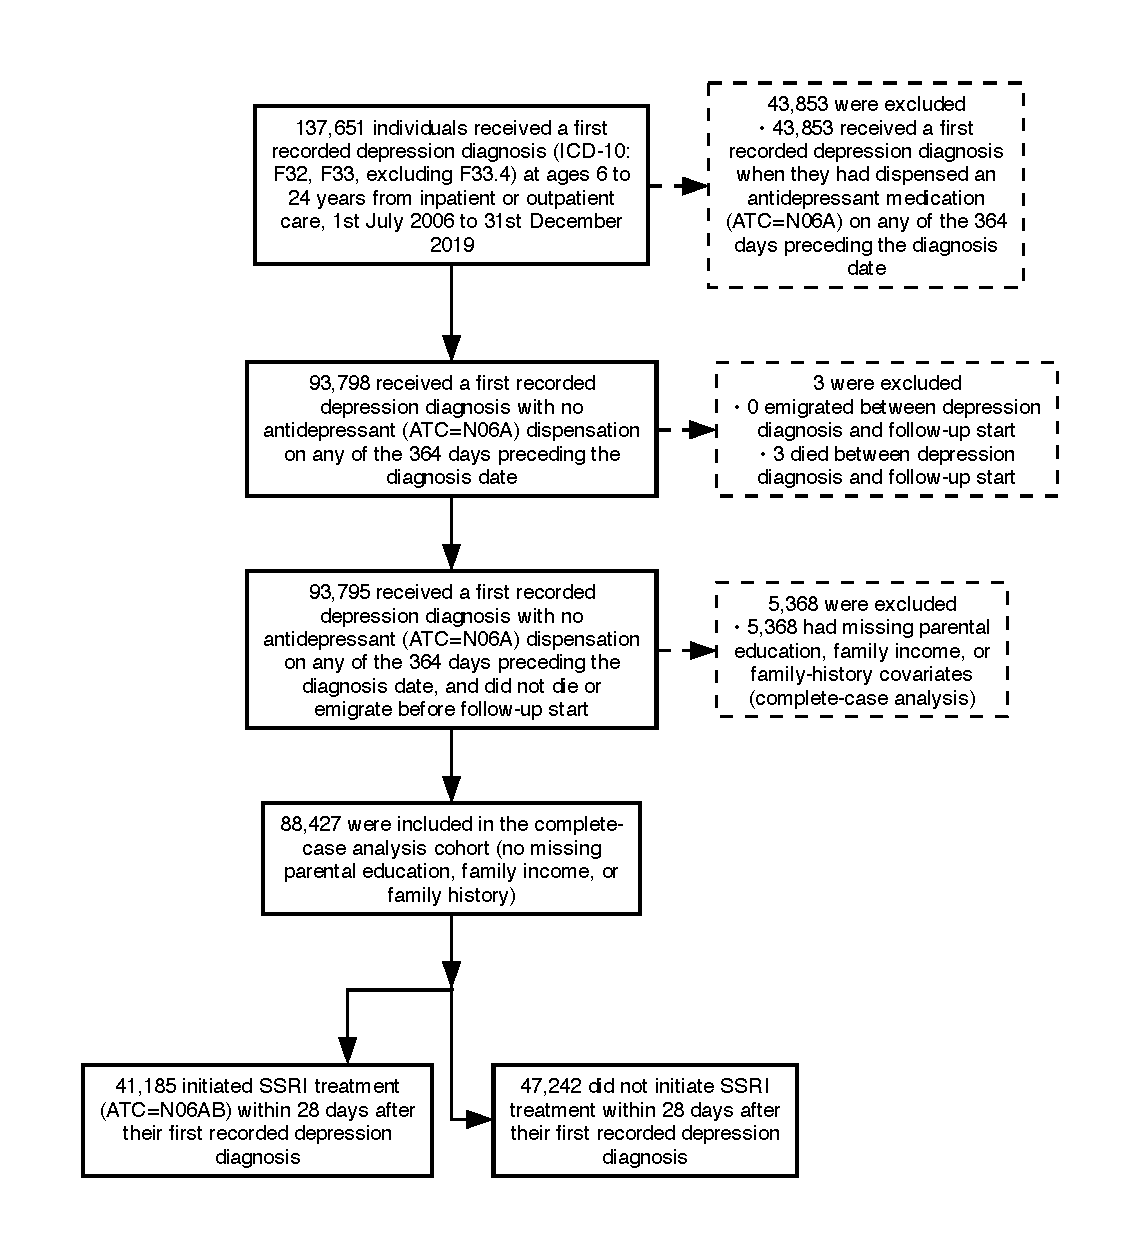
\includegraphics[width=1.00\textwidth]{figures/flowchart_cohort_inclusion_bw.pdf}
\caption{Flowchart of cohort inclusion criteria and study population derivation.}
\label{fig:flowchart}
\end{figure}

\subsection{Treatment definition}

SSRI initiators: Individuals who filled an SSRI prescription (ATC: N06AB) on the date of the depression diagnosis or any of the 28 days following it.

Non-initiators: Individuals who did not fill an SSRI prescription within 28 days.

The 28-day grace period allows for clinical assessment and treatment decisions following diagnosis \citep{lagerberg2023}. The empirical distribution of the diagnosis-to-first-dispensation lag among initiators is shown in Figure~\ref{fig:predi-diff} (Appendix~B).

\subsection{Outcome definition}

The primary outcome was suicidal behavior, defined as:
\begin{itemize}
    \item Intentional self-harm (ICD-10: X60--X84)
    \item Events of undetermined intent (ICD-10: Y10--Y34)
\end{itemize}

Events were identified from the NPR (inpatient and outpatient) and the Cause of Death Register.

\subsection{Follow-up}\label{sec:followup}

Follow-up began at the date of SSRI dispensation for initiators. For non-initiators, follow-up start was assigned using a frequency-matching approach to ensure comparable time-zero distributions, as in \citet{lagerberg2023}.

Follow-up ended at the earliest of:
\begin{itemize}
    \item Suicidal behavior event
    \item Death
    \item Emigration
    \item 12 weeks (84 days) after follow-up start
    \item Administrative end of study (December 31, 2020)
\end{itemize}

Events occurring on the same day as follow-up start were not counted as
outcomes.
The SSRI dispensation was treated as pre-exposure on day 0, so any
same-day suicidal-behavior event is interpreted as having preceded any
pharmacological effect of the drug.

\subsection{Covariates}

Baseline covariates used for confounding adjustment are listed in
Table~\ref{tab:covariates}. Diagnosis covariates were defined as any occurrence
in the NPR on or before the index date (follow-up start).
Medication covariates were defined as any dispensation in the 90 days up to and
including the index date. The mapping from the underlying register-code
variable names in the extraction pipeline to the thesis-facing labels used
throughout this report is given in Table~\ref{tab:varname-mapping} (Appendix~A).

{\setlength{\tabcolsep}{4pt}
\renewcommand{\arraystretch}{1.0}
\begin{longtable}{>{\hangindent=2em\hangafter=1}p{\dimexpr 0.45\textwidth-2\tabcolsep}p{\dimexpr 0.55\textwidth-2\tabcolsep}}
\caption{Baseline covariates used for confounding adjustment} \label{tab:covariates} \\
\toprule
\textbf{Variable} & \textbf{Description} \\
\midrule
\endfirsthead
\multicolumn{2}{l}{\itshape (Table~\ref{tab:covariates} continued)} \\
\toprule
\textbf{Variable} & \textbf{Description} \\
\midrule
\endhead
\midrule
\multicolumn{2}{r}{\itshape (continued on next page)} \\
\endfoot
\bottomrule
\endlastfoot
Calendar year & Year of index diagnosis (used in nuisance models only) \\
Care setting & Source of the index depression diagnosis in the NPR. Coded as O = outpatient, S = inpatient (``sluten v\aa rd''), or T = other/unknown source. For modelling, O and T are merged into a single non-inpatient category contrasted against S. \\
\addlinespace
\multicolumn{2}{l}{\textit{Demographics}} \\
\quad Sex & 0 = male, 1 = female \\
\quad Age & Continuous; categorized into 0 = 6--11, 1 = 12--17, 2 = 18--24 years for iCF analyses \\
\addlinespace
\multicolumn{2}{l}{\textit{Socioeconomic factors}} \\
\quad Parental education & Highest parental education level (0 = primary, 1 = secondary, 2 = post-secondary, 99 = missing) \\
\quad Family income & Family disposable income, categorized as 1 = negative, 2 = zero, 3 = 1st--20th percentile of positive income, 4 = 20th--80th percentile, 5 = $>$80th percentile, 99 = missing \\
\addlinespace
\multicolumn{2}{l}{\textit{Family history (parental, ICD-10)}} \\
\quad Suicidal behavior & X60--X84 (intentional self-harm), Y10--Y34 (undetermined intent); 0/1/2 = count of biological parents with at least one such code; 99 = missing parental linkage \\
\quad Depression & F32--F33; 0/1/2 = count of biological parents with at least one such code; 99 = missing parental linkage \\
\addlinespace
\multicolumn{2}{l}{\textit{Prior psychiatric diagnoses (ICD-10, binary)}} \\
\quad Alcohol use disorder & F10 \\
\quad Substance use disorder & F11--F19, excluding tobacco (F17) \\
\quad Psychotic disorder & F20--F29 (schizophrenia and other psychotic disorders) \\
\quad Bipolar disorder & F30--F31 \\
\quad Phobic anxiety disorder & F40.0--F40.2 (agoraphobia, social phobias, specific phobias) \\
\quad Other anxiety disorder & F41.0--F41.1 (panic disorder, generalized anxiety disorder) \\
\quad Obsessive-compulsive disorder & F42 \\
\quad Stress/adjustment disorder & F43 \\
\quad Anorexia nervosa & F50.0--F50.1 \\
\quad Bulimia nervosa & F50.2--F50.3 \\
\quad Sleep disorder & F51 (non-organic sleep disorders) \\
\quad Cluster B personality disorder & F60.2--F60.3 (dissocial and emotionally unstable personality disorders) \\
\quad Intellectual disability & F70--F79 \\
\quad Autism spectrum disorder & F84.0/.1/.5/.8/.9 \\
\quad ADHD & F90 (hyperkinetic disorder) \\
\quad Conduct disorder & F91 \\
\quad Overdose/poisoning & T36--T51, X40--X49 \\
\quad Prior suicidal behavior & X60--X84 (intentional self-harm), Y10--Y34 (undetermined intent) \\
\addlinespace
\multicolumn{2}{l}{\textit{Prior medications (ATC, within 90 days before baseline, binary)}} \\
\quad Antipsychotic & N05A, excluding lithium (N05AN) \\
\quad Hypnotic/sedative & N05C \\
\quad Benzodiazepine & N05BA \\
\quad Antiepileptic & N03A, excluding mood stabilizers (N03AG01, N03AX09, N03AF01) \\
\quad Mood stabilizer & N05AN (lithium), N03AG01 (valproate), N03AX09 (lamotrigine), N03AF01 (carbamazepine) \\
\quad Psychostimulant & N06B \\
\quad Opioid & N02A \\
\quad Addiction medication & N07B (nicotine, alcohol, or opioid dependence treatments) \\
\addlinespace
\multicolumn{2}{l}{\textit{Healthcare utilization (binary)}} \\
\quad Prior psychiatric hospitalization & Any inpatient psychiatric admission before baseline \\
\end{longtable}
}

\label{sec:covariates-complete-case}
Four of the curated categorical covariates (parental education, family income, family history of suicidal behavior, and family history of depression) had non-trivial fractions of missing values arising from incomplete registry coverage or missing parental linkages in the registers.
The patterns of missingness across these four variables are reported in
Table~\ref{tab:missingness-patterns} (Appendix~\ref{sec:missingness-patterns}).
We restricted the analysis cohort to complete cases for these four variables.
In total,
\cohortExcludedCCA{} patients (\cohortExcludedCCAPct\% of the post-washout, post-pre-fu eligible cohort)
were excluded due to missing at least one value.
Complete-case restriction was applied uniformly to the main intention-to-treat (ITT) analyses, the sensitivity analyses, and the iCF / hdiCF subgroup analyses, so all downstream estimates share the same cohort. Family income was treated as a factor with five levels (negative, zero, 1st--20th percentile, 20th--80th percentile, $>$80th percentile) in the propensity-score model, following Lagerberg et al.\ \cite{lagerberg2023}.
For the iCF/hdiCF analyses it was retained on its integer scale so the forest could split between any pair of consecutive levels.

\subsection{Statistical analysis}

\subsubsection{Intention-to-treat analysis}

We used inverse probability weighting (IPW) to estimate the intention-to-treat effect. Stabilized weights were computed as:

\begin{equation}
SW_i = \frac{P(A=a_i)}{P(A=a_i | L_i)}
\end{equation}

where $A$ is treatment assignment, $a_i$ is the observed treatment for individual $i$, and $L_i$ is the vector of baseline covariates.

The treatment probability $P(A=1|L)$ was estimated using logistic regression. Weights were truncated at the 99th percentile to reduce the influence of extreme weights.

The primary estimand was the 12-week risk difference in suicidal behavior comparing SSRI initiation to no SSRI initiation. Cumulative incidence at 12 weeks was estimated as $1 - \hat{S}(t)$, where $\hat{S}(t)$ is the weighted Kaplan-Meier survival function. Risk differences and risk ratios with 95\% confidence intervals were calculated.

\subsubsection{Sensitivity analyses}

Two pre-specified sensitivity analyses assess robustness of the main ITT estimate:

\begin{enumerate}
    \item Exclusion of inpatient diagnoses: The main ITT analysis was repeated
        on the cohort restricted to individuals whose index depression
        diagnosis was made in a non-inpatient setting (outpatient or
        other/unknown setting). Inpatient diagnoses are a
        small fraction of the cohort but capture a
        clinically heterogeneous group with substantially different baseline
        suicide risk compared to outpatient-only patients
        \citep{bostwick2000}, and the IPW model has more uncertainty
        for these patients.
        Comparing the restricted-cohort ITT estimate with the main estimate
        quantifies how much the main result depends on the inpatient
        subset.
    \item Grace period: To assess sensitivity to the 28-day grace-period choice
        on treatment-group assignment, we rebuilt the cohort end-to-end under a
        stricter 14-day grace period. Patients whose first SSRI dispensation
        fell within 14 days of diagnosis are initiators, and the rest are
        non-initiators. The non-initiator follow-up start is frequency-matched
        to the new 14-day initiator distribution (rather than the 28-day one),
        and the death/emigration eligibility filter spans 14 days rather than
        28.
    \item Missing-indicator method: To assess how much of the complete-case
        restriction (Section~\ref{sec:covariates-complete-case}) drives the
        headline result, we re-fit the ITT analysis on the full eligible
        cohort (N = \sensMissIndN) without dropping rows on the four
        partially-observed covariates. A single binary indicator
        (\texttt{any\_miss}) marks patients with sentinel-99 in at least one
        of parental education, family income, family history of suicidal
        behavior, or family history of depression, and was added as a
        covariate in the PS model. For every patient with
        \texttt{any\_miss}~=~1, all four covariates were set to their modal
        reference level (parental education = secondary; family income =
        20th--80th percentile; both family-history variables = 0), so the
        indicator behaves as a clean ``missing-stratum'' flag whose
        coefficient absorbs the entire contribution of those patients via
        the four affected covariates. All other modelling choices match the
        headline ITT analysis. Known biases of this method are discussed in
        Section~\ref{sec:limitations}.
\end{enumerate}

Heterogeneity across age, sex, and additional covariates is addressed separately in the data-driven HTE analysis described in Section~\ref{sec:hte-methods}.

\subsection{Heterogeneous treatment effect analysis}\label{sec:hte-methods}

To identify patient subgroups with differential treatment effects, we applied the iterative causal forest (iCF) algorithm \citep{wang2024icf}. This method extends standard causal forests \citep{athey2019grf} by iteratively refining subgroup definitions to improve stability and interpretability.

\subsubsection{Overview of iterative causal forests}

Causal forests are an ensemble machine learning method that estimates heterogeneous treatment effects by partitioning the covariate space into regions with different conditional average treatment effects (CATEs). The iCF algorithm improves upon standard causal forests through:

\begin{enumerate}
    \item Variable selection: An initial causal forest identifies variables with importance above the mean, reducing the feature space to the most relevant effect modifiers. Importance is the depth-weighted frequency with which each covariate is used as a split across the trees in the forest, with splits near the root counted more heavily than deeper splits.
    \item Iterative tree construction: Multiple causal forests are grown at each candidate tree depth. The best tree from each forest (minimizing the R-loss objective of \citet{nie2021rlearner}, as used by iCF \citep{wang2024icf}) is extracted.
    \item Plurality voting: Across iterations, the most frequently occurring tree structure is selected, ensuring stability of subgroup definitions.
    \item Synthetic tree construction: Split values are averaged across trees with matching structure to define final subgroup boundaries.
    \item Cross-validation: K-fold cross-validation is used to select the optimal tree depth, balancing model complexity and predictive performance.
\end{enumerate}

\subsubsection{Implementation}

The iCF analysis was conducted with the following specifications:
\begin{itemize}
    \item K-fold cross-validation: $K = \icfKFolds$ folds
    \item Trees per forest: \icfNTrees
    \item Iterations per depth: \icfNIterationsCV{} (cross-validation), \icfNIterationsFinal{} (final model)
    \item Candidate depths: 2, 3, 4, and 5
    \item P-value threshold for heterogeneity test: \icfPThreshold
\end{itemize}

Age was categorized into three clinically meaningful groups: children (6--11 years), adolescents (12--17 years), and young adults (18--24 years). Calendar year was included in the nuisance models (propensity score and outcome regression) for confounding adjustment but excluded from the causal forest splitting candidates, since year is a confounder (related to both treatment propensity and outcome trends) but not a plausible effect modifier.

The raw causal forest used for variable selection (step 1 of the iCF pipeline)
is grown without \texttt{grf}'s built-in hyperparameter tuner
(\texttt{tune.parameters = "none"}, with an explicit RNG seed). Diagnostics on
this cohort found that the auto-tuner's choice of hyperparameters
varied substantially across
random seeds. The CV-MSE landscape that the tuner navigates is flat (relative
range $\sim 10^{-4}$, well below within-fold noise), so the tuner picks
essentially at random among configurations of roughly equivalent CV fit. With
tuning enabled, the above-mean-VI variable-selection step retained between 4
and 14 variables across five seeds, with the most
extreme draws producing aggressive-shrinkage forests
in which
most candidate covariates received zero splits (Appendix~\ref{sec:tuner-instability}).
Disabling the auto-tuner and
using \texttt{grf}'s honest defaults removes this source of nondeterminism
without measurably degrading the downstream voted-tree results.

Prior to running iCF, a heterogeneity test was performed using the calibration test from the initial causal forest to assess whether there is evidence of treatment effect heterogeneity \citep{athey2019grf}.

Subgroup-specific conditional average treatment effects (CATEs) were estimated using inverse probability of treatment weighting within each identified subgroup. Confidence intervals were obtained via bootstrap resampling.

\subsubsection{Raw causal forest and individual-level predictions}

The initial causal forest grown in step 1 of the iCF pipeline (prior to variable selection and iterative refinement) also produces individual-level CATE predictions $\hat{\tau}(X_i)$ for each patient. These predictions are useful for evaluating the overall degree of treatment effect heterogeneity through calibration analysis, Qini curves, and the area under the targeting operator characteristic curve (AUTOC) \citep{sverdrup2025}. This provides a complementary perspective to the iCF subgroup analysis. Whereas iCF produces discrete, interpretable subgroups, the raw causal forest's continuous CATE predictions capture the full spectrum of heterogeneity.

To assess robustness of the individual-level CATE predictions, we additionally compared three CATE estimators on the same cohort: the causal forest, a doubly-robust learner, and a T-learner. Calibration plots for all three are reported in Figure~\ref{fig:calibration}.

\subsubsection{High-dimensional iCF (hdiCF)}

To assess whether the curated covariate set might miss relevant effect
modifiers buried in the full diagnosis history or prescription history, we
also applied the high-dimensional iterative causal forest (hdiCF) algorithm of
\cite{wang2025hdicf}. The hdiCF extends iCF by generating ordinal
frequency-encoded features from individual ICD-10 and ATC codes recorded before
baseline, allowing the algorithm to discover finer-grained effect modifiers
(e.g., specific diagnosis codes) that are not represented in the curated
covariate set.

This design differs from the original hdiCF specification in
\citet{wang2025hdicf}, where HD features replaced rather than supplemented
predefined covariates. Wang used 200 most-prevalent codes per data dimension
with no curated covariate set. We retained the curated covariates because
they encode clinical knowledge (aggregated diagnosis categories matched
to known suicide risk factors, family-history flags, and class-level
medication exposure) that purely code-based HD features would only
approximate. The trade-off is candidate redundancy: a curated flag such as
\texttt{diag\_alcohol} and the HD features \texttt{dx.inp.F10} /
\texttt{dx.out.F10} encode overlapping signal, which can split the iCF
iterations' best-tree votes between correlated candidates and depress each
one's plurality fraction. We accepted this redundancy on the assumption
that the curated and HD variants are complementary in granularity: the
curated set absorbs broad clinical categories while the HD set adds
setting-specific resolution and ordinal code-frequency information that the
curated flags collapse over --- and that the iCF voting procedure is
sufficiently robust to consolidate on whichever variant best captures
effect modification. The empirical outcome on this cohort is reported in
Section~\ref{sec:hdicf-subgroups}.

Three classes of high-dimensional (HD) features were generated:
\begin{itemize}
    \item Inpatient diagnosis codes (\texttt{dx.inp.*}): ICD-10 3-character codes recorded in an inpatient setting on or before the index date
    \item Outpatient diagnosis codes (\texttt{dx.out.*}): ICD-10 3-character codes recorded in an outpatient setting on or before the index date
    \item Prescription codes (\texttt{rx.*}): ATC 5-character (chemical-subgroup) codes dispensed in the 90 days up to and including the index date, excluding all antidepressants (ATC N06A); aligned with the curated medication covariates
\end{itemize}

Antidepressants (N06A) are excluded from the HD prescription feature set to
avoid treatment leakage. Since the exposure is itself an N06AB dispensation,
an inclusive 90-day window would make any N06A feature a near-perfect proxy
for treatment rather than a baseline effect modifier. The curated medication
covariate set already excludes N06A, so this filter keeps the two covariate
sets free of antidepressants.

Each HD feature was encoded ordinally using patient-level frequency quartiles per Wang 2025 (0 = no occurrence, 1 = once, 2 = sporadic [2 to 75th percentile], 3 = frequent [$>$75th percentile]). Codes with population prevalence below 1\% were excluded, and up to 200 codes per data dimension were retained. The realized feature counts for this cohort are reported in Section~\ref{sec:hdicf-subgroups}; the full per-dimension breakdown of generated HD features is given in Table~\ref{tab:hd-features} (Appendix~A).

Per Wang 2025 recommendations for hdiCF, two methodological modifications were applied relative to base iCF:
\begin{enumerate}
    \item Heterogeneity test skipped: Sparse HD features dilute the calibration test signal, so the test is bypassed.
    \item Top 10\% variable selection: The above-mean VI threshold used in base iCF is too permissive when many sparse features are present; instead, only the top 10\% of variables by importance are retained for growing the iCF.
\end{enumerate}

All other iCF parameters (K-fold CV, tree depths, iteration counts, plurality voting) were held identical to the base iCF analysis.

\subsection{Software}

All analyses were conducted in R version 4.5.1. The \texttt{survival} package was used for Kaplan-Meier estimation, and custom code was developed for IPW calculations. Causal forests were implemented using the \texttt{grf} package \citep{athey2019grf}. The iterative causal forest algorithm was implemented following the methodology of \cite{wang2024icf}. Source code for the extraction and analysis pipelines is available at \url{https://github.com/Sebelino/ssri-suicidality}. Results reported in this thesis correspond to the \href{https://github.com/Sebelino/ssri-suicidality/tree/thesis-submission}{\texttt{thesis-submission}} Git tag.
The full study can be reproduced end-to-end, including the compilation of this thesis report. Access to the Karolinska Institutet Tensor HPC cluster is a precondition for this.

\subsection{Ethical considerations}

The study was approved by the Swedish Ethical Review Authority
(Dnr: 2020-06540). All analyses were performed on pseudonymized data
delivered by Statistics Sweden and the National Board of Health and
Welfare to Karolinska Institutet. Individual consent was waived under
the Swedish ethical-review framework for register-based research, where
contacting the underlying population would be both infeasible and
disproportionate given that the data have already been collected for
administrative purposes. Source data are held on Karolinska Institutet's
secure Tensor cluster, and no direct or indirect identifiers appear in
this thesis or its supplementary tables.

The data are nevertheless sensitive in several respects.
The cohort consists of children, adolescents, and
young adults aged 6--24, a group whose capacity to consent is limited
even when consent is sought. Records include psychiatric diagnoses,
antidepressant dispensations, and suicidal-behavior events.
Family-history covariates are derived from each biological parent's own
register records. Third-party health data has been linked without any
opportunity for the parents to consent or object. The pseudonymization,
the secure-storage requirement, and the absence of any individual-level
publication or re-identification are the practical safeguards for
this kind of register-based research.

Aside from data protection, there are a couple of ethical
considerations worth flagging.
The headline finding is that there exists a sex difference in early-period
suicidal-behavior risk at SSRI initiation. This finding could in principle be
misused to delay or withhold treatment from female patients on grounds of
attributed harm. Section~\ref{sec:clinical-implications} frames the
finding as an additional axis of caution to be raised in a risk-benefit
discussion at SSRI initiation, not as a basis for differential prescribing.
This distinction matters because untreated depression itself carries
substantial morbidity and the absolute risk increase reported here is
small (roughly one additional suicidal-behavior event per hundred patients
treated over 12 weeks). The deeper iCF subgroups, which surface candidate
modifiers based on parental education and family income, could similarly be
misread as identifying ``high-risk'' subgroups based on socioeconomic
status. We frame these explicitly as exploratory and not reproducible
across iterations precisely to discourage that reading.

% ==============================================================================
\section{Results}
% ==============================================================================

\subsection{Study population}

The complete-case analysis cohort comprised \studyN{} individuals aged 6--24 with a first depression diagnosis between 2006 and 2019 (after excluding \cohortExcludedCCA{} patients with missing parental education, family income, or family history; see Figure~\ref{fig:flowchart}). Of these, \studyNInitiators{} (\studyPctInitiators\%) initiated SSRI treatment within 28 days of diagnosis, while \studyNNoninitiators{} (\studyPctNoninitiators\%) did not. The mean age was \studyMeanAge{} years (SD = \studySdAge), and \studyPctFemale\% were female.

During the 12-week follow-up period, there were \studyEvents{} suicidal behavior events (\studyEventRate\% event rate), with \studyEventsInitiators{} events among SSRI initiators and \studyEventsNoninitiators{} events among non-initiators.

\subsection{Baseline characteristics}

Table~\ref{tab:baseline} presents baseline characteristics by treatment group.

{\setlength{\tabcolsep}{4pt}
\renewcommand{\arraystretch}{0.95}
\begin{longtable}{lccc}
\caption[Baseline characteristics by treatment group, before IPW weighting]{Baseline characteristics by treatment group on the complete-case analysis cohort (N = \studyN, see Figure~\ref{fig:flowchart}), before IPW weighting. SMD = absolute standardized mean difference. Baseline characteristics of the \cohortExcludedCCA{} patients excluded by the complete-case restriction are reported in Table~\ref{tab:baseline-excluded}.} \label{tab:baseline} \\
\toprule
\textbf{Characteristic} & \textbf{SSRI Initiators} & \textbf{Non-initiators} & \textbf{SMD} \\
 & (N = \studyNInitiators) & (N = \studyNNoninitiators) & \\
\midrule
\endfirsthead
\multicolumn{4}{l}{\itshape (Table~\ref{tab:baseline} continued)} \\
\toprule
\textbf{Characteristic} & \textbf{SSRI Initiators} & \textbf{Non-initiators} & \textbf{SMD} \\
 & (N = \studyNInitiators) & (N = \studyNNoninitiators) & \\
\midrule
\endhead
\midrule
\multicolumn{4}{r}{\itshape (continued on next page)} \\
\endfoot
\bottomrule
\endlastfoot
% Auto-generated by Summary_statistics.R -- do not edit manually
% Generated: 2026-05-14 16:51:47.557685
\textit{Demographics} &  &  &  \\
\quad Female, n (\%) & 26,527 (64.4) & 28,203 (59.7) & 0.10 \\
\quad Age category (years) &  &  & 0.11 \\
\quad\quad 6--11 & 736 (1.8) & 1,552 (3.3) &  \\
\quad\quad 12--17 & 19,229 (46.7) & 20,690 (43.8) &  \\
\quad\quad 18--24 & 21,220 (51.5) & 25,000 (52.9) &  \\
\textit{Socioeconomic factors} &  &  &  \\
\quad Source of depression diagnosis &  &  & 0.12 \\
\quad\quad Outpatient & 37,840 (91.9) & 41,772 (88.4) &  \\
\quad\quad Inpatient & 3,240 (7.9) & 5,200 (11.0) &  \\
\quad\quad Other/unknown source & 105 (0.3) & 270 (0.6) &  \\
\quad Parental education &  &  & 0.08 \\
\quad\quad Primary & 1,900 (4.6) & 2,942 (6.2) &  \\
\quad\quad Secondary & 18,739 (45.5) & 21,939 (46.4) &  \\
\quad\quad Post-secondary & 20,546 (49.9) & 22,361 (47.3) &  \\
\quad Family income &  &  & 0.09 \\
\quad\quad Negative & 78 (0.2) & 89 (0.2) &  \\
\quad\quad Zero & 46 (0.1) & 91 (0.2) &  \\
\quad\quad 1st--20th percentile & 7,072 (17.2) & 9,553 (20.2) &  \\
\quad\quad 20th--80th percentile & 25,099 (60.9) & 28,551 (60.4) &  \\
\quad\quad $>$80th percentile & 8,890 (21.6) & 8,958 (19.0) &  \\
\textit{Family history (count of biological parents)} &  &  &  \\
\quad Suicidal behavior &  &  & 0.02 \\
\quad\quad Neither parent & 37,247 (90.4) & 42,386 (89.7) &  \\
\quad\quad One parent & 3,745 (9.1) & 4,602 (9.7) &  \\
\quad\quad Both parents & 193 (0.5) & 254 (0.5) &  \\
\quad Depression &  &  & 0.03 \\
\quad\quad Neither parent & 30,838 (74.9) & 34,837 (73.7) &  \\
\quad\quad One parent & 9,395 (22.8) & 11,181 (23.7) &  \\
\quad\quad Both parents & 952 (2.3) & 1,224 (2.6) &  \\
\textit{Prior psychiatric diagnoses} &  &  &  \\
\quad Suicidal behavior, n (\%) & 2,876 (7.0) & 4,663 (9.9) & 0.10 \\
\quad Overdose/poisoning, n (\%) & 2,151 (5.2) & 3,776 (8.0) & 0.11 \\
\quad Anxiety disorder (F40, F41), n (\%) & 4,052 (9.8) & 4,281 (9.1) & 0.03 \\
\quad Stress/adjustment disorder, n (\%) & 3,708 (9.0) & 5,362 (11.4) & 0.08 \\
\quad ADHD, n (\%) & 4,893 (11.9) & 7,239 (15.3) & 0.10 \\
\quad Substance use disorder, n (\%) & 1,454 (3.5) & 3,244 (6.9) & 0.15 \\
\quad Alcohol use disorder, n (\%) & 1,998 (4.9) & 3,222 (6.8) & 0.08 \\
\quad OCD, n (\%) & 1,229 (3.0) & 1,148 (2.4) & 0.03 \\
\quad Sleep disorder, n (\%) & 1,502 (3.6) & 1,880 (4.0) & 0.02 \\
\quad Anorexia nervosa, n (\%) & 1,138 (2.8) & 1,223 (2.6) & 0.01 \\
\quad Bulimia nervosa, n (\%) & 457 (1.1) & 381 (0.8) & 0.03 \\
\quad Autism spectrum disorder, n (\%) & 2,308 (5.6) & 2,463 (5.2) & 0.02 \\
\quad Conduct disorder, n (\%) & 672 (1.6) & 1,094 (2.3) & 0.05 \\
\quad Bipolar disorder, n (\%) & 289 (0.7) & 846 (1.8) & 0.10 \\
\quad Psychotic disorder, n (\%) & 400 (1.0) & 847 (1.8) & 0.07 \\
\quad Organic mental disorder, n (\%) & 0 (0.0) & 0 (0.0) & 0.00 \\
\quad Cluster B personality disorder, n (\%) & 259 (0.6) & 666 (1.4) & 0.08 \\
\quad Intellectual disability, n (\%) & 542 (1.3) & 635 (1.3) & 0.00 \\
\textit{Prior medications} &  &  &  \\
\quad Antipsychotic, n (\%) & 1,299 (3.2) & 1,489 (3.2) & 0.00 \\
\quad Hypnotic/sedative, n (\%) & 11,299 (27.4) & 6,939 (14.7) & 0.32 \\
\quad Benzodiazepine, n (\%) & 1,823 (4.4) & 856 (1.8) & 0.15 \\
\quad Psychostimulant, n (\%) & 2,368 (5.7) & 3,028 (6.4) & 0.03 \\
\quad Opioid, n (\%) & 645 (1.6) & 908 (1.9) & 0.03 \\
\quad Antiepileptic, n (\%) & 121 (0.3) & 194 (0.4) & 0.02 \\
\quad Mood stabilizer, n (\%) & 351 (0.9) & 980 (2.1) & 0.10 \\
\quad Addiction medication, n (\%) & 118 (0.3) & 99 (0.2) & 0.02 \\
\textit{Healthcare utilization} &  &  &  \\
\quad Psychiatric hospitalization, n (\%) & 8,007 (19.4) & 12,177 (25.8) & 0.15 \\
\textit{SSRI type (initiators only)} &  &  &  \\
\quad Sertraline, n (\%) & 18,751 (45.5) &  &  \\
\quad Fluoxetine, n (\%) & 13,703 (33.3) &  &  \\
\quad Escitalopram, n (\%) & 4,733 (11.5) &  &  \\
\quad Citalopram, n (\%) & 3,702 (9.0) &  &  \\
\quad Paroxetine, n (\%) & 284 (0.7) &  &  \\
\quad Fluvoxamine, n (\%) & 12 (0.0) &  &  \\

\end{longtable}
}

\subsection{Intention-to-treat analysis}

Figure~\ref{fig:itt-cuminc} presents the weighted cumulative incidence curves for suicidal behavior by treatment group in the intention-to-treat analysis. These curves are derived from weighted Kaplan-Meier estimates as $1 - \hat{S}(t)$.

\begin{figure}[H]
\centering
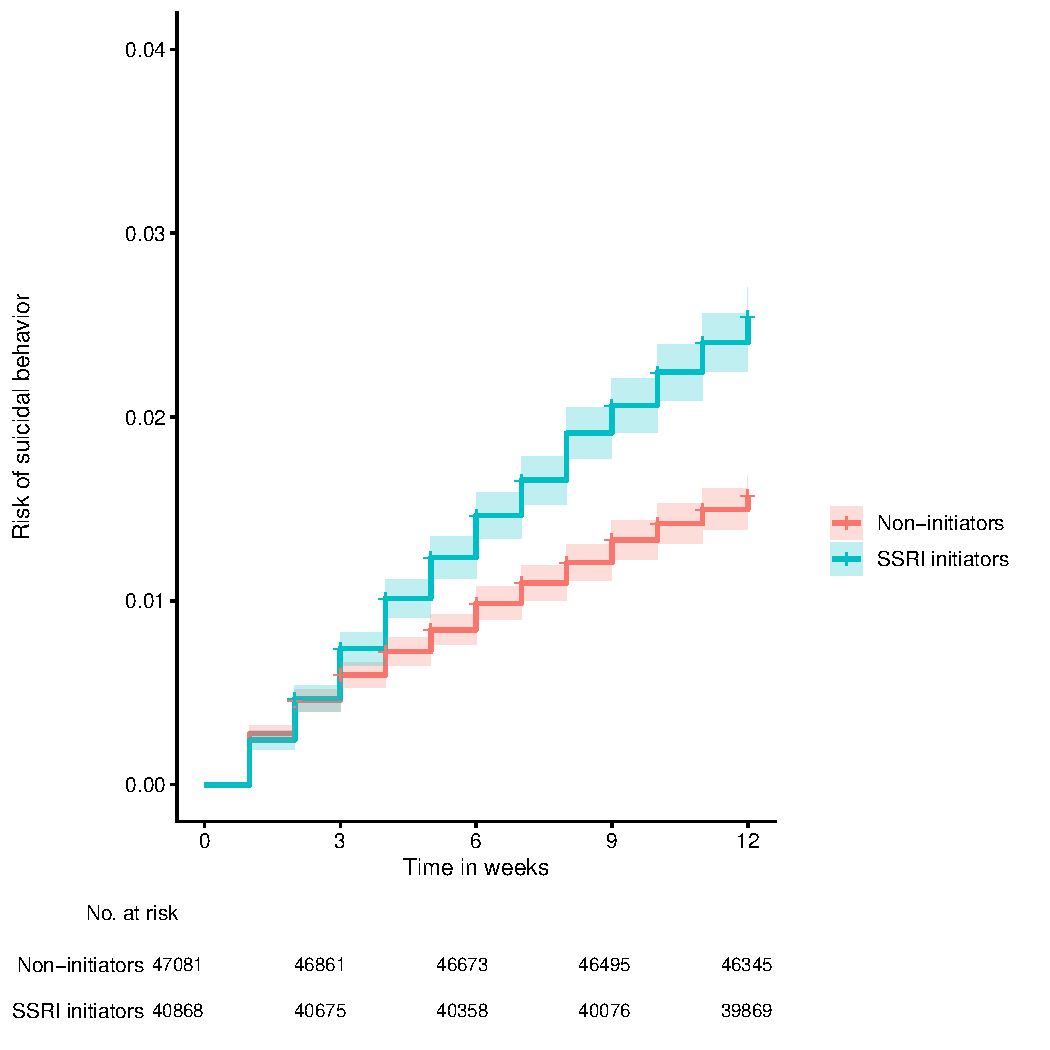
\includegraphics[width=0.9\textwidth]{figures/survplot_itt_main.pdf}
\caption[Weighted cumulative incidence curves for suicidal behavior by SSRI treatment status]{Weighted cumulative incidence curves for suicidal behavior by SSRI treatment status (intention-to-treat analysis), derived from Kaplan-Meier estimates. Shaded areas represent 95\% confidence intervals. At-risk counts in the panel below the curves are IPW-weighted (matching the weighted Kaplan--Meier estimator).}
\label{fig:itt-cuminc}
\end{figure}

Table~\ref{tab:itt-main} summarizes the 12-week intention-to-treat results,
including the raw patient counts in each arm. The at-risk panel beneath Figure~\ref{fig:itt-cuminc} reports IPTW-weighted counts and so falls a few hundred patients below these raw totals.

\begin{table}[H]
\centering
    \caption[Intention-to-treat analysis of SSRI initiation on 12-week suicidal behavior risk]{Intention-to-treat analysis of SSRI initiation on 12-week suicidal behavior risk. Risk = Adjusted 12-week cumulative incidence. RD = Adjusted risk difference in percentage points (pp). RR = Adjusted risk ratio. ``Adjusted'' = IPTW-weighted.}
\label{tab:itt-main}
\begin{tabular}{lrrrcc}
\toprule
 & \textbf{N} & \textbf{Events} & \textbf{Risk (\%)} & \textbf{RD (pp, 95\% CI)} & \textbf{RR (95\% CI)} \\
\midrule
SSRI initiators & \studyNInitiators & \studyEventsInitiators & \ittRiskTreated & \multirow{2}{*}{\ittRD{} (\ittRDLower, \ittRDUpper)} & \multirow{2}{*}{\ittRR{} (\ittRRLower, \ittRRUpper)} \\
Non-initiators & \studyNNoninitiators & \studyEventsNoninitiators & \ittRiskControl &  &  \\
\bottomrule
\end{tabular}
\end{table}

\subsection{Sensitivity analyses}

\subsubsection{Exclusion of inpatient diagnoses}

The main analysis was repeated on the cohort with inpatient index diagnoses excluded ($n = \sensExclInpTwelveN{}$). Table~\ref{tab:sens-excl-inp} compares the restricted-cohort estimate with the main full-cohort estimate.

\begin{table}[H]
\centering
\caption{Sensitivity analysis: ITT estimate with and without inpatient index diagnoses}
\label{tab:sens-excl-inp}
\begin{tabular}{lrrcc}
\toprule
\textbf{Cohort} & \textbf{N} & \textbf{Events} & \textbf{RD (pp, 95\% CI)} & \textbf{RR (95\% CI)} \\
\midrule
Main (full cohort)         & \studyN          & \studyEvents          & \ittRD{} (\ittRDLower, \ittRDUpper) & \ittRR{} (\ittRRLower, \ittRRUpper) \\
Excluding inpatients       & \sensExclInpTwelveN & \sensExclInpTwelveEvents & \sensExclInpTwelveRD{} (\sensExclInpTwelveRDLower, \sensExclInpTwelveRDUpper) & \sensExclInpTwelveRR{} (\sensExclInpTwelveRRLower, \sensExclInpTwelveRRUpper) \\
\bottomrule
\end{tabular}
\end{table}

Excluding inpatients yielded a slightly smaller absolute risk difference (RD shifted from \ittRD{} $\to$ \sensExclInpTwelveRD~pp) but a slightly larger risk ratio (RR \ittRR{} $\to$ \sensExclInpTwelveRR{}). Both estimates remain clearly significant and consistent in direction. The pattern is consistent with the lower baseline risk in the restricted cohort: removing the high-risk inpatient subset reduces the absolute scale of the contrast while the proportional effect of SSRI initiation is preserved. This indicates the headline finding is not driven by the inpatient subset.

\subsubsection{Grace period}

The 14-day rebuild reclassifies \cohortReclassFourteenRebuild{} patients (those
whose first dispensation fell in the (14, 28]-day window) from initiators to
non-initiators rather than excluding them. Of those,
\cohortReclassFourteenAnalysis{} remain in the complete-case analysis cohort.
After complete-case filtering, the 14-day cohort size is essentially identical
to the 28-day cohort (\sensGraceFourteenTwelveN{} vs.\ \studyN). The
single-patient discrepancy is a small-numbers artifact of re-running the
matching procedure, not a structural effect of the shorter grace window.
Under each rule, every non-initiator is assigned a baseline by random
sampling from the distribution of time-from-diagnosis-to-prescription among
initiators. Switching to the 14-day rule changes that distribution, so every
non-initiator's assigned baseline date changes. For one patient the new date
happens to fall on or after their death or emigration date, so they no longer
meet the requirement to be alive and resident in Sweden at baseline.
Table~\ref{tab:sens-grace14} compares the rebuilt 14-day analysis with the
main 28-day analysis.

\begin{table}[H]
\centering
\caption{Sensitivity analysis: ITT estimate under 28-day (main) and 14-day grace periods}
\label{tab:sens-grace14}
\begin{tabular}{lrrcc}
\toprule
\textbf{Grace period} & \textbf{N} & \textbf{Events} & \textbf{RD (pp, 95\% CI)} & \textbf{RR (95\% CI)} \\
\midrule
28 days (main) & \studyN & \studyEvents & \ittRD{} (\ittRDLower, \ittRDUpper) & \ittRR{} (\ittRRLower, \ittRRUpper) \\
14 days        & \sensGraceFourteenTwelveN & \sensGraceFourteenTwelveEvents & \sensGraceFourteenTwelveRD{} (\sensGraceFourteenTwelveRDLower, \sensGraceFourteenTwelveRDUpper) & \sensGraceFourteenTwelveRR{} (\sensGraceFourteenTwelveRRLower, \sensGraceFourteenTwelveRRUpper) \\
\bottomrule
\end{tabular}
\end{table}

The 14-day cutoff produced smaller estimates (RD \ittRD{} $\to$
\sensGraceFourteenTwelveRD~pp, RR \ittRR{} $\to$ \sensGraceFourteenTwelveRR{}).
Both estimates remain clearly significant and in the same direction. The
reduction reflects the \cohortReclassFourteenAnalysis{} reclassified patients
in the analysis cohort (initiators under the 28-day rule whose first SSRI
dispensation fell 15--28 days after diagnosis, and non-initiators under the 14-day
rule). They contributed events to the initiator group under the 28-day rule but
to the non-initiator group under the 14-day rule, mechanically diluting the
contrast when the grace window is shortened. Total events rise modestly
(\studyEvents{} $\to$ \sensGraceFourteenTwelveEvents) for a related reason:
under the 14-day rule the matching procedure draws non-initiator baselines
from a distribution capped at 14 days rather than 28, so the assigned
baselines are on average closer to the diagnosis date. Each non-initiator's
12-week follow-up window therefore shifts earlier and covers more of the
elevated suicidal-behavior risk in the weeks immediately after diagnosis. The headline
finding is robust in direction and remains clinically meaningful in magnitude
across grace-period specifications.

\subsubsection{Missing-indicator method}\label{sec:results-sens-missind}

To assess how much the complete-case restriction
(Section~\ref{sec:covariates-complete-case}) drives the headline result, we
re-fit the 12-week ITT analysis on the full eligible cohort
(N = \sensMissIndN, including the \cohortExcludedCCA{} patients excluded
under the complete-case rule). A single binary \texttt{any\_miss} indicator
(=1 for patients with sentinel-99 in at least one of the four
partially-observed covariates) was added to the PS model, and every patient
with \texttt{any\_miss}~=~1 was forced to the modal reference level on all
four covariates so the indicator coefficient absorbs the entire
missing-stratum contribution. Table~\ref{tab:sens-missind} compares the
missing-indicator estimate with the main complete-case estimate.

\begin{table}[H]
\centering
\caption{Sensitivity analysis: ITT estimate under the complete-case (main) and missing-indicator cohorts}
\label{tab:sens-missind}
\begin{tabular}{lrrcc}
\toprule
\textbf{Cohort policy} & \textbf{N} & \textbf{Events} & \textbf{RD (pp, 95\% CI)} & \textbf{RR (95\% CI)} \\
\midrule
Complete case (main)   & \studyN          & \studyEvents          & \ittRD{} (\ittRDLower, \ittRDUpper) & \ittRR{} (\ittRRLower, \ittRRUpper) \\
Missing indicator      & \sensMissIndN    & \sensMissIndEvents    & \sensMissIndRD{} (\sensMissIndRDLower, \sensMissIndRDUpper) & \sensMissIndRR{} (\sensMissIndRRLower, \sensMissIndRRUpper) \\
\bottomrule
\end{tabular}
\end{table}

Recovering the \cohortExcludedCCA{} patients dropped by the complete-case
rule barely shifted the estimate (RD \ittRD{} $\to$ \sensMissIndRD~pp, RR
\ittRR{} $\to$ \sensMissIndRR{}). This indicates the headline finding is not
driven by selection on observed missingness in the four partially-observed
covariates. The method's known biases (Section~\ref{sec:limitations}) mean
this should be read as a robustness check rather than an unbiased estimate on
the full cohort.

\subsection{Heterogeneous treatment effect analysis}

\subsubsection{Heterogeneity test}\label{sec:het-test}

The calibration test from the initial causal forest yielded a p-value of $\icfHetPvalue$, providing strong evidence of treatment effect heterogeneity across baseline covariates. This justified proceeding with the iterative causal forest algorithm to identify patient subgroups with differential treatment effects.

\subsubsection{Variable importance}

The initial causal forest identified \icfNSelectedVars{} variables with importance above the mean threshold, which were retained for subgroup identification. The top variables identified as potential effect modifiers were:
% Auto-generated by 04_export_latex.R -- do not edit manually
\begin{enumerate}
    \item Prior suicidal behavior diagnosis (importance: 0.127)
    \item Sex (importance: 0.110)
    \item Prior overdose/poisoning (importance: 0.103)
    \item Age group (importance: 0.097)
    \item Family income (importance: 0.081)
    \item Parental education level (importance: 0.074)
    \item Healthcare source (importance: 0.069)
    \item Alcohol use disorder (importance: 0.057)
    \item Prior psychiatric hospitalization (importance: 0.049)
    \item Family history of suicidal behavior (importance: 0.045)
    \item Hypnotic medication (importance: 0.043)
    \item Family history of depression (importance: 0.034)
\end{enumerate}


Figure~\ref{fig:icf-varimp} presents the variable importance scores for the top 20 covariates.

\begin{figure}[H]
\centering
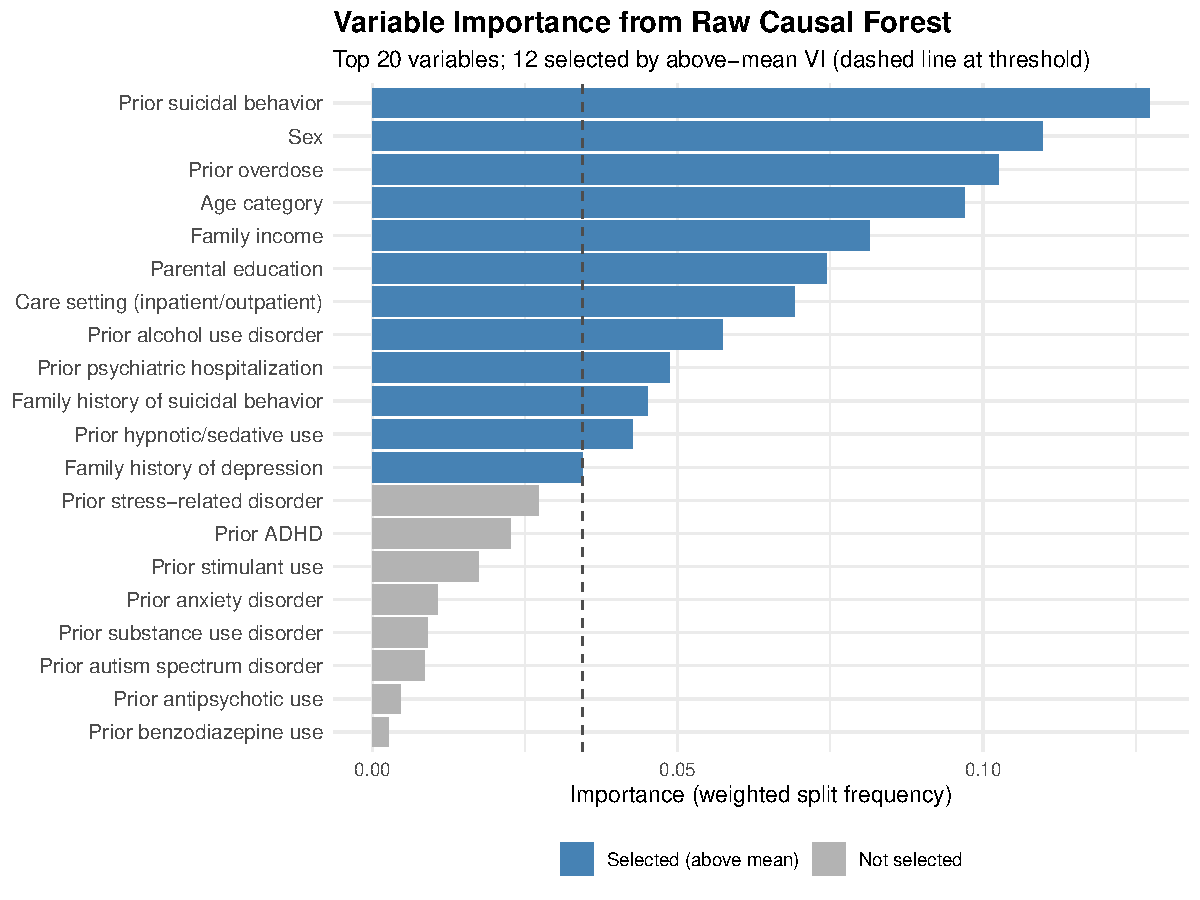
\includegraphics[width=0.9\textwidth]{figures/variable_importance.pdf}
\caption{Variable importance from the initial causal forest, showing the top 20 variables ranked by their contribution to treatment effect heterogeneity. Importance is measured as the weighted frequency of splits on each variable.}
\label{fig:icf-varimp}
\end{figure}

\subsubsection{Individual-level treatment effect heterogeneity}

Figure~\ref{fig:icf-cate-dist} shows the distribution of individual-level CATE
estimates from the initial (raw) causal forest, sorted from highest to lowest.
The majority of patients have small positive CATEs near the average treatment
effect. A minority on the left of the curve have substantially elevated
predicted risk increases following SSRI initiation. The dashed line indicates
the average treatment effect across the full cohort.

\begin{figure}[H]
\centering
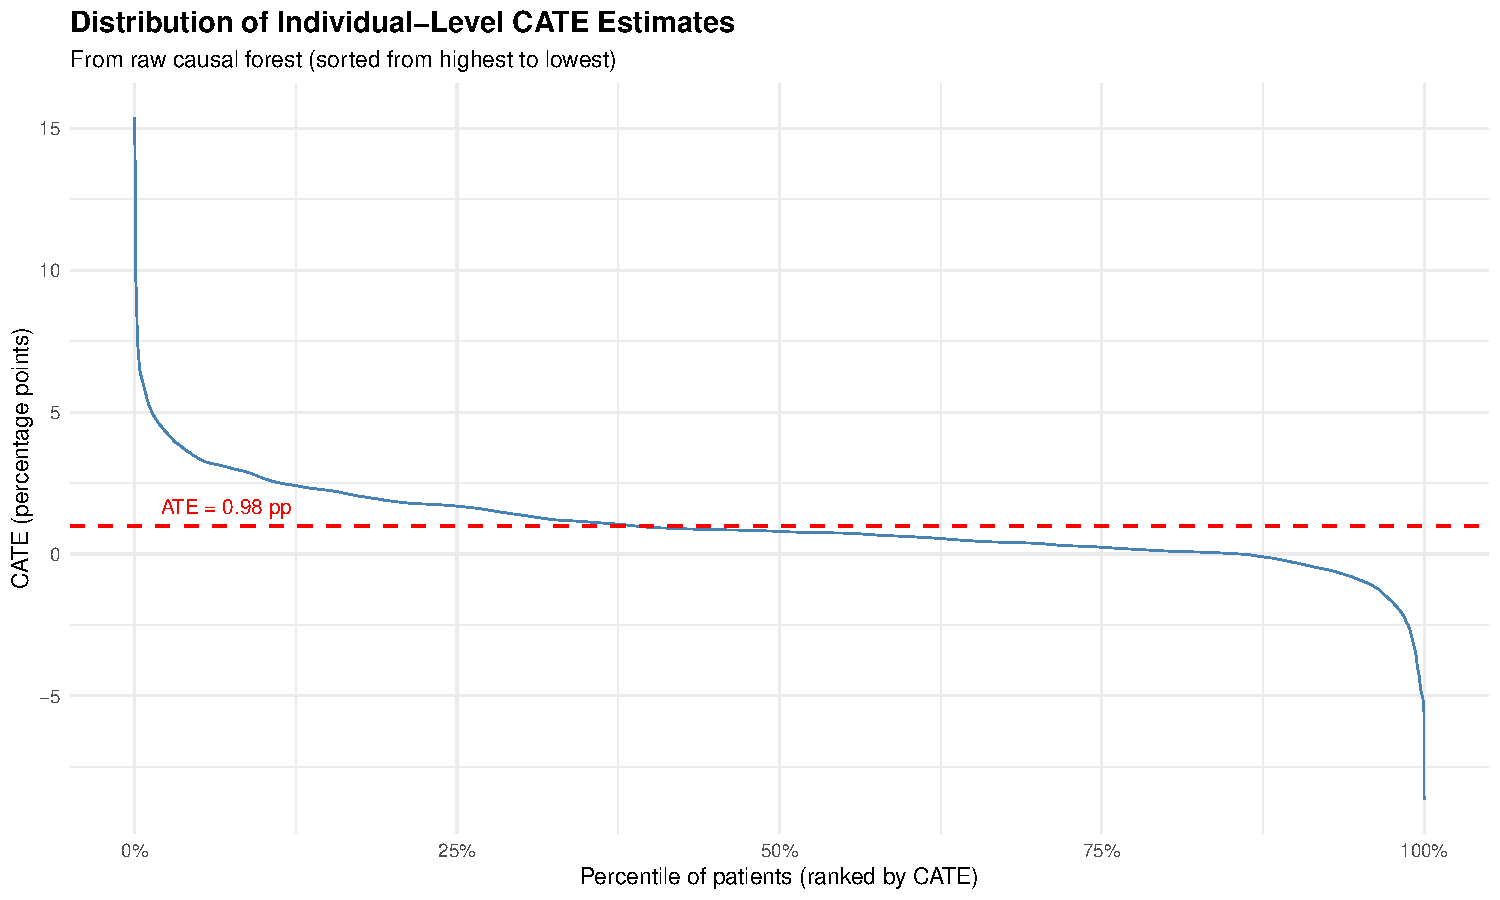
\includegraphics[width=0.9\textwidth]{figures/cate_distribution.pdf}
\caption{Distribution of individual-level conditional average treatment effect (CATE) estimates from the raw causal forest, sorted from highest to lowest. Each point represents one patient. The dashed line indicates the overall average treatment effect.}
\label{fig:icf-cate-dist}
\end{figure}

Figure~\ref{fig:icf-cate-hist} shows the same distribution as a histogram, with kernel density overlay, providing a complementary view of how the predicted CATEs are spread across the cohort.

\begin{figure}[H]
\centering
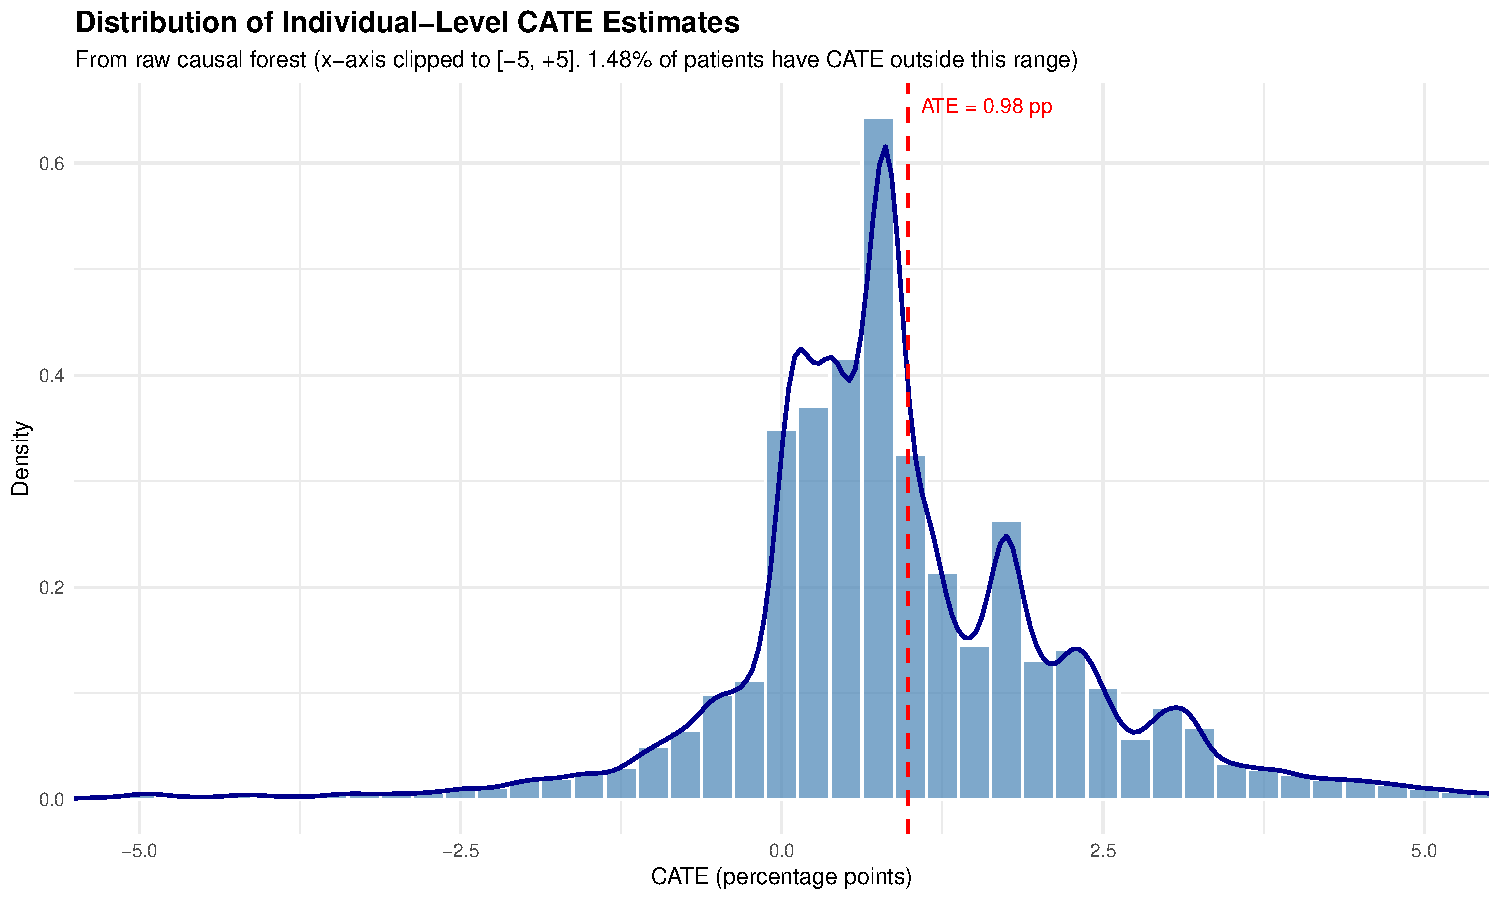
\includegraphics[width=0.9\textwidth]{figures/cate_distribution_histogram.pdf}
\caption{Histogram of individual-level CATE predictions from the raw causal forest, with kernel density overlay. The dashed line indicates the overall average treatment effect.}
\label{fig:icf-cate-hist}
\end{figure}

\subsubsection{CATE calibration}

To assess whether the causal forest's individual-level CATE predictions are well-calibrated, we binned patients into deciles of predicted CATE and compared the mean predicted effect with the IPTW-weighted observed treatment effect within each bin (Figure~\ref{fig:calibration}). A well-calibrated model produces points along the diagonal (predicted = observed). For comparison, we also computed calibration for two alternative CATE estimators on the same cohort: a doubly-robust learner (DR) and a T-learner.

Calibration is summarized by three statistics: the slope of the regression of observed bin-means on predicted bin-means (ideal = 1), the intercept (ideal = 0), and the mean absolute calibration error (MACE) across the ten bins. Table~\ref{tab:calibration} reports these statistics for the three estimators alongside the predicted and observed decile-mean ranges.

\begin{table}[H]
\centering
\caption[Calibration statistics for the three CATE estimators]{Calibration statistics for the three CATE estimators (causal forest, doubly-robust learner, T-learner). Slope, intercept, and R$^2$ are from the regression of observed bin-means on predicted bin-means (ideal slope = 1, intercept = 0, R$^2$ = 1). MACE = mean absolute calibration error in percentage points (ideal = 0). Predicted and observed ranges are the decile-mean min/max across the ten bins.}
\label{tab:calibration}
\setlength{\tabcolsep}{6pt}
\footnotesize
\begin{tabular}{lrrrrcc}
\toprule
\textbf{Estimator} & \textbf{Slope} & \textbf{Intercept} & \textbf{R$^2$} & \textbf{MACE (pp)} & \textbf{Predicted (pp)} & \textbf{Observed (pp)} \\
\midrule
Causal forest    & \calibCFSlope & \calibCFIntercept & \calibCFRsq & \calibCFMACE & \calibCFPredMin{} to \calibCFPredMax & \calibCFObsMin{} to \calibCFObsMax \\
Doubly-robust    & \calibDRSlope & \calibDRIntercept & \calibDRRsq & \calibDRMACE & \calibDRPredMin{} to \calibDRPredMax & \calibDRObsMin{} to \calibDRObsMax \\
T-learner        & \calibTLSlope & \calibTLIntercept & \calibTLRsq & \calibTLMACE & \calibTLPredMin{} to \calibTLPredMax & \calibTLObsMin{} to \calibTLObsMax \\
\bottomrule
\end{tabular}
\end{table}

The three estimators fail calibration in different ways. The causal forest has
the lowest MACE (\calibCFMACE~pp), but its slope of \calibCFSlope{} is well
below 1. Observed decile-means span only \calibCFObsMin{} to \calibCFObsMax~pp
around the cohort ATE while predicted decile-means range from \calibCFPredMin{}
to \calibCFPredMax~pp, so the CF overstates how much treatment effect varies
across the cohort.
For context, a trivial estimator that always predicts the cohort ATE
(\ittRD~pp) would have MACE roughly equal to the mean distance from the
observed deciles to the ATE -- well below \calibCFMACE~pp -- so the CF's MACE
is mostly explained by its mean tracking the ATE on average, not by capturing
heterogeneity. The T-learner has by far the best rank-ordering (R$^2$ =
\calibTLRsq) -- useful for ranking patients by treatment effect -- but its
observed decile range (\calibTLObsMin{} to \calibTLObsMax~pp) is implausibly
wide for the cohort-size and event-rate combination, suggesting
propensity-weight instability in tail deciles rather than informative
heterogeneity. The doubly-robust learner is nearly flat in slope
(\calibDRSlope) and poor in rank-ordering (R$^2$ = \calibDRRsq), reflecting the
high variance of its pseudo-outcomes in this cohort.


\begin{figure}[H]
\centering
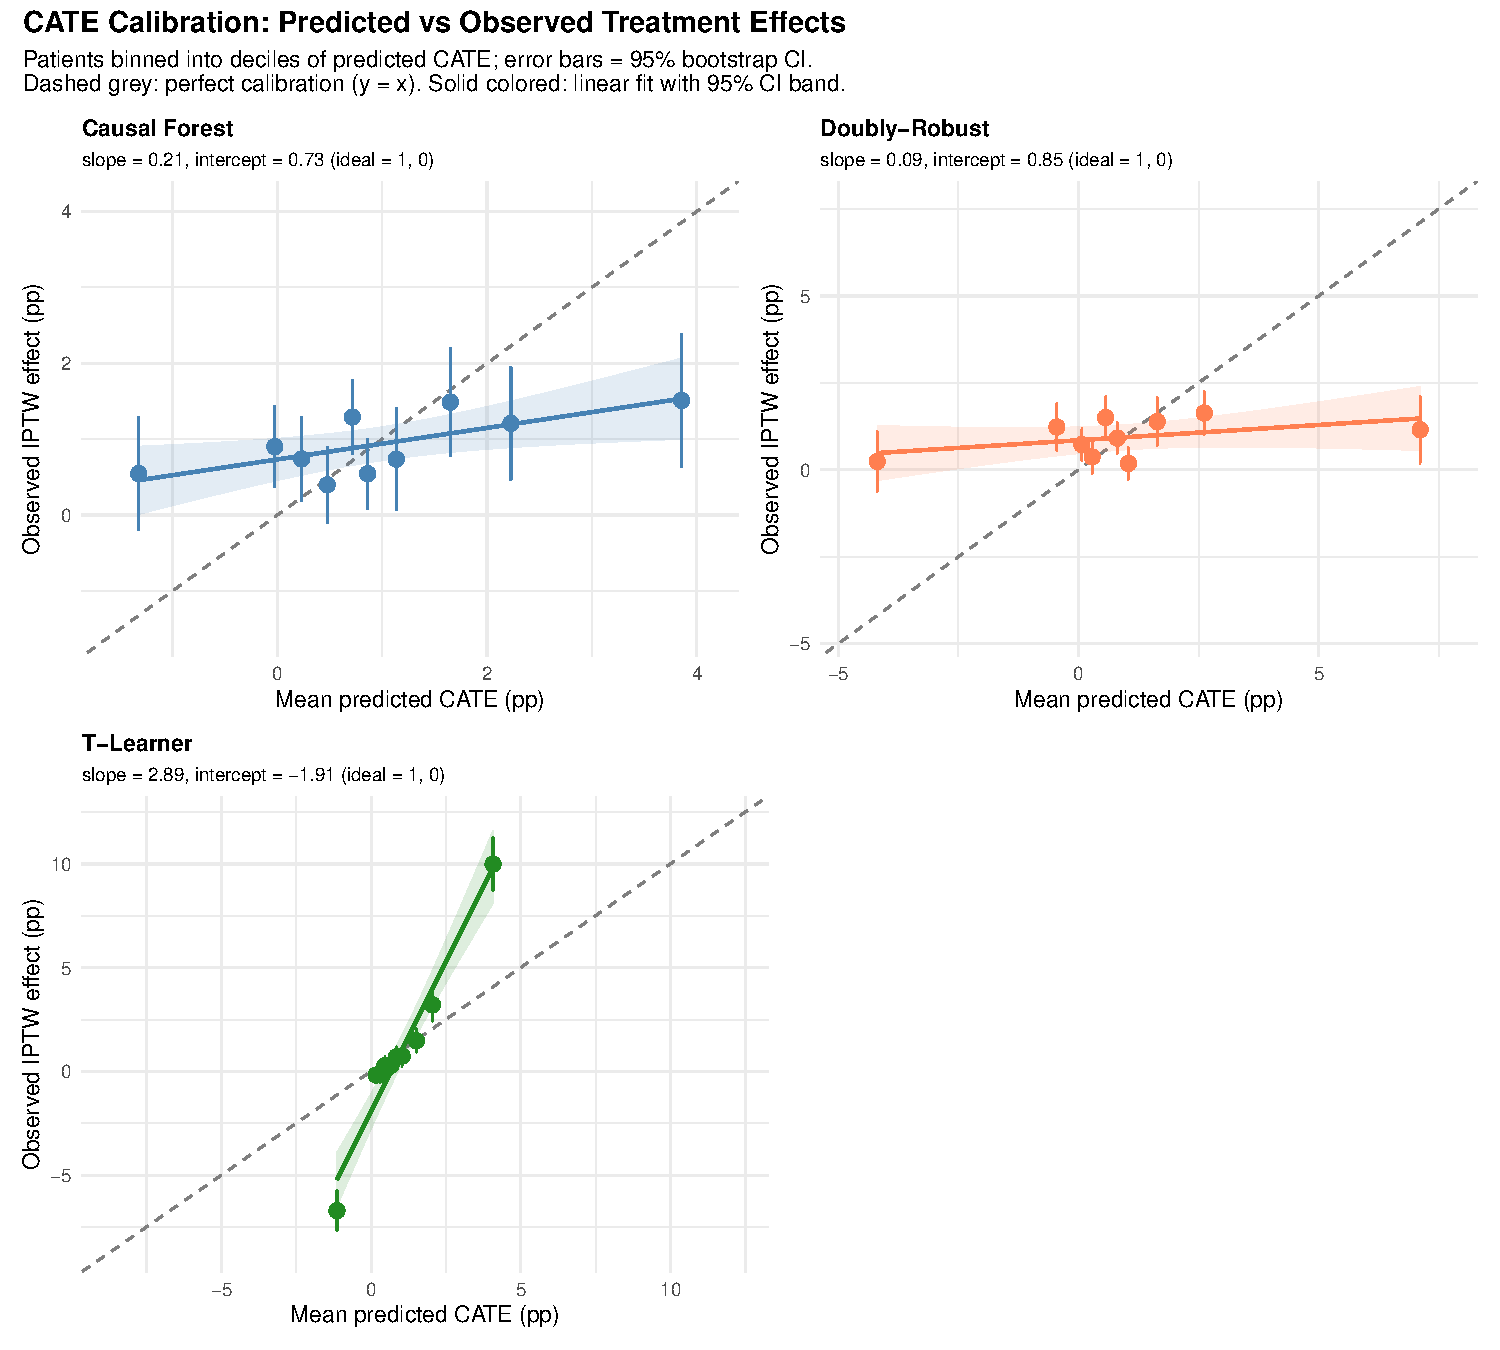
\includegraphics[width=\textwidth]{figures/calibration_plot.pdf}
\caption{CATE calibration plot. Patients are binned into deciles of predicted CATE; within each bin, the mean predicted CATE (x-axis) is compared to the IPTW-weighted observed treatment effect (y-axis). Error bars represent 95\% bootstrap confidence intervals. The dashed line indicates perfect calibration.}
\label{fig:calibration}
\end{figure}

\subsubsection{Subgroup identification}\label{sec:icf-subgroups}

Given the heterogeneity-test rejection (Section~\ref{sec:het-test}), we ran the iCF algorithm to identify the tree structure underlying it. The Wang 2024 iCF selects depth by cross-validated mean squared error (CV-MSE), growing iCFs at each candidate depth $D\in\{2,3,4,5\}$ and reporting the argmin. Table~\ref{tab:cv-depth} reports the per-depth CV-MSE, within-fold standard deviation, and the variables appearing in the voted tree at each depth.

\begin{table}[H]
\centering
\caption[Cross-validation MSE by tree depth]{Cross-validation MSE and within-fold standard deviation by candidate depth. The CV-argmin (depth~\protect\icfCVMinDepth) and the 1-SE-selected headline depth (depth~\protect\icfBestDepth) are both indicated. ``Splitting variables'' lists the variables appearing in the voted tree at that depth, in depth-of-appearance order (root first).}
\label{tab:cv-depth}
\begin{tabular}{rccc}
\toprule
\textbf{Depth} & \textbf{Mean CV MSE} & \textbf{Within-fold SD} & \textbf{Splitting variables} \\
\midrule
\textbf{2} & \icfDTwoMeanCVMse & \icfDTwoCVMseSD & Sex \\
3          & \icfDThreeMeanCVMse & \icfDThreeCVMseSD & Sex, age \\
\textbf{4} & \icfDFourMeanCVMse & \icfDFourCVMseSD & Sex, age, education \\
5          & \icfDFiveMeanCVMse & \icfDFiveCVMseSD & Age, sex, fh-depr, income, education \\
\bottomrule
\end{tabular}
\end{table}

The CV-argmin is depth~\icfCVMinDepth, but the CV-MSE landscape is flat: the
within-fold SD exceeds the across-depth range by roughly two orders of
magnitude, so the argmin is governed by simulation variance rather than
out-of-sample fit, and all four candidate depths sit inside the 1-SE band
around the minimum. By the 1-SE rule of \citet{breiman1984cart}, we report the
shallowest depth in the plateau, with deeper trees in
Section~\ref{sec:icf-per-depth-trees} as sensitivity. The rule selects
depth~\icfBestDepth{} (two subgroups).

Figure~\ref{fig:icf-tree} visualizes the headline depth-\icfBestDepth{} tree while
Table~\ref{tab:icf-subgroups} reports its per-subgroup characteristics and
treatment effects.

\begin{figure}[H]
\centering
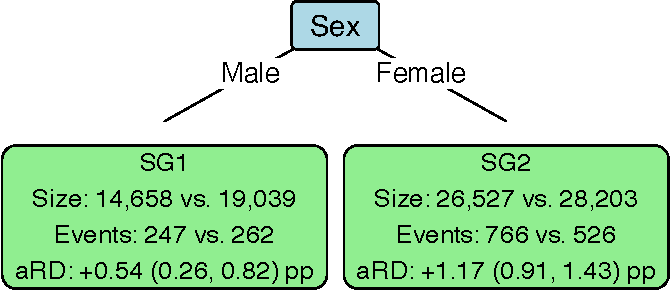
\includegraphics[width=0.6\textwidth]{figures/decision_tree_D2.pdf}
\caption{Headline iCF decision tree (depth~\protect\icfBestDepth{}, selected by the 1-SE rule). Decision nodes (blue) show the splitting variable and threshold; leaf nodes (green) show the identified subgroups with their CATE estimates in percentage points. Deeper voted trees are shown in Section~\protect\ref{sec:icf-per-depth-trees}.}
\label{fig:icf-tree}
\end{figure}

\begin{table}[H]
\centering
\caption[Subgroup-specific treatment effects identified by iterative causal forest]{Subgroup-specific treatment effects identified by iterative causal forest. CATE = conditional average treatment effect estimated using IPTW within each subgroup. Rates are events per 100 person-periods at 12 weeks.}
\label{tab:icf-subgroups}
\setlength{\tabcolsep}{4pt}
\footnotesize
\begin{tabular}{lrccc}
\toprule
\textbf{Subgroup} & \textbf{N} & \textbf{SSRI Rate (\%)} & \textbf{Control Rate (\%)} & \textbf{CATE (pp, 95\% CI)} \\
\midrule
% iCF subgroups
Male & 33{,}697 & 1.69 & 1.38 & +0.54 (0.26, 0.82) \\
Female & 54{,}730 & 2.89 & 1.87 & +1.17 (0.91, 1.43) \\
\bottomrule

\end{tabular}
\end{table}

The iCF CATE is \icfSGACATE~pp in males and \icfSGBCATE~pp in
females (roughly a \icfCATEratio$\times$ difference) and both subgroup
confidence intervals exclude zero.

\subsubsection{Stratified analysis: sex differences}

To validate the iCF subgroup findings, we conducted a stratified IPW analysis within each identified subgroup. Patients were assigned to iCF subgroups based on the synthetic decision tree, and the standard IPW-weighted Kaplan-Meier analysis (identical to the main ITT analysis) was run separately within each subgroup. Table~\ref{tab:icf-validation} compares the iCF CATE estimates with the independent stratified IPW risk differences.

\begin{table}[H]
\centering
\caption[Validation: iCF CATE vs.\ stratified IPW risk difference (RD)]{Validation: iCF CATE vs.\ stratified IPW risk difference (RD). iCF CATE uses IPTW with causal forest propensity scores. Stratified IPW RD uses IPW with logistic regression propensity scores (same method as the main ITT analysis). All values in percentage points.}
\label{tab:icf-validation}
\setlength{\tabcolsep}{4pt}
\footnotesize
\begin{tabular}{p{6cm}cc}
\toprule
\textbf{Subgroup} & \textbf{iCF CATE (95\% CI)} & \textbf{Stratified IPW RD (95\% CI)} \\
\midrule
Male   & \icfSGACATE{} (\icfSGACILower, \icfSGACIUpper) & \icfSGAStratIPW{} (\icfSGAStratIPWLower, \icfSGAStratIPWUpper) \\
Female & \icfSGBCATE{} (\icfSGBCILower, \icfSGBCIUpper) & \icfSGBStratIPW{} (\icfSGBStratIPWLower, \icfSGBStratIPWUpper) \\
\bottomrule
\end{tabular}
\end{table}

The two independent estimation approaches produce closely aligned point
estimates and confidence intervals. The iCF CATE and the stratified IPW RD
agree to within 0.1~pp in each subgroup, and both place the female effect at
roughly \icfCATEratio$\times$ the male effect. This suggests
that the headline subgroup contrast is not an artifact of the causal
forest methodology.

\subsubsection{Stratified analysis: prior suicidal behavior}\label{sec:strat-prior-suicidal}

Prior suicidal-behavior diagnosis ranked first in
the raw causal forest's variable importance
(Figure~\ref{fig:icf-varimp}: importance 0.127, ahead of sex at 0.110). Yet,
it did not appear in the voted tree at any candidate depth
(Table~\ref{tab:cv-depth}). To check whether this discrepancy hides a real
effect modifier that the plurality vote failed to converge on, we ran the
standard IPW-weighted ITT analysis. The analysis is identical to the main analysis, except
that the prior-suicidality covariate is dropped from the PS formula within each
stratum where it is constant. The analysis was done separately in the
\stratPriorSuicNoN{} patients without and the
\stratPriorSuicYesN{} patients with a prior suicidal-behavior diagnosis at
baseline. Table~\ref{tab:strat-prior-suicidal-risks} reports each
stratum's sample size, event count, and 12-week cumulative incidence by
treatment arm, and Table~\ref{tab:strat-prior-suicidal} the resulting risk
differences and risk ratios.

\begin{table}[H]
\centering
\caption{Per-stratum sample size, event count, and 12-week cumulative incidence of suicidal behavior by treatment arm (IPW-weighted Kaplan--Meier).}
\label{tab:strat-prior-suicidal-risks}
\begin{tabular}{lrrrr}
\toprule
\textbf{Stratum} & \textbf{N} & \textbf{Events} & \textbf{Non-initiators (\%)} & \textbf{Initiators (\%)} \\
\midrule
No prior suicidal behavior & \stratPriorSuicNoN  & \stratPriorSuicNoEvents  & \stratPriorSuicNoRiskControl  & \stratPriorSuicNoRiskTreated \\
Prior suicidal behavior    & \stratPriorSuicYesN & \stratPriorSuicYesEvents & \stratPriorSuicYesRiskControl & \stratPriorSuicYesRiskTreated \\
\bottomrule
\end{tabular}
\end{table}

\begin{table}[H]
\centering
\caption{ITT effect estimates stratified by prior suicidal-behavior diagnosis at baseline.}
\label{tab:strat-prior-suicidal}
\begin{tabular}{lcc}
\toprule
\textbf{Stratum} & \textbf{RD (pp, 95\% CI)} & \textbf{RR (95\% CI)} \\
\midrule
No prior suicidal behavior & \stratPriorSuicNoRD{} (\stratPriorSuicNoRDLower, \stratPriorSuicNoRDUpper)    & \stratPriorSuicNoRR{} (\stratPriorSuicNoRRLower, \stratPriorSuicNoRRUpper) \\
Prior suicidal behavior    & \stratPriorSuicYesRD{} (\stratPriorSuicYesRDLower, \stratPriorSuicYesRDUpper) & \stratPriorSuicYesRR{} (\stratPriorSuicYesRRLower, \stratPriorSuicYesRRUpper) \\
\bottomrule
\end{tabular}
\end{table}

The two strata show a familiar absolute-versus-relative split: patients with
a prior suicidal-behavior diagnosis have a higher baseline risk
(Table~\ref{tab:strat-prior-suicidal-risks}) and a numerically larger
absolute risk increase under SSRI initiation
(RD \stratPriorSuicYesRD{} vs.\ \stratPriorSuicNoRD~pp), but a smaller
relative risk (RR \stratPriorSuicYesRR{} vs.\ \stratPriorSuicNoRR{}). The
95\% CIs of the two RDs overlap, so the absolute-scale difference is not
itself statistically distinguishable.
This is discussed further in
Section~\ref{sec:discussion-prior-suicidal}.

\subsubsection{Per-depth decision trees}\label{sec:icf-per-depth-trees}

To examine what additional subgroup structure emerges at deeper tree depths
inside the 1-SE plateau, we grew iCF forests at each candidate depth and
extracted the voted decision tree with CATE estimates.
Figures~\ref{fig:tree-d2}--\ref{fig:tree-d5} show the voted trees at target
depths 2 through 5. ``Target depth'' is the \texttt{maxdepth} parameter passed
to \texttt{grf}. It is possible for the plurality vote across iCF iterations to
settle on a structure shallower than the target, in which case the rendered
tree is shallower than its caption's target value.
Depth~\icfBestDepth{}
(Figure~\ref{fig:tree-d2}) is the headline tree reported in
Section~\ref{sec:icf-subgroups}. Depth~\icfCVMinDepth{} is the CV-argmin
(Figure~\ref{fig:tree-d4}).
The cohort is complete-case for all categorical covariates,
so all ordinal splits are between legitimate covariate categories.

\begin{figure}[H]
\centering
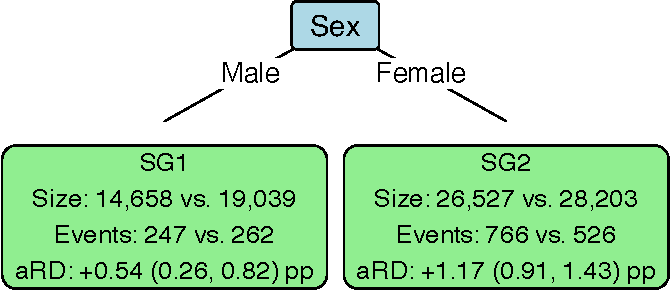
\includegraphics[width=0.6\textwidth]{figures/decision_tree_D2.pdf}
\caption{Voted iCF tree at target depth 2 (\protect\icfDTwoNSubgroups{} subgroups, voted-tree stability \protect\icfDTwoVoteFreq{}).}
\label{fig:tree-d2}
\end{figure}

\begin{figure}[H]
\centering
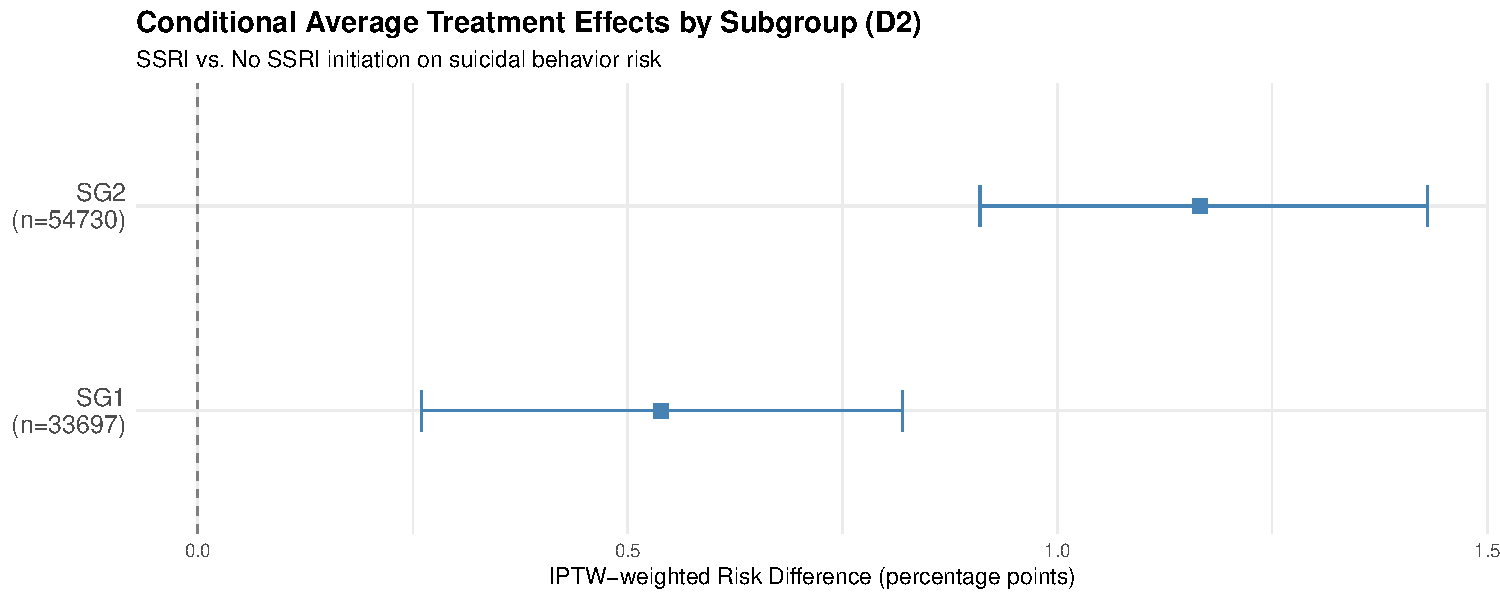
\includegraphics[width=0.9\textwidth]{figures/cate_forest_plot_D2.pdf}
\caption{Subgroup CATEs at target depth 2 (IPTW-weighted risk differences).}
\label{fig:cate-forest-d2}
\end{figure}

\begin{figure}[H]
\centering
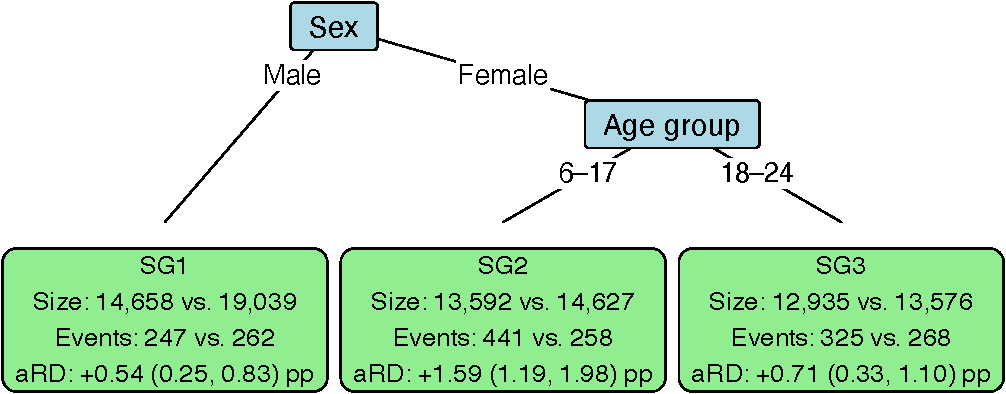
\includegraphics[width=\textwidth]{figures/decision_tree_D3.pdf}
\caption{Voted iCF tree at target depth 3 (\protect\icfDThreeNSubgroups{} subgroups, voted-tree stability \protect\icfDThreeVoteFreq{}).}
\label{fig:tree-d3}
\end{figure}

\begin{figure}[H]
\centering
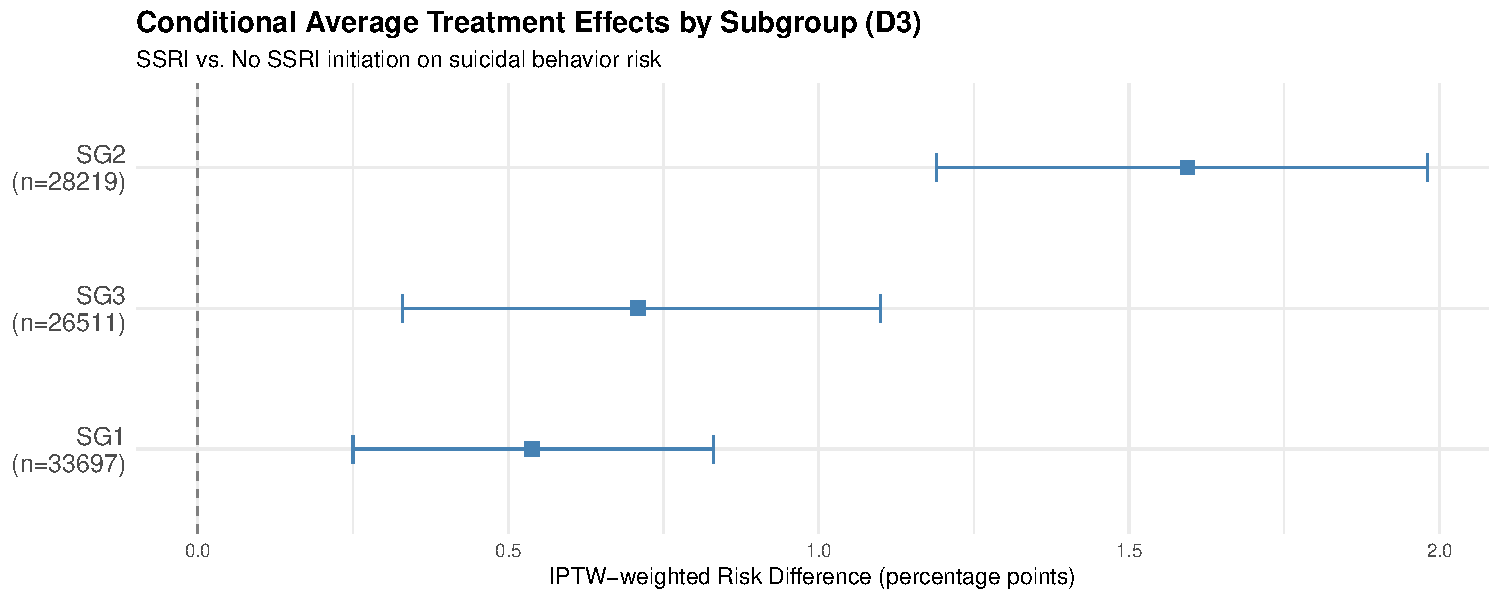
\includegraphics[width=0.9\textwidth]{figures/cate_forest_plot_D3.pdf}
\caption{Subgroup CATEs at target depth 3 (IPTW-weighted risk differences).}
\label{fig:cate-forest-d3}
\end{figure}

\begin{figure}[H]
\centering
\makebox[\textwidth][c]{%
  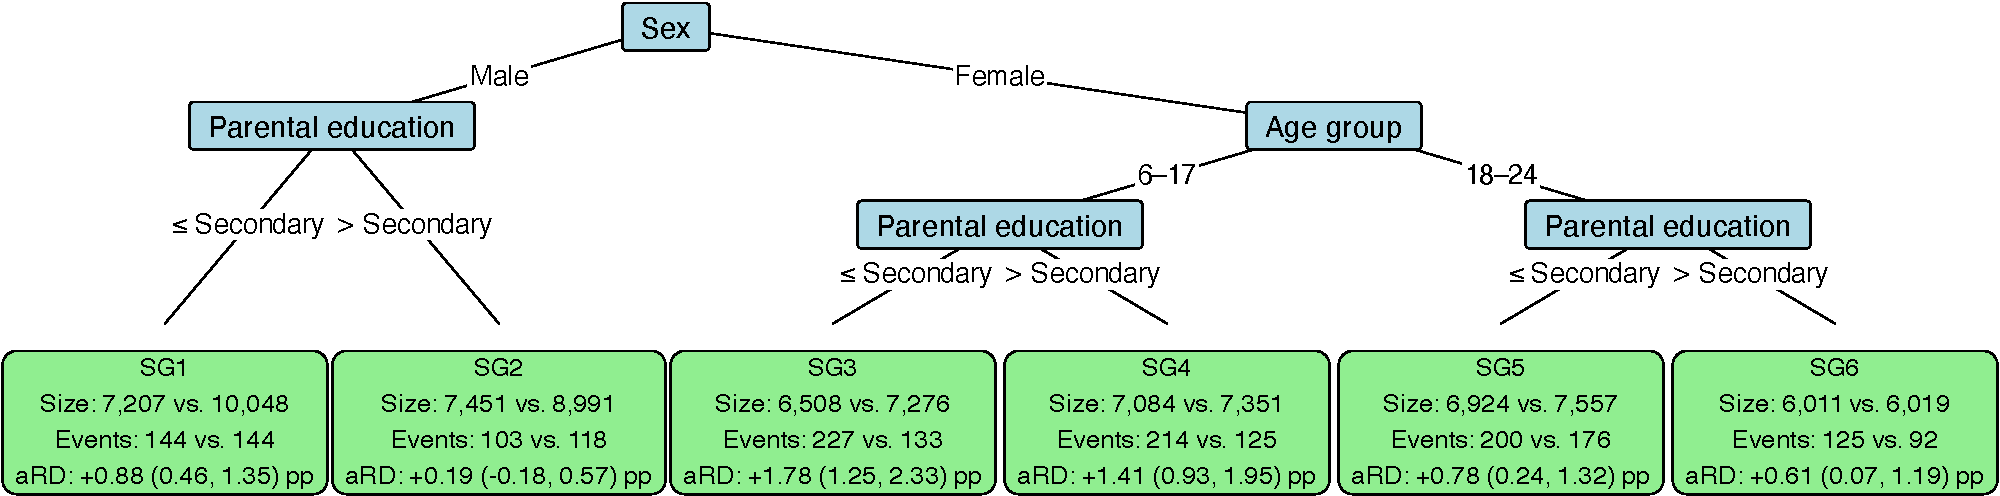
\includegraphics[width=1.2\textwidth]{figures/decision_tree_D4.pdf}%
}
\caption{Voted iCF tree at target depth 4 (\protect\icfDFourNSubgroups{} subgroups, voted-tree stability \protect\icfDFourVoteFreq{}).}
\label{fig:tree-d4}
\end{figure}

\begin{figure}[H]
\centering
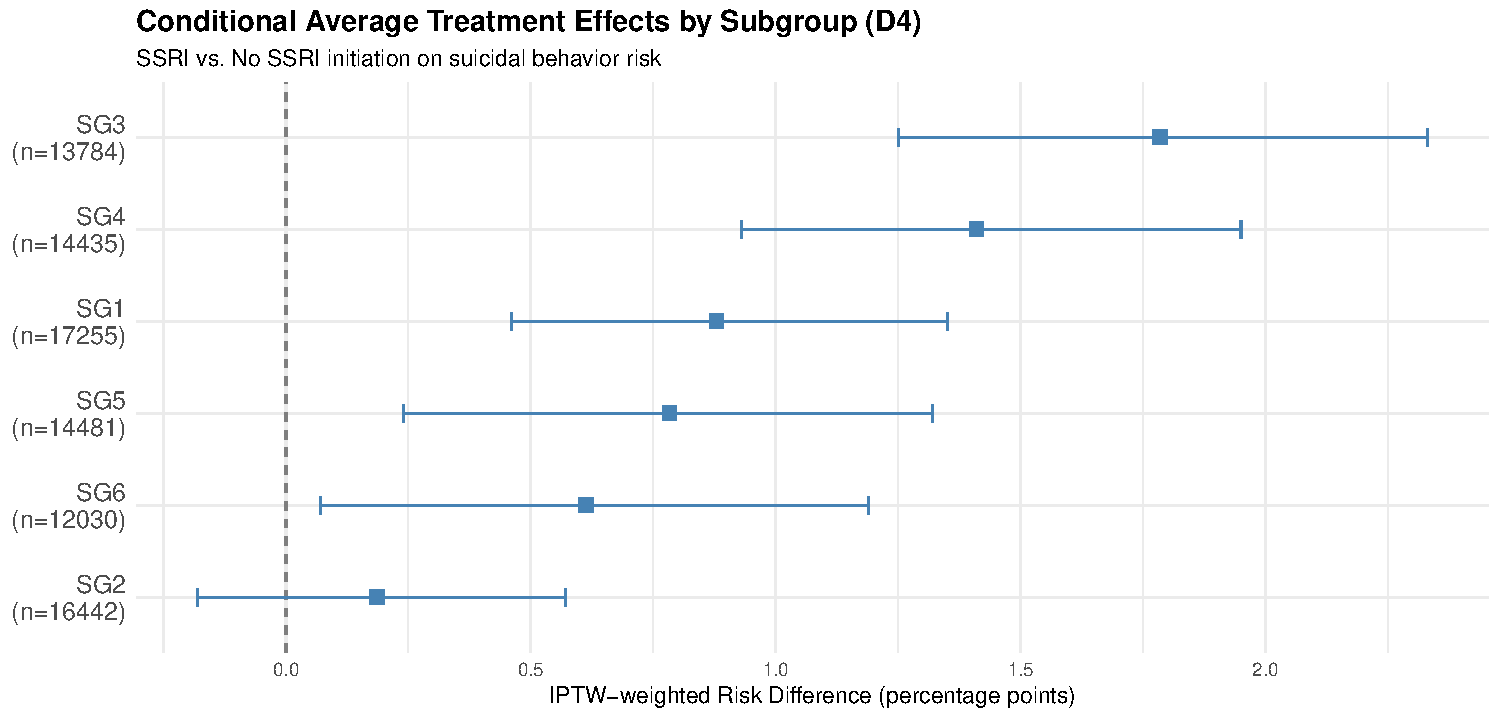
\includegraphics[width=0.9\textwidth]{figures/cate_forest_plot_D4.pdf}
\caption{Subgroup CATEs at target depth 4 (IPTW-weighted risk differences).}
\label{fig:cate-forest-d4}
\end{figure}

\begin{figure}[H]
\centering
\makebox[\textwidth][c]{%
  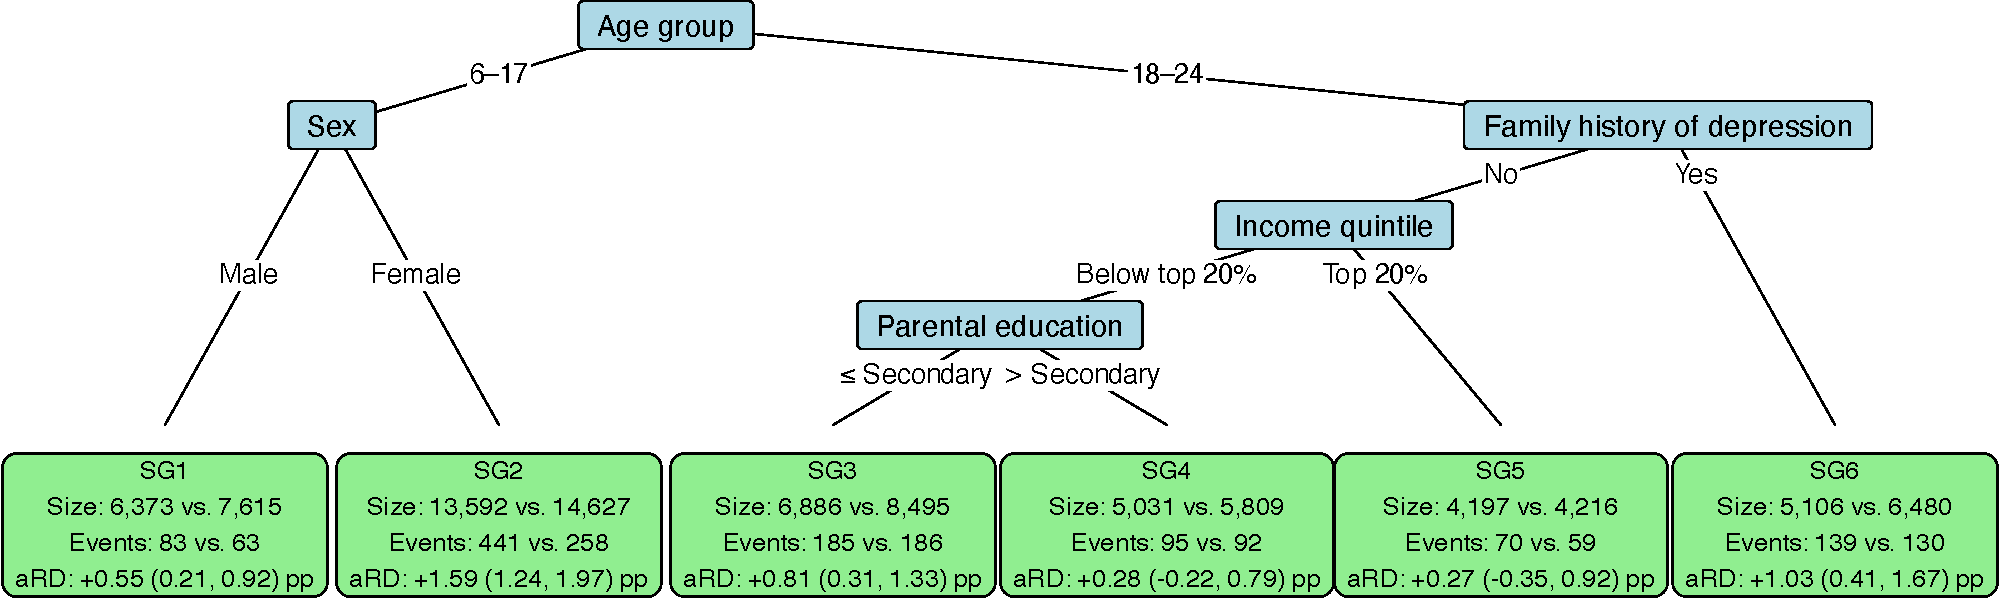
\includegraphics[width=1.2\textwidth]{figures/decision_tree_D5.pdf}%
}
\caption{Voted iCF tree at target depth 5 (\protect\icfDFiveNSubgroups{} subgroups, voted-tree stability \protect\icfDFiveVoteFreq{}).}
\label{fig:tree-d5}
\end{figure}

\begin{figure}[H]
\centering
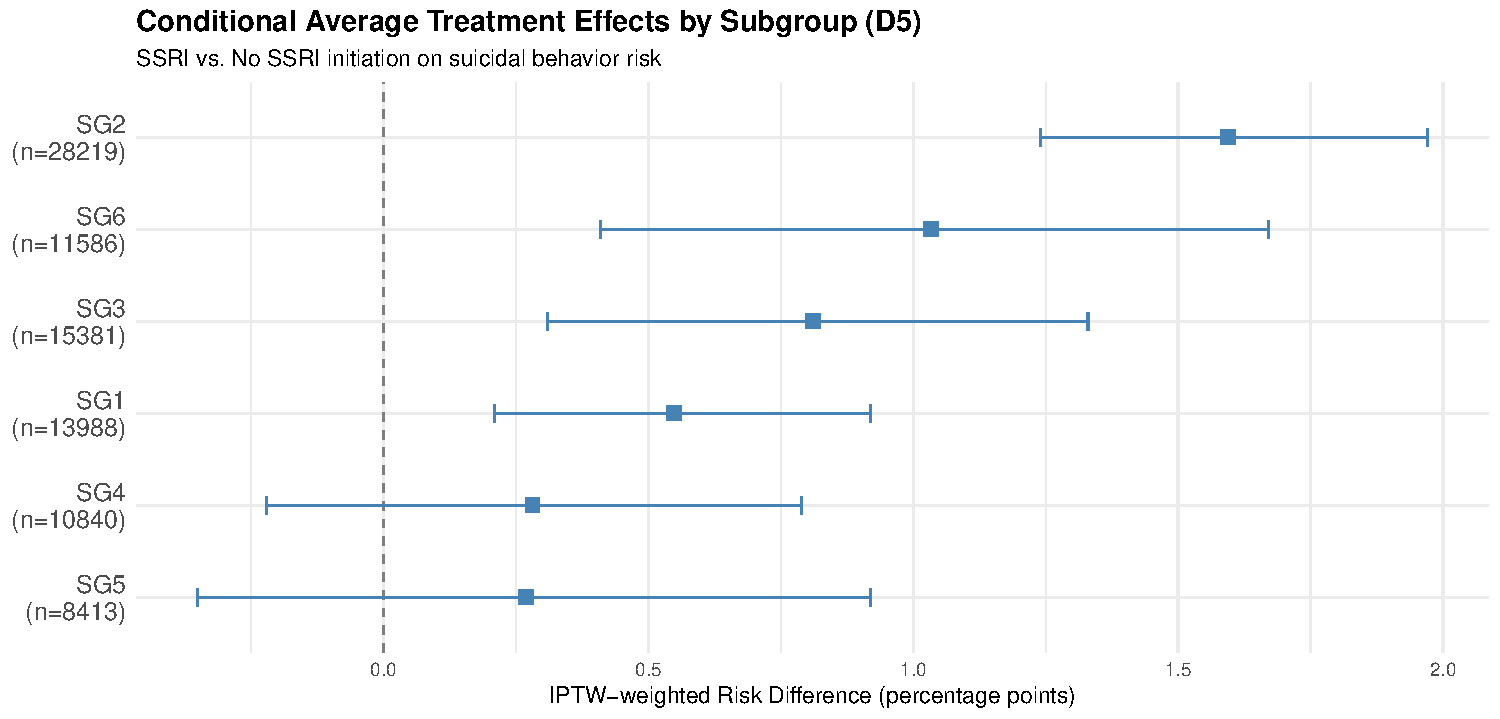
\includegraphics[width=0.9\textwidth]{figures/cate_forest_plot_D5.pdf}
\caption{Subgroup CATEs at target depth 5 (IPTW-weighted risk differences).}
\label{fig:cate-forest-d5}
\end{figure}

Figure~\ref{fig:tree-d5} shows the D5 leaf-level aRDs directly. Two of the six subgroups have CIs crossing zero, consistent with the D5 tree being underdetermined at this cohort size.

\subsubsection{Voted-tree structure distribution}\label{sec:icf-structure-dist}

The voted-tree stability summary in Section~\ref{sec:icf-per-depth-trees}
reports a single plurality fraction per depth. Figure~\ref{fig:structure-dist}
unpacks that fraction by showing the top-5 most-frequent tree structures across
iCF iterations at each candidate depth.
At depth~2 the algorithm picks a single structure
(\texttt{D1:Sex}) unanimously across all iterations.
Depth~3 narrows to
\icfDThreeNDistinctStruct{} close candidates with the top vote at
\icfDThreeVoteFreq{}. Depth~4 fragments across \icfDFourNDistinctStruct{}
distinct structures with the top vote falling to \icfDFourVoteFreq{}.
Depth~5
partially recovers (\icfDFiveNDistinctStruct{} structures, top vote
\icfDFiveVoteFreq) on an age-rooted tree that no longer matches the D2 sex
split.

\begin{figure}[H]
\centering
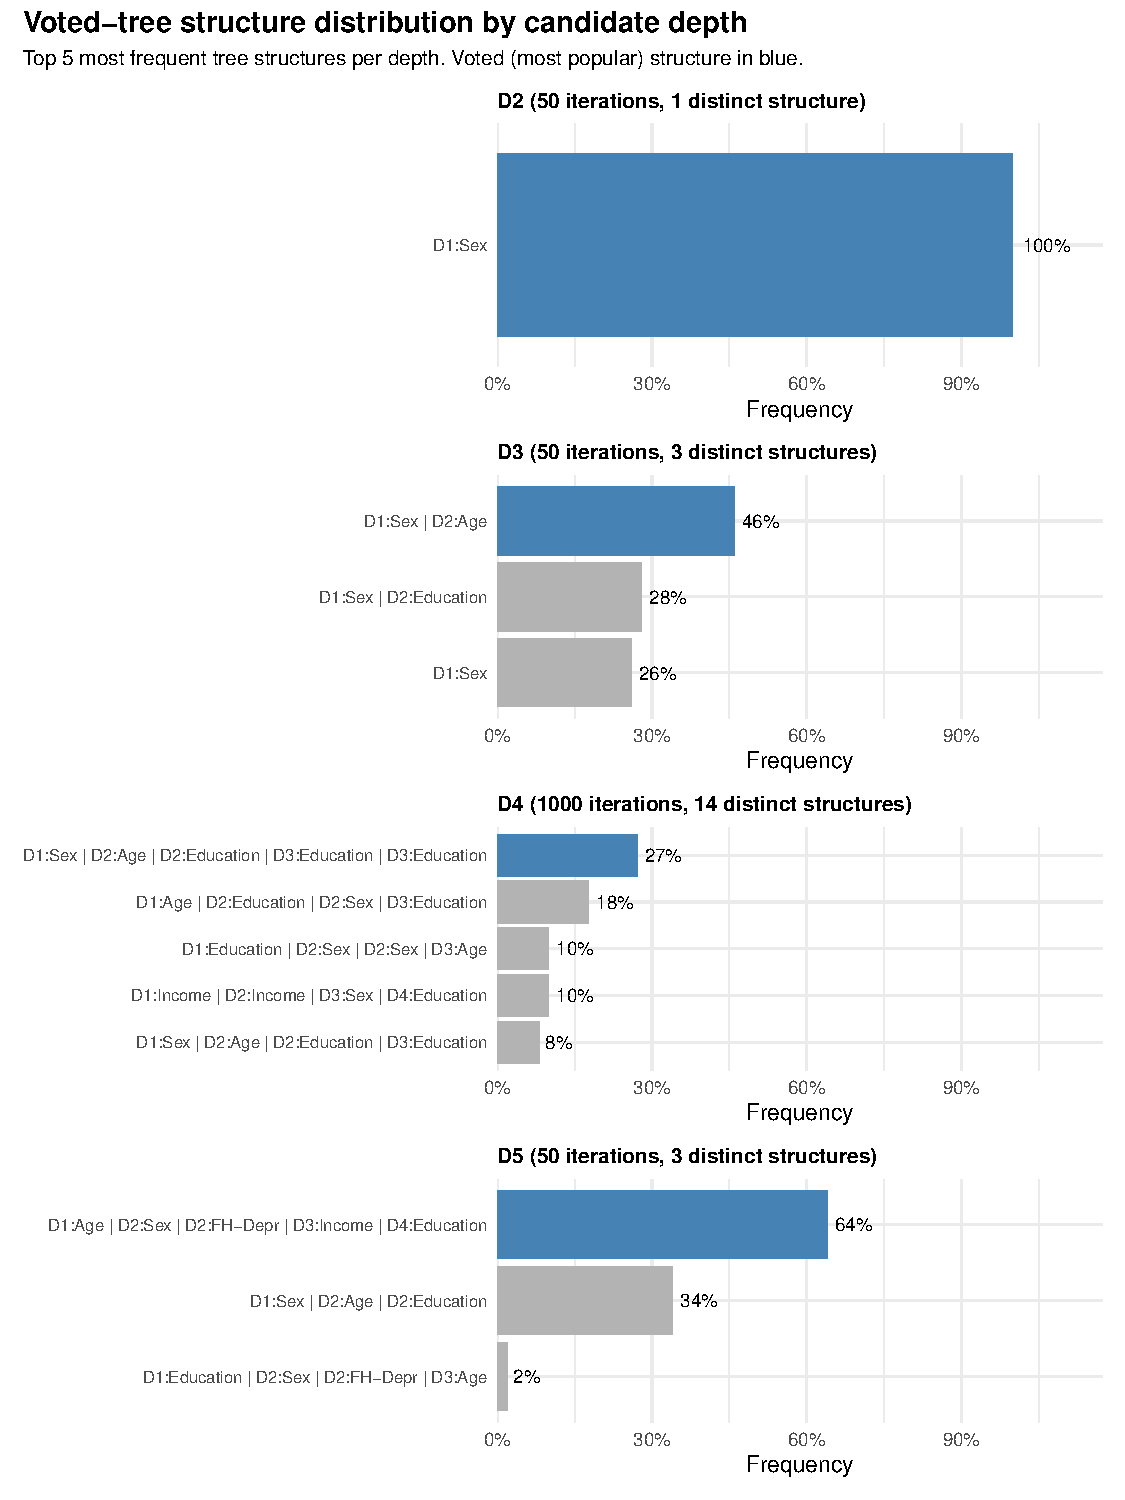
\includegraphics[width=0.95\textwidth]{figures/structure_distribution.pdf}
\caption{Voted-tree structure distribution across iCF iterations at each candidate depth. Each row in a panel is a distinct tree structure encoded as a pipe-separated list of depth-indexed split variables. Bar length is the fraction of iCF iterations that converged on that structure. The voted (top-plurality) structure is shown in blue. D4 uses 1{,}000 iterations (the headline-detection budget). D2/D3/D5 use 50 iterations each (the sensitivity budget).}
\label{fig:structure-dist}
\end{figure}

The shape of Figure~\ref{fig:structure-dist} is the structural counterpart of
the flat CV-MSE plateau in Table~\ref{tab:cv-depth}: when the candidate depth
is shallow enough to be identified by the data, the iCF iterations converge on
a single tree. When it is deeper than the data supports, they scatter across
many roughly-equivalent partitions.

Notably, the frequency of the most commonly selected tree falls sharply with
depth but recovers partially at D5.
D5's recovery is on a different structure where the first split is on age
and sex drops to depth 2.
This is a depth-dependent re-ordering
rather than a contradiction, and consistent with
\citet{wang2025hdicf}'s observation that deeper voted trees can settle on
different structures than their shallow counterparts.

\subsubsection{High-dimensional iCF (hdiCF)}\label{sec:hdicf-subgroups}

To probe for effect modifiers beyond the curated covariate set, we ran the
hdiCF pipeline with \hdicfNHDFeatures{} automatically generated HD features
(\hdicfNHDInp{} inpatient diagnoses, \hdicfNHDOut{} outpatient diagnoses,
\hdicfNHDRx{} prescriptions) alongside the curated variables. Per Wang 2025,
the calibration-based heterogeneity test was bypassed (the sparse ordinal HD
features dilute its signal), and the pipeline proceeded directly to variable
selection and subgroup identification. The CV-MSE landscape across candidate
depths was flat (relative range $\sim 10^{-4}$, far below the within-fold SD of
$\sim 10^{-2}$), so all four depths fell inside the 1-SE band. Applying the
same 1-SE rule used for base iCF (Section~\ref{sec:icf-subgroups}), the
headline depth is depth~\hdicfBestDepth{} (\hdicfNSubgroups{} subgroups: male
and female), with voted-tree stability \hdicfVoteFrequency. The Wang-2024
CV-argmin would have selected depth~\hdicfCVMinDepth{}. That deeper tree is
presented as a sensitivity in Section~\ref{sec:hdicf-per-depth-trees}. Of the
\hdicfNSelectedVars{} variables retained by the top-10\% importance filter, one
was an HD feature: inpatient depressive episode (\texttt{dx.inp.F32}).

The \hdicfNSelectedVars{} retained variables, in descending importance, are:
% Auto-generated by 05_export_latex.R -- do not edit manually
\begin{enumerate}
    \item Prior suicidal behavior (importance: 0.106)
    \item Prior overdose/poisoning (importance: 0.086)
    \item Family income (importance: 0.073)
    \item Parental education (importance: 0.065)
    \item Inpatient: F32 (importance: 0.062)
    \item Sex (importance: 0.058)
    \item Age group (importance: 0.054)
\end{enumerate}


\begin{figure}[H]
\centering
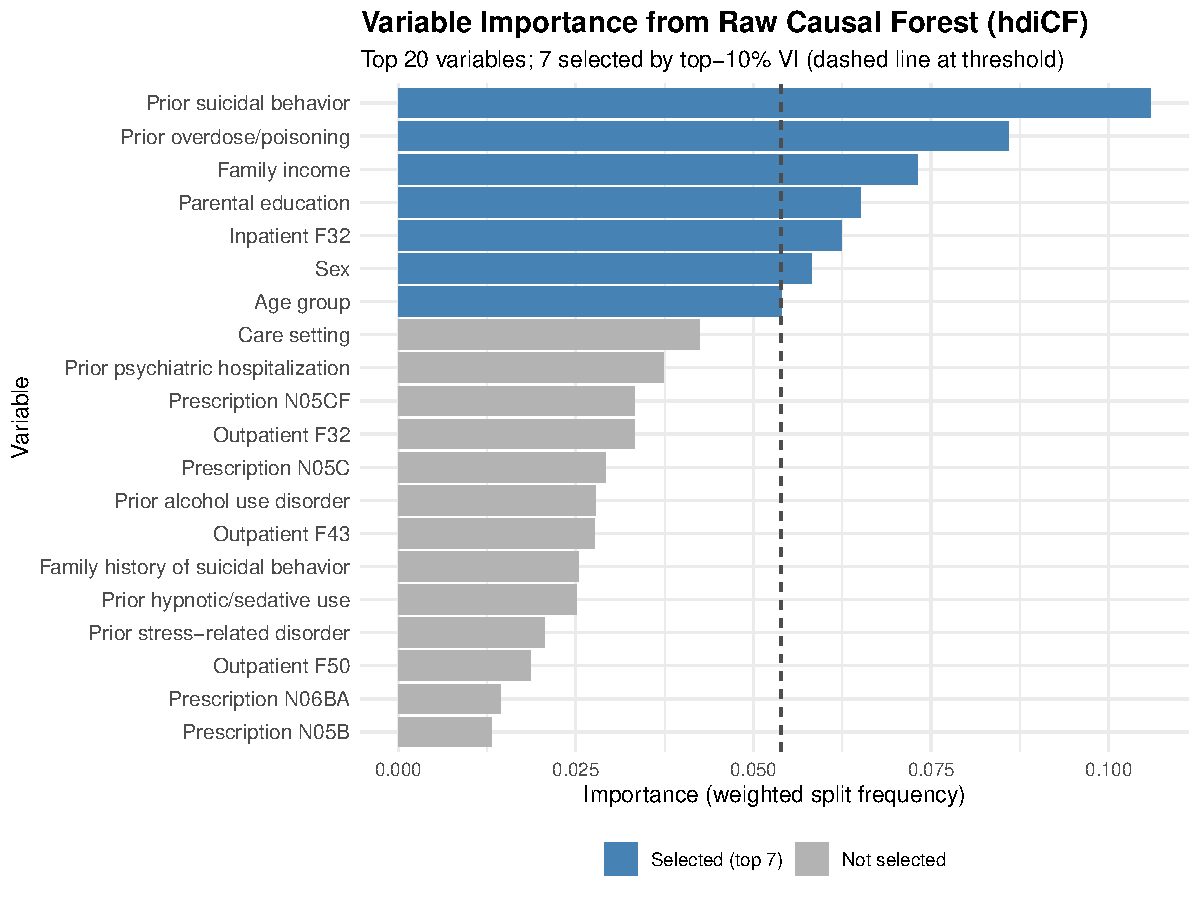
\includegraphics[width=0.9\textwidth]{figures/variable_importance_hdicf.pdf}
\caption{Variable importance from the raw causal forest in the hdiCF pipeline.}
\label{fig:hdicf-varimp}
\end{figure}

The headline tree (Figure~\ref{fig:hdicf-tree}) is the depth-\hdicfBestDepth{} sex split, with stability \hdicfVoteFrequency{} across iCF iterations. Stratified IPW within each leaf reproduces the iCF CATEs to within 0.1~pp, mirroring the base-iCF validation result.

\begin{figure}[H]
\centering
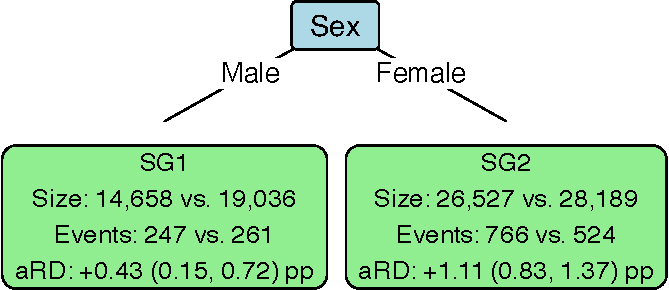
\includegraphics[width=0.5\textwidth]{figures/decision_tree_D2_hdicf.pdf}
\caption{Headline hdiCF decision tree (depth~\protect\hdicfBestDepth, selected by the 1-SE rule).}
\label{fig:hdicf-tree}
\end{figure}

\subsubsection{Per-depth decision trees (hdiCF)}\label{sec:hdicf-per-depth-trees}

As with the base iCF (Section~\ref{sec:icf-per-depth-trees}), we extracted the
voted decision tree at each candidate target depth to examine what additional
structure emerges as the hdiCF tree is allowed to grow deeper.
Figures~\ref{fig:tree-d2-hdicf}--\ref{fig:tree-d5-hdicf} show the four voted
trees.
Target depth~\hdicfBestDepth{}
(Figure~\ref{fig:tree-d2-hdicf}) is the headline while target
depth~\hdicfCVMinDepth{} (Figure~\ref{fig:tree-d4-hdicf}) is the CV-argmin.

\begin{figure}[H]
\centering
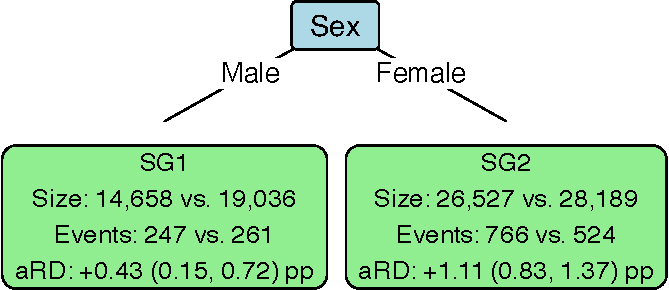
\includegraphics[width=0.6\textwidth]{figures/decision_tree_D2_hdicf.pdf}
\caption{hdiCF voted tree at target depth 2 (\protect\hdicfDTwoNSubgroups{} subgroups).}
\label{fig:tree-d2-hdicf}
\end{figure}

\begin{figure}[H]
\centering
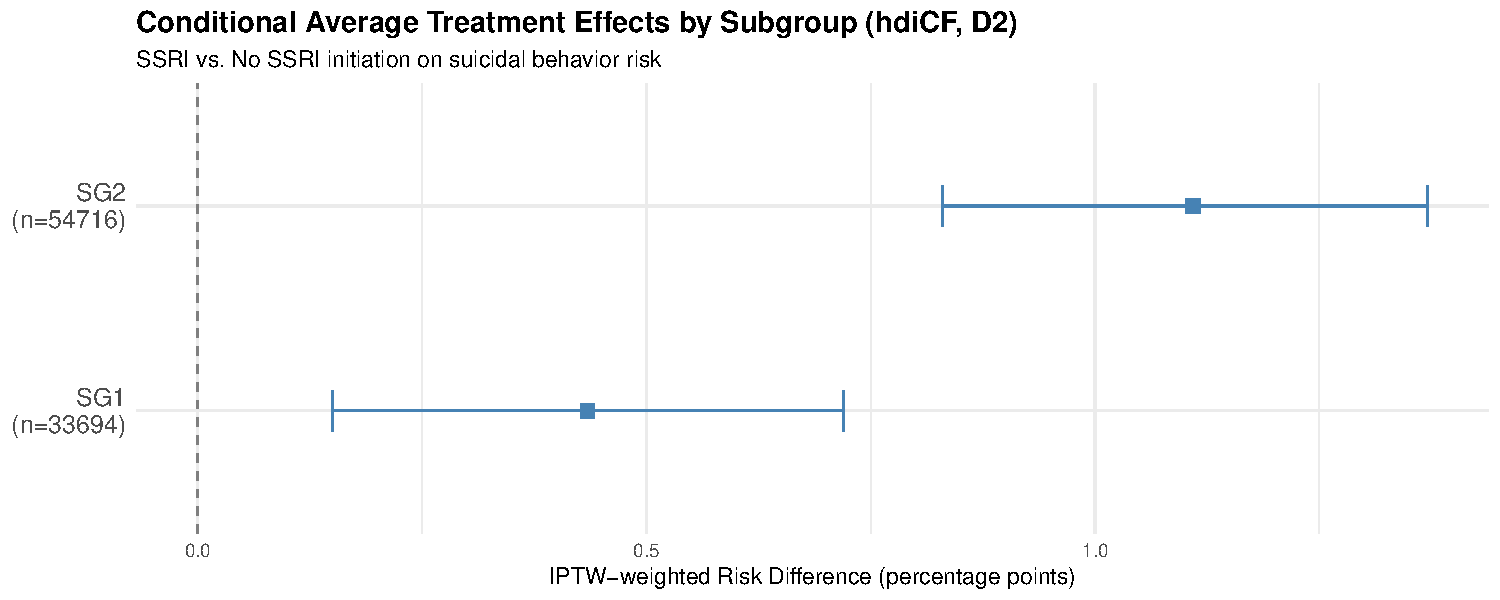
\includegraphics[width=0.9\textwidth]{figures/cate_forest_plot_D2_hdicf.pdf}
\caption{hdiCF subgroup CATEs at target depth 2 (IPTW-weighted risk differences).}
\label{fig:cate-forest-d2-hdicf}
\end{figure}

\begin{figure}[H]
\centering
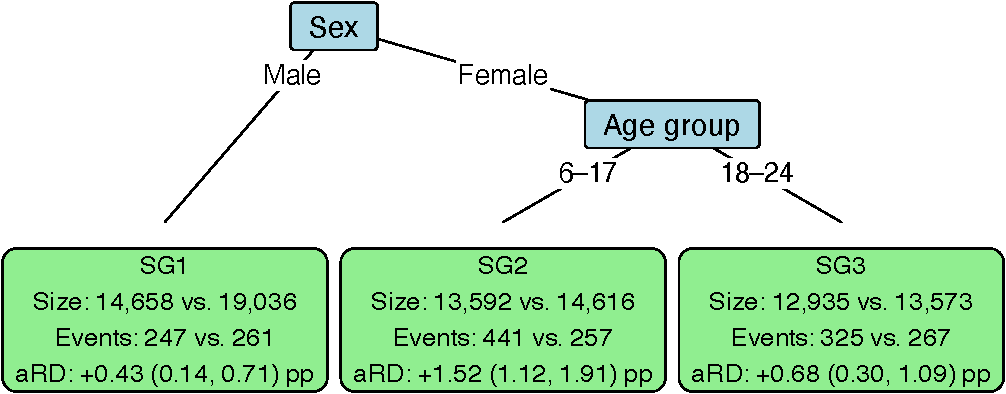
\includegraphics[width=0.8\textwidth]{figures/decision_tree_D3_hdicf.pdf}
\caption{hdiCF voted tree at target depth 3 (\protect\hdicfDThreeNSubgroups{} subgroups).}
\label{fig:tree-d3-hdicf}
\end{figure}

\begin{figure}[H]
\centering
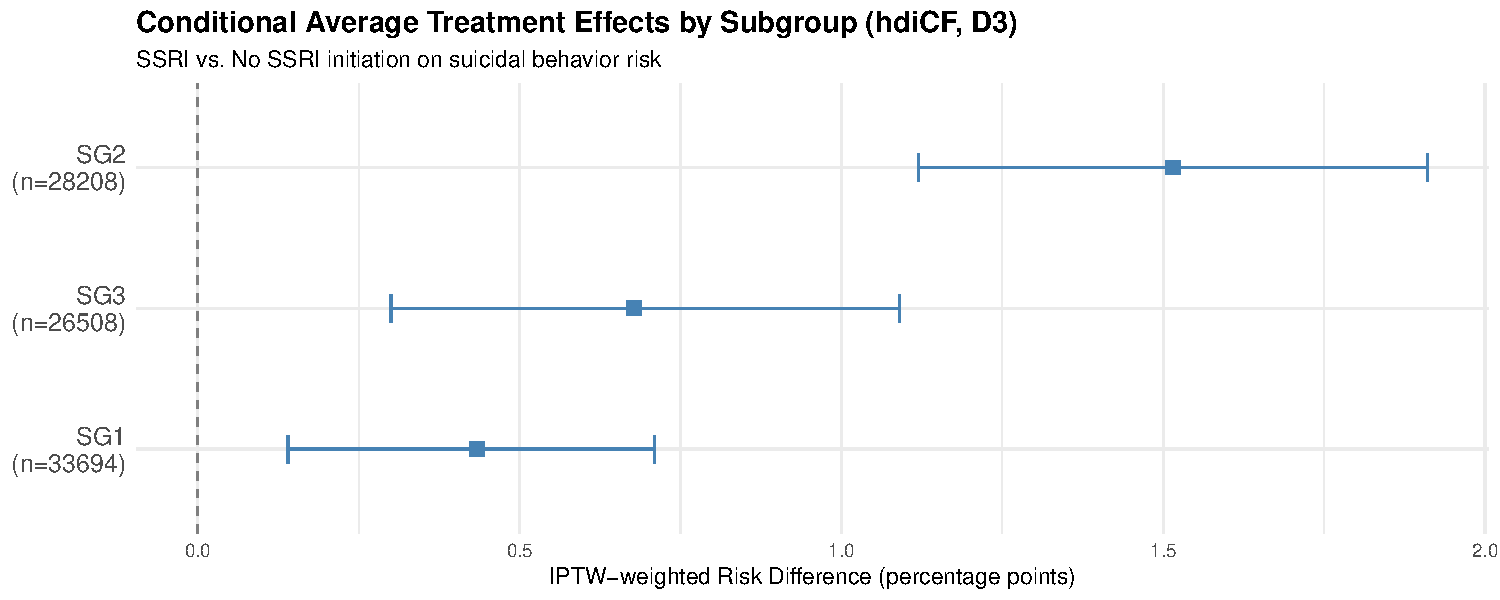
\includegraphics[width=0.9\textwidth]{figures/cate_forest_plot_D3_hdicf.pdf}
\caption{hdiCF subgroup CATEs at target depth 3 (IPTW-weighted risk differences).}
\label{fig:cate-forest-d3-hdicf}
\end{figure}

\begin{figure}[H]
\centering
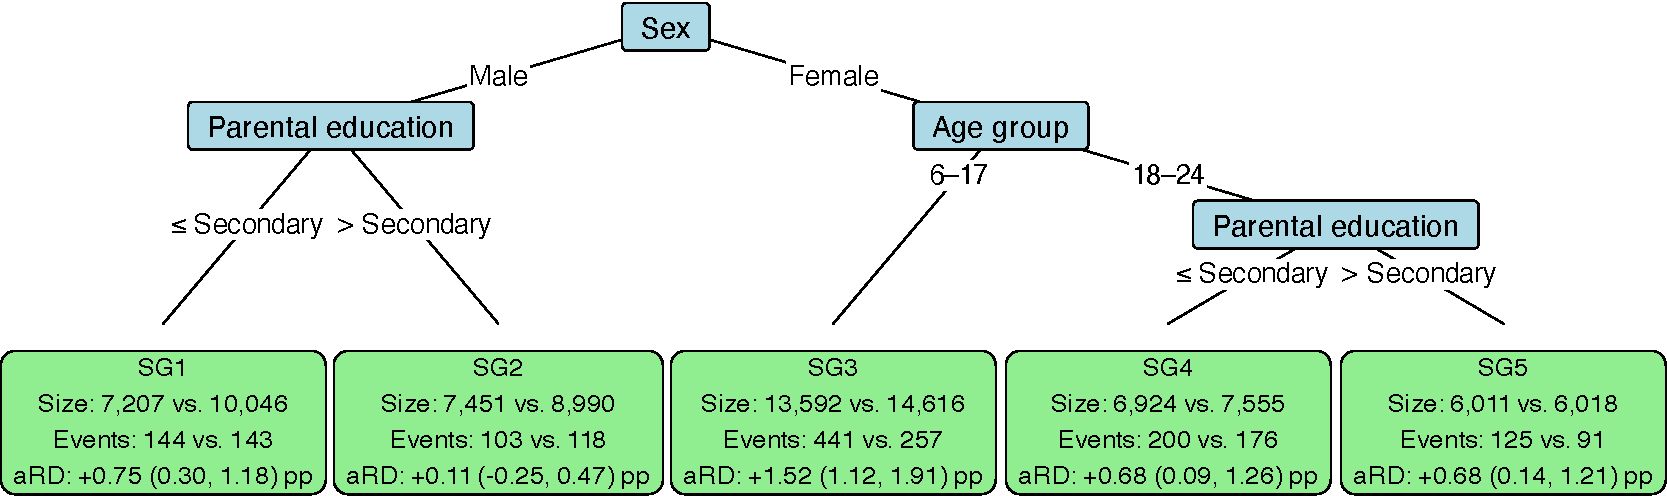
\includegraphics[width=\textwidth]{figures/decision_tree_D4_hdicf.pdf}
\caption{hdiCF voted tree at target depth 4 (\protect\hdicfDFourNSubgroups{} subgroups).}
\label{fig:tree-d4-hdicf}
\end{figure}

\begin{figure}[H]
\centering
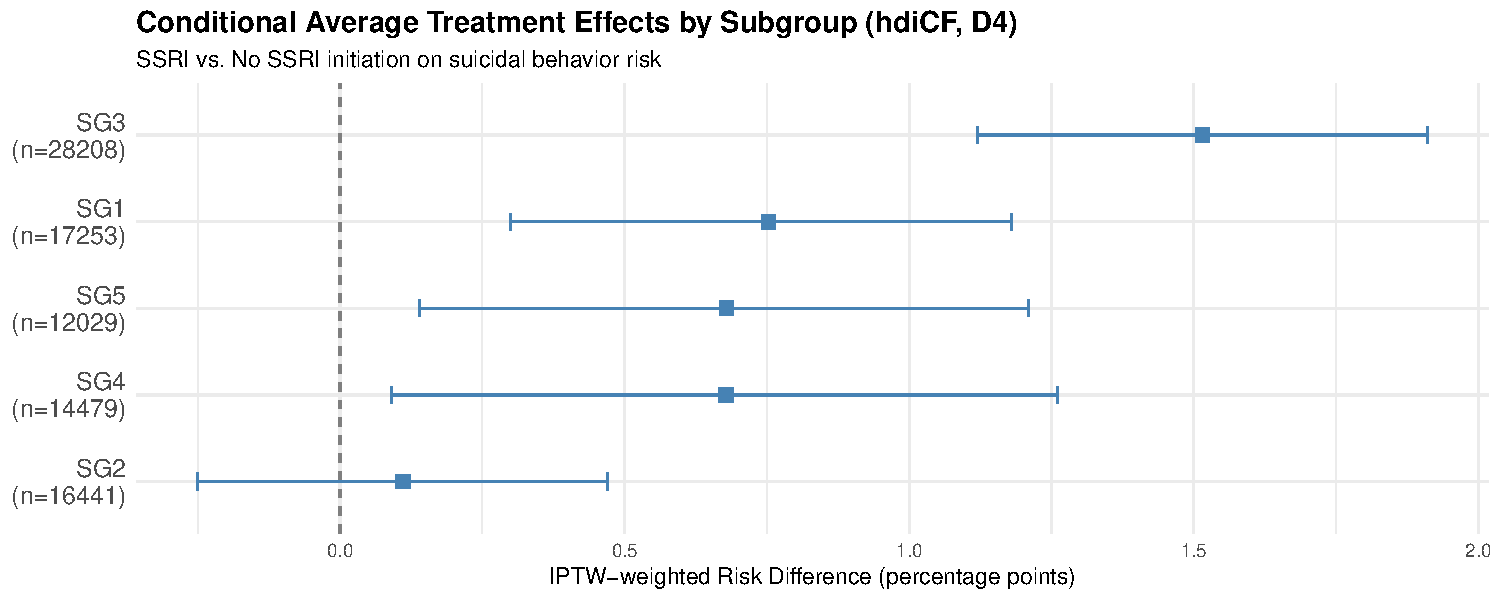
\includegraphics[width=0.9\textwidth]{figures/cate_forest_plot_D4_hdicf.pdf}
\caption{hdiCF subgroup CATEs at target depth 4 (IPTW-weighted risk differences).}
\label{fig:cate-forest-d4-hdicf}
\end{figure}

\begin{figure}[H]
\centering
\makebox[\textwidth][c]{%
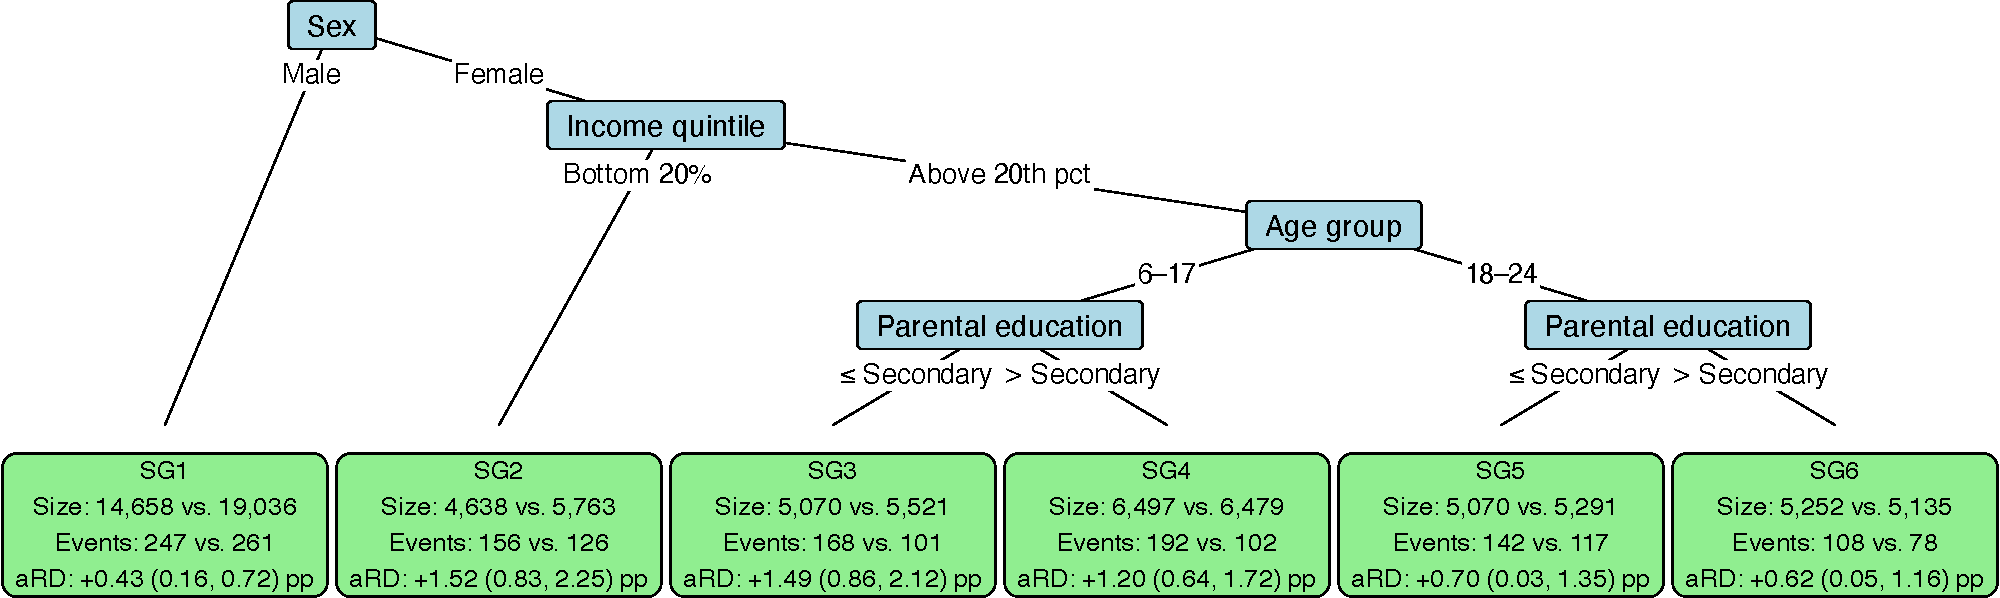
\includegraphics[width=1.2\textwidth]{figures/decision_tree_D5_hdicf.pdf}
}
\caption{hdiCF voted tree at target depth 5 (\protect\hdicfDFiveNSubgroups{} subgroups).}
\label{fig:tree-d5-hdicf}
\end{figure}

\begin{figure}[H]
\centering
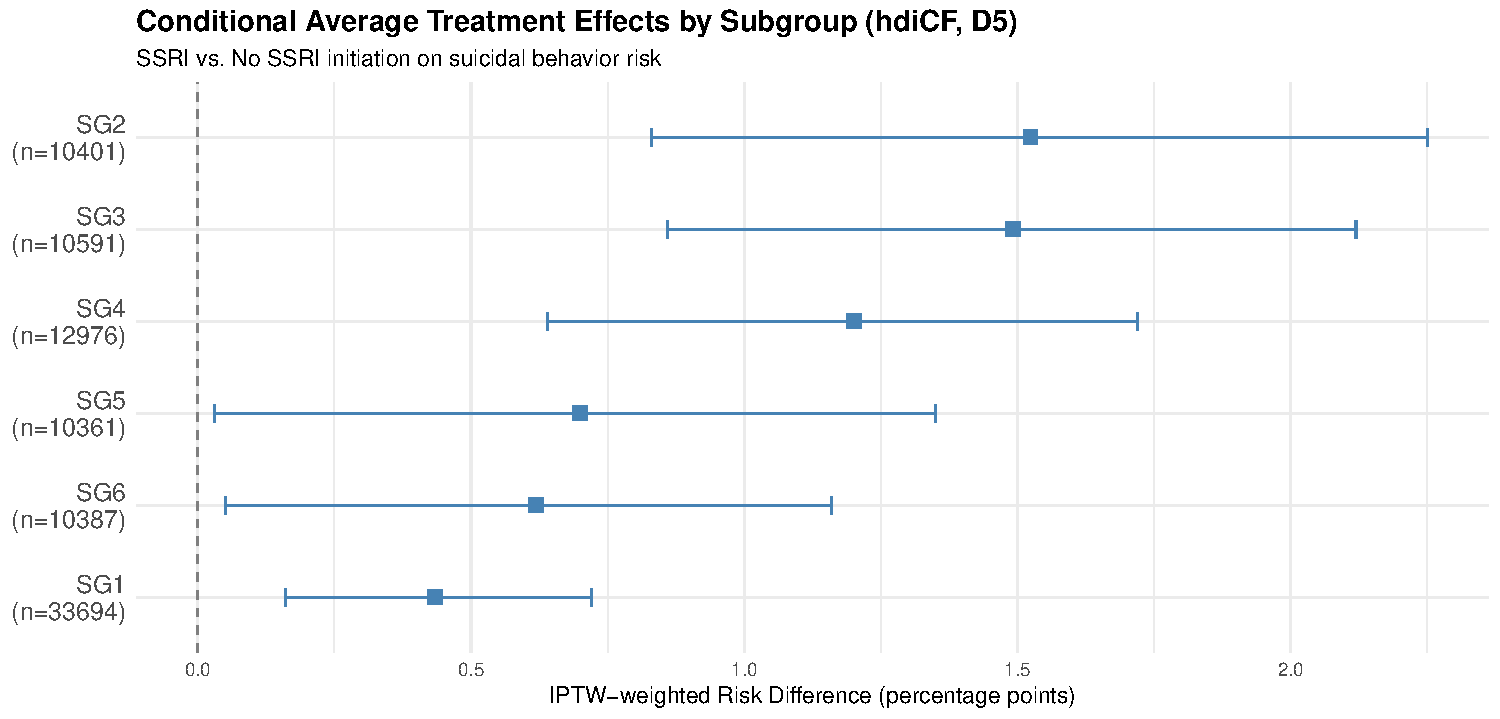
\includegraphics[width=0.9\textwidth]{figures/cate_forest_plot_D5_hdicf.pdf}
\caption{hdiCF subgroup CATEs at target depth 5 (IPTW-weighted risk differences).}
\label{fig:cate-forest-d5-hdicf}
\end{figure}

\subsubsection{Voted-tree structure distribution (hdiCF)}\label{sec:hdicf-structure-dist}

Figure~\ref{fig:structure-dist-hdicf} unpacks the per-depth voted-tree
stability summary in the same way as Figure~\ref{fig:structure-dist} did for
base iCF. At depth~2 the hdiCF iterations converge unanimously on
\texttt{D1:Sex} (\hdicfDTwoNDistinctStruct{} distinct structure).
Depth~3
narrows to \hdicfDThreeNDistinctStruct{} close candidates with the top vote at
\hdicfDThreeVoteFreq{}.
Depth~4 fragments across \hdicfDFourNDistinctStruct{}
distinct structures with the top vote at \hdicfDFourVoteFreq{}.
Depth~5 retains
only \hdicfDFiveNDistinctStruct{} candidate structures and chooses between them
with top vote \hdicfDFiveVoteFreq{}.
Notably, the HD feature (Inpatient F32) does not appear in any of the structures.

\begin{figure}[H]
\centering
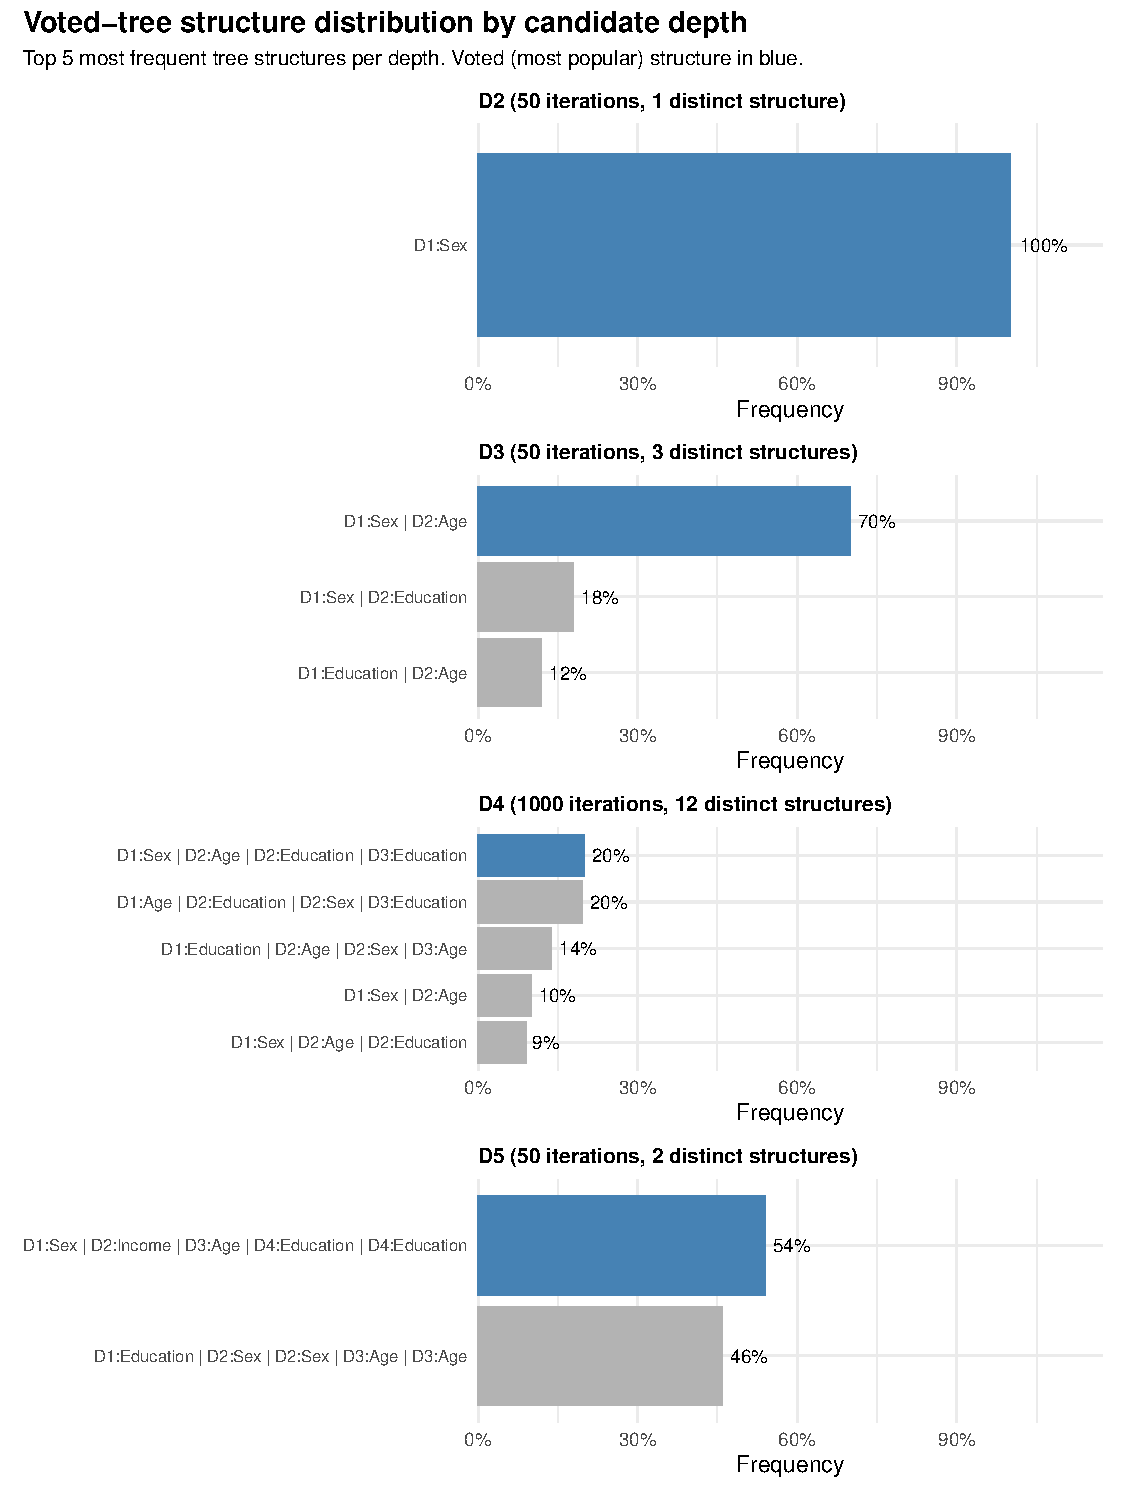
\includegraphics[width=0.95\textwidth]{figures/structure_distribution_hdicf.pdf}
\caption{Voted-tree structure distribution across hdiCF iterations at each candidate depth. Bar length is the fraction of iCF iterations that converged on that structure. The voted (top-plurality) structure is shown in blue. D4 uses 1{,}000 iterations. D2/D3/D5 use 50 iterations each.}
\label{fig:structure-dist-hdicf}
\end{figure}

\subsubsection{Missing-indicator iCF/hdiCF triage}\label{sec:missind-triage}

To rule out that missingness in the four CCA covariates carries detectable
HTE signal the headline iCF and hdiCF are blind to, we reran step~1
(raw causal forest + variable importance) of each pipeline on the full
eligible cohort with a single binary \texttt{any\_miss} indicator added as
a candidate splitting variable (Section~\ref{sec:results-sens-missind}).
The indicator's variable importance was \missindICFAnyMissVI{} in iCF
(mean VI \missindICFMeanVI{}) and \missindHdicfAnyMissVI{} in hdiCF (mean
VI \missindHdicfMeanVI{}). This is well below the above-mean selection
threshold in both pipelines, so \texttt{any\_miss} could not survive variable
selection and could not appear in any voted tree at any depth.

\subsection{Targeting operator characteristic and Qini curves}\label{sec:qini}

To evaluate the clinical value of the causal forest's individual-level CATE
predictions for treatment targeting, we computed Qini curves following
\cite{sverdrup2025}. The Qini curve plots the expected number of suicidal
behavior events that would be prevented by withholding SSRI from the patients
predicted to be most harmed (ranked by CATE), compared to a random withholding
policy. The area under the curve (AUTOC) summarizes the overall gain as a
single number. AUTOC = 0 means CATE-based ranking is no better than random.

\begin{figure}[H]
\centering
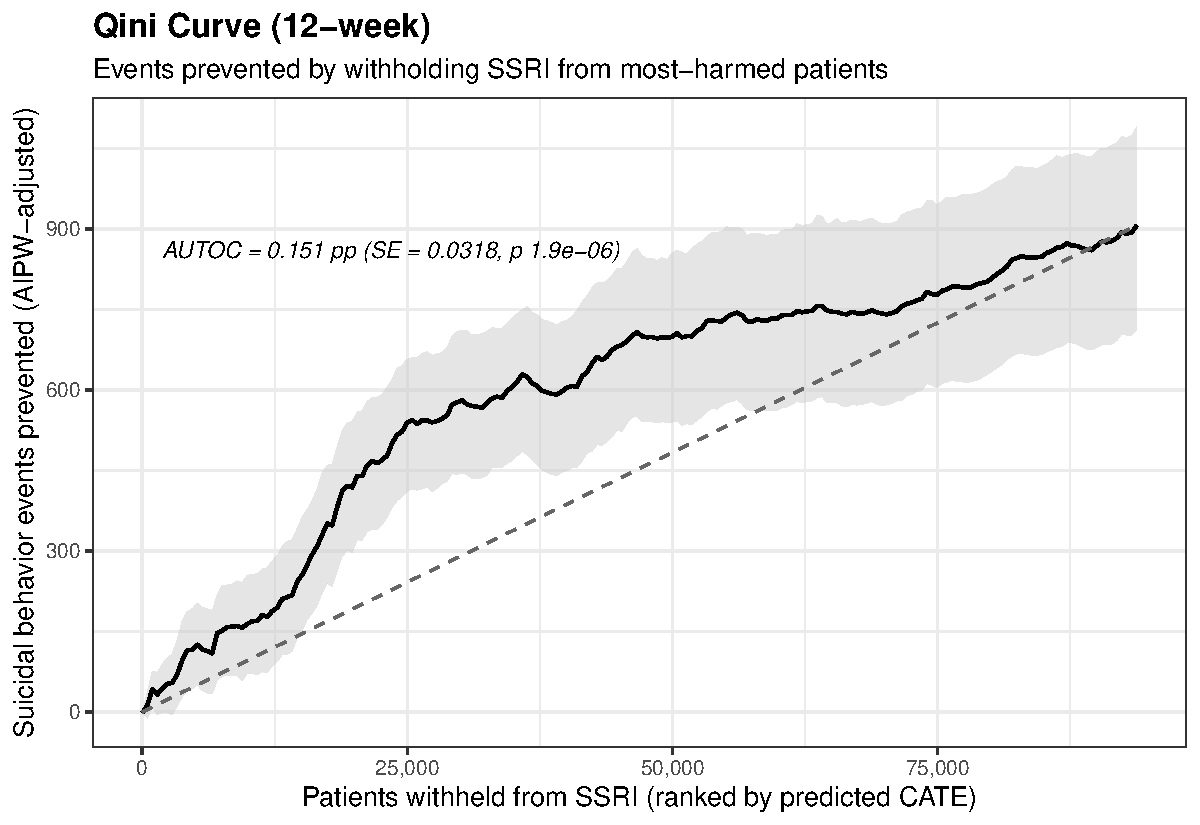
\includegraphics[width=0.9\textwidth]{figures/qini_12wks.pdf}
\caption{Qini curve at 12-week follow-up using individual-level CATE predictions from the base iCF causal forest. Solid line: CATE-based targeting policy. Dashed line: random-policy baseline. Shaded region: 95\% bootstrap CI.}
\label{fig:qini}
\end{figure}

\begin{figure}[H]
\centering
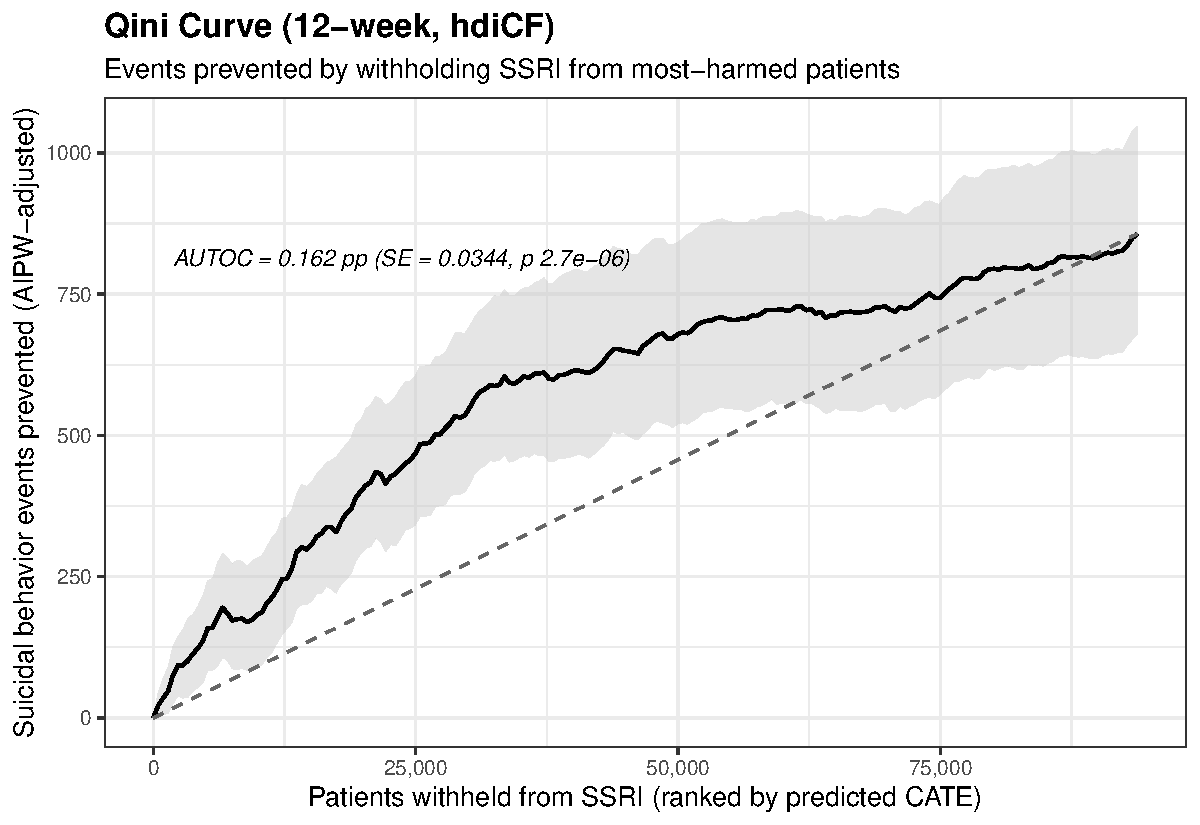
\includegraphics[width=0.9\textwidth]{figures/qini_12wks_hdicf.pdf}
\caption{Qini curve at 12-week follow-up using individual-level CATE predictions from the hdiCF causal forest.}
\label{fig:qini-hdicf}
\end{figure}

The base-iCF AUTOC was \autocTwelve~pp (95\% bootstrap CI \autocTwelveCILower, \autocTwelveCIUpper; $p = \autocTwelvePvalue$).
The hdiCF AUTOC was \autocHdicfTwelve~pp (\autocHdicfTwelveCILower,
\autocHdicfTwelveCIUpper; $p = \autocHdicfTwelvePvalue$). Both AUTOCs are
positive, so per-patient ranking captures some real heterogeneity. Both are
also small relative to the overall ATE (\ittRD~pp), because most of the
heterogeneity is the binary sex contrast that the headline tree already shows.
Hence, ranking patients by predicted CATE adds little on top of just
stratifying by sex.

% ==============================================================================
\section{Discussion}
% ==============================================================================

\subsection{Main analysis}\label{sec:discussion-main}

In a national cohort of \studyN{} Swedish individuals aged 6--24 with a first
depression diagnosis, ITT SSRI initiation within 28 days was estimated to
increase the 12-week absolute risk of suicidal behavior by \ittRD~pp
(95\% CI \ittRDLower, \ittRDUpper), corresponding to a relative risk of
\ittRR{} (\ittRRLower, \ittRRUpper), under the identification assumptions
of the target trial emulation (no unmeasured confounding given the baseline
covariates in Table~\ref{tab:covariates}, positivity, and consistency).
The effect was larger in ages 6--17 (RD \ittYoungRD~pp) than in 18--24 (RD
\ittAdultRD~pp). The headline estimate was robust to excluding inpatient
index diagnoses (\sensExclInpTwelveRD~pp) and to a 14-day grace period
(\sensGraceFourteenTwelveRD~pp).

The closest comparator is Lagerberg et al.\ \cite{lagerberg2023}, a
target-trial emulation of a Stockholm-County cohort (162,267 individuals aged
6--59, depression diagnoses 2006--2018). They reported an overall ITT RD of
0.15~pp (RR 1.50), with age-specific RDs of 1.48~pp (RR 2.90) for ages 6--17
and 0.27~pp (RR 1.59) for ages 18--24, and no effect at age 25+. Our
age-specific estimates match in direction and are broadly comparable in
magnitude. Our larger overall RD (\ittRD~pp vs.\ 0.15~pp) reflects the
cohort restriction to ages 6--24, whereas Lagerberg's overall estimate is
diluted by the much larger and effectively null 25--59 segment.
Methodological differences (national vs.\ Stockholm-only cohort, data
through 2019 vs.\ 2018, Kaplan--Meier with stabilized IPW vs.\ pooled
logistic regression) are unlikely to drive the broad agreement.

The broader RCT evidence is consistent in direction. A meta-analysis of
pediatric antidepressant trials reported roughly a two-fold increase in
suicidal ideation or attempts \citep{bridge2007}, the trigger for the FDA's
2004 black-box warning summarized in \citet{hammad2006}. Our cohort-based
12-week RD falls in the same direction. The main contribution here is
extending the trial-based signal to a population-level emulation under
current real-world prescribing.

\subsection{Subgroup analyses}\label{sec:discussion-subgroups}

\subsubsection{Sex differences}\label{sec:discussion-sex}

The iCF heterogeneity test confirmed that the effect is not
uniform across patients ($p = \icfHetPvalue$).
We found that sex is the main covariate that changes the
SSRI effect.
The 1-SE-selected headline
tree was a single sex split: CATE \icfSGACATE~pp in males
(\icfSGACILower, \icfSGACIUpper) and \icfSGBCATE~pp in females
(\icfSGBCILower, \icfSGBCIUpper), a roughly \icfCATEratio$\times$
difference. We confirmed this in two ways. Firstly, re-estimating each
leaf's effect with a separate method (stratified IPW) reproduced the iCF
CATEs to within 0.1~pp. Secondly, the per-patient targeting analysis (AUTOC =
\autocTwelve~pp, $p = \autocTwelvePvalue$) was positive but small relative
to the overall \ittRD~pp ATE. Hence, the binary sex contrast already captures
most of the heterogeneity, and ranking patients more finely by their
predicted CATE adds little.

The high-dimensional augmentation in hdiCF preserved this sex split
unchanged, with no HD feature stabilizing into any voted tree at any depth.
The implications of this null methodological result for the second research
question are discussed in Section~\ref{sec:discussion-method}.

On the sex axis itself, the most direct comparator is Lagerberg et al.\
\cite{lagerberg2023}'s own sex-stratified analysis (Table~S5),
which we replicate methodologically. Their 12-week per-protocol
results show a substantially elevated risk in females (overall RR 1.91, 95\%
CI 1.23, 2.94; RD 0.23~pp, 95\% CI 0.05, 0.41), concentrated in the 6--17
stratum (RR 4.09, 95\% CI 1.71, 9.80; RD 2.47~pp, 95\% CI 0.19, 4.76, on 84
outcome events). Among males, the overall estimate is
statistically inconclusive (RR 1.38, 95\% CI 0.83, 2.27; RD 0.12~pp, 95\% CI
$-$0.09, 0.33). The corresponding male 6--17 cell is uninformative (only 5
events in initiators; RR CI 0.06, 49.82). Estimates are near-null in both sexes
from age 25 onwards. The directional pattern is consistent with our iCF result:
the effect is larger in females in the pediatric stratum. The male pediatric
CI cautions against reading the male point estimate as definitively null.
Two caveats apply when making a comparison with Lagerberg's results. First,
Lagerberg's sex-stratified analysis is per-protocol whereas our iCF analysis is
based on ITT. Second, they do not report a formal sex--age interaction test.

Beyond the parent paper, evidence on sex-specific effects is sparse. The
FDA's 2004 black-box warning \citep{fda2023prozac} and the pivotal
pediatric meta-analyses \citep{hammad2006, bridge2007} stratified on age,
not on sex, so sex-specific effect modification has not been a headline
finding in that literature. The closest direct comparator is
\citet{termorshuizen2015}, a Dutch retrospective
cohort study (66{,}196 patients starting antidepressants, of whom 5{,}636 were
aged $<$25). This study reported an incidence rate ratio of 1.94 ($p = 0.065$)
for suicide attempts in the first month of treatment among females $<$25,
against 0.52 ($p = 0.368$) in males $<$25, and concluded that female sex was
the modifier of early-attempt risk in young patients. Our analysis is
consistent in direction, our cohort is larger, and we have employed a
target-trial emulation rather than a before-versus-after comparison
window. We therefore place a much sharper estimate around an effect that
Termorshuizen's smaller young-patient subgroup (n = 5{,}636) was
statistically inconclusive about at the conventional 0.05 threshold.

Evidence from RCTs appears to be sparse. \citet{khan2005} pooled 15
placebo-controlled antidepressant trials (323 depressed outpatients, mean age
$\sim$42) and found that the SSRI effect size was roughly twice as large in
women (0.82) as in men (0.44). SSRI responder rates were 64.8\% in women versus
47.5\% in men ($p < 0.05$). It should be noted that the cohort and endpoint are
not the same as ours: Khan studied adults, and the endpoint was symptom
response rather than suicidal behavior. However, the broader pattern emerging
from the RCT-pooled and observational evidence is that sex matters on both
sides of the risk--benefit calculation at SSRI initiation: the female response
appears larger in both the therapeutic and the early-period harm direction. Our
analysis reinforces the harm-side half of that pattern in a population-scale
registry cohort of young people.

\subsubsection{Prior suicidal behavior}\label{sec:discussion-prior-suicidal}

Prior suicidal behavior was the strongest predictor of future suicidal
behavior in this cohort by variable importance
(Figure~\ref{fig:icf-varimp}: importance 0.127, ahead of sex at 0.110).
Despite this,
it never appeared as a split in any voted iCF tree at any candidate depth.
To check whether the iCF voting was missing a real effect modifier, we ran
the IPW-weighted ITT estimate separately within the two prior-suicidality
strata (Section~\ref{sec:strat-prior-suicidal}). The two strata show an
absolute-versus-relative split: patients with a prior suicidal-behavior
diagnosis have a higher baseline risk, a numerically larger
absolute risk increase under SSRI initiation, and a smaller relative risk,
with overlapping 95\% CIs on the RD scale.
Both the stratified estimates and the iCF voting suggest
that prior suicidal
behavior is the strongest prognostic marker in this cohort but does
not detectably modify the SSRI effect on the scale iCF uses to split
(cross-validated MSE of the CATE).
Variable importance in \texttt{grf} counts how often each variable gets
used to split the data across the forest, with splits closer to the root
weighted more heavily because they shape larger parts of the tree. The
algorithm is designed so that these splits are driven by differences
in treatment effect between subgroups, not by who has a higher baseline
outcome risk overall. It achieves this by adjusting both the outcome
and the treatment indicator for the covariates before any split is chosen.
In practice this adjustment is never perfect, and some baseline-risk
signal slips through. As a consequence, a variable can receive a high
importance score either because it genuinely changes how patients respond
to SSRI, or because it strongly predicts who is likely to have the outcome
regardless of treatment. So when a top-ranked variable never appears as a
split in any voted iCF tree, the natural interpretation is that it falls into
the second category: a strong predictor of the outcome, but not an effect
modifier.

Lagerberg et al.\ \cite{lagerberg2023} reported the same null in this
high-risk subgroup (per-protocol RR 1.17, 95\% CI 0.58, 2.34 in patients
with a history of suicidal behavior at baseline; their Table~3). They
noted that the RCT evidence base for this group is thin because patients
with a history of suicidal behavior are routinely excluded from
antidepressant trials. The agreement between our stratified estimate, our
iCF reading, and Lagerberg's own stratified result reinforces a single
conclusion: in a population-scale registry cohort, prior suicidal
behavior identifies the patients at highest baseline risk but does not
appear to alter the direction or magnitude of the SSRI-attributable risk
increase on the relative scale.

\subsubsection{Other subgroupings}\label{sec:discussion-other-subgroups}

The purpose of running iCF and hdiCF was to surface subgroup structure beyond
what pre-specified demographics already capture, so the dominance of sex
deserves a closer look. The variable-importance ranking retained
\icfNSelectedVars{} curated variables (Figure~\ref{fig:icf-varimp}), a
mix of demographics (sex, age group), socioeconomic variables (parental
education, family income), prior-history flags (prior suicidal behavior,
prior overdose, prior psychiatric hospitalization, prior alcohol use), and
family-history indicators. Of these, only sex made it into the headline tree,
and only age appeared as a deeper split the iCF iterations agree on.
The clearest example of the variable-importance-vs-effect-modifier
distinction is prior suicidal behavior, discussed in its own subsection
above (Section~\ref{sec:discussion-prior-suicidal}). The same pattern
holds for prior overdose and prior psychiatric hospitalization: both rank
near the top of the variable-importance ranking but never enter a voted
iCF tree at any candidate depth, suggesting they are prognostic markers
of baseline outcome risk rather than modifiers of the SSRI effect.
``Most important by variable importance'' and ``most important effect
modifier'' are different questions with different answers:
Figure~\ref{fig:icf-varimp} answers the first whereas
Figure~\ref{fig:icf-tree} answers the second.

Across the four candidate tree depths (Section~\ref{sec:icf-per-depth-trees}),
the per-depth voted trees elaborate the headline with age- and SES-based
refinements. The depth-3 tree adds an age split within the female branch
(CATE \icfDThreeSGBCATE~pp at ages 6--17 vs.\ \icfDThreeSGCCATE~pp at ages
18--24, Table~\ref{tab:cv-depth}), matching Lagerberg's age finding
\cite{lagerberg2023}. Deeper trees (D4--D5) add candidate splits on parental
education, family income, and family history. However,
Figure~\ref{fig:structure-dist} shows that the iCF iterations split their
votes across \icfDFourNDistinctStruct{} different D4 tree structures and
\icfDFiveNDistinctStruct{} different D5 structures, with the most-popular
D5 variant promoting age to the root and dropping sex to depth 2. We
therefore read the deeper trees as exploratory rather than confirmed
effect modifiers.
To test whether any of the depth-3+ structures holds up, we would need to apply
this method in a larger cohort where the cross-validated error is not flat
across depth.

\subsubsection{Methodological assessment of (hd)iCF in this cohort}\label{sec:discussion-method}

The second research question asked whether high-dimensional iterative causal
forests can uncover clinically meaningful subgroups in Swedish registry data.
The pipeline did surface the binary sex contrast that replicates across an
independent estimator and aligns with prior evidence
(Section~\ref{sec:discussion-sex}), so the data-driven HTE framework is not
vacuous here. Two findings, however, temper the case for the high-dimensional
augmentation specifically.

First, none of the \hdicfNHDFeatures{} ordinally-encoded ICD-10 and ATC
features generated by hdiCF stabilized into the voted tree at any candidate
depth. The single HD feature that survived the top-10\% importance filter
(inpatient F32) never split a voted tree, and the depth-\hdicfBestDepth{}
headline structure was identical to that of the base iCF
(Section~\ref{sec:hdicf-subgroups}). In this cohort, hdiCF therefore added no
information beyond what the curated covariate set already provided.

Second, the cross-validated MSE landscape was flat across all four candidate
depths (relative range $\sim 10^{-4}$, well below the within-fold SD of
$\sim 10^{-2}$), so the data did not uniquely identify a depth. We fell back
on the CART 1-SE rule to select the shallowest stable structure, but the
iterative procedure's principal selling point --- i.e. letting cross-validation
choose tree depth --- did not discriminate here. The structure-distribution
analysis (Figure~\ref{fig:structure-dist}) shows the same flatness in tree
space. The distribution is unanimous on depth~2 and dispersed across many
roughly-equivalent partitions at depth~4.

The possible explanation is statistical power. With \studyEvents{} events
across \studyN{} patients, the across-depth CV-MSE differences sit well below
within-fold noise. A larger registry cohort, or pooled data across Nordic
registries, would be the natural test of whether hdiCF surfaces additional
structure beyond sex. With the available data, the present analysis cannot
resolve that question.

\subsection{Strengths}

\begin{itemize}
  \item Register infrastructure: Complete national coverage of
        inpatient and outpatient diagnoses (NPR), all dispensed prescriptions
        (PDR), socioeconomic variables (LISA), and pseudonymized parental
        linkages (Multi-Generation Register). This gives us two strengths
        an ordinary clinical trial would not have. First, outcomes are
        captured passively in the registers as long as the patient is alive
        and resident in Sweden, so the cohort has essentially no loss to
        follow-up. Emigration and death are the only ways out and both are
        flagged in the registers. Second, family-history covariates are
        derived from each parent's own NPR record rather than from
        participant self-report, yielding register-based, objective
        family-history measurements that trials almost never have.
  \item Target-trial framework: Explicit alignment of eligibility,
        treatment assignment, and time zero resolves immortal-time bias and
        structures the analysis as a transparent emulation of a hypothetical
        randomized trial \citep{matthews2022, hernan2016}.
  \item Data-driven HTE analysis: The iCF and hdiCF pipelines
        replace the multiplicity of pre-specified subgroup tests with a
        single cross-validated heterogeneity test plus stable
        plurality-voted subgroups, controlling Type I error while still
        letting the data surface effect modifiers
        \citep{sverdrup2025, wang2024icf}.
  \item Validation via independent estimators: Two
        pre-registered sensitivity analyses (inpatient exclusion, 14-day
        grace period) and two independent CATE estimators (IPTW with
        causal-forest propensity scores, stratified logistic-regression IPW)
        provide validation of the headline estimate from
        different statistical methods.
\end{itemize}

\subsection{Limitations}\label{sec:limitations}

\begin{itemize}
  \item Residual confounding: The IPW analysis assumes the
        propensity-score model captures all confounding by indication.
        Depression severity is only crudely proxied by the curated covariates
        (care setting, prior hospitalization, prior anxiety/stress diagnoses).
        We cannot rule out unmeasured confounders such as current suicidal
        ideation, which the NPR captures only when acted upon. The direction of
        any residual bias
        is ambiguous.
  \item Cohort restriction and generalizability: The 12-week follow-up
        window captures the period during which the suicidal-behavior
        signal is strongest in randomized trials but does not characterize
        longer-term effects. The cohort is restricted to patients with a
        first depression diagnosis and no antidepressant in the prior year,
        so the contrast is between starting an SSRI and not starting one.
        Results do not generalize to SSRI use in patients with chronic or
        recurrent treatment histories.
  \item Specialist-care-only cohort: The Swedish National Patient Register
        covers inpatient and specialist-outpatient care but not primary
        care. Depression diagnoses managed entirely in primary care are
        therefore invisible to our cohort. Lagerberg et al.\
        \cite{lagerberg2023} additionally drew on Region Stockholm's VAL
        database, which links primary-care diagnoses and so captures the
        milder cases that never reach specialist care. Our cohort is
        correspondingly biased toward more severe presentations, which may
        make the estimated effects less applicable to the larger segment
        of patients diagnosed and treated entirely in primary care.
  \item Complete-case cohort: Four covariates (parental education, family
        income, family history of depression, family history of suicidal
        behavior) had non-trivial missingness driven by incomplete registry
        coverage rather than by patient or clinician behavior. We
        restricted the analysis cohort to complete cases on these four
        variables, dropping \cohortExcludedCCA{} patients
        (\cohortExcludedCCAPct\% of the post-washout cohort).
        Table~\ref{tab:baseline-excluded} shows that the excluded patients
        differ from the retained cohort on several baseline characteristics,
        so the analysis is clearly not missing completely at random (MCAR).
        This incurs a selection bias.
  \item Missing-indicator bias: The missing-indicator sensitivity analysis
        (Section~\ref{sec:results-sens-missind}) recovers the dropped
        patients and yields essentially the same estimate, but should be
        read as a robustness check rather than an unbiased estimate on the
        full eligible cohort. When the underlying covariate is a confounder,
        the missing-indicator method is known to yield biased treatment-effect
        estimates even under MCAR \citep{groenwold2012missing}, because the
        contrast within the ``missing'' stratum does not correspond to an
        exchangeable comparison.
\end{itemize}

\subsection{Clinical implications}\label{sec:clinical-implications}

The reportable clinical signal is a binary sex difference in early-period
suicidal-behavior risk at SSRI initiation: \icfSGACATE~pp
(\icfSGACILower, \icfSGACIUpper) in males and \icfSGBCATE~pp
(\icfSGBCILower, \icfSGBCIUpper) in females, with the same contrast appearing
at every candidate iCF depth. This adds a sex axis to the FDA black-box
warning's age-only stratification \citep{fda2023prozac} and can reasonably be
raised in a risk discussion at SSRI initiation. The \ittRD~pp overall absolute
increase corresponds to roughly one additional event per hundred patients
treated over 12 weeks. This is small in absolute terms but clinically meaningful
given the severity of the outcome. This risk difference must be balanced against the
unmeasured benefits of SSRI treatment (symptom remission, prevention of
chronic disease). The contrast is between starting an SSRI and not starting
one, not between SSRIs and an active alternative such as psychotherapy.

No subgroup we identified at any depth showed a protective effect of
SSRI initiation on the suicidal-behavior endpoint at 12 weeks. The question
is one of relative magnitude of harm, not of direction. Deeper subgroup
distinctions (age in the female branch at depth 3, income and parental
education at depths 4--5) are hypotheses to be tested against independent
registry data and should not be taken as bases for current prescribing decisions.

\subsection{Future research}

\begin{itemize}
  \item Severity-adjusted re-analysis: A planned follow-up publication will
      re-run the pipeline on a more recent version of the registry data, possibly
        based on the cohort in the Swedish Quality Register for Child and
        Adolescent Psychiatry (QBUP). This would allow the use of the SQD and
        CGAS severity measures for the propensity-score model and the iCF/hdiCF
        feature set.
  \item Replication of deeper iCF structure: Larger cohorts in which
        the CV-MSE landscape is not flat would let the iCF uniquely identify
        a depth and confirm or refute the candidate modifiers (age within
        females, SES gradients) surfaced at depths 3--5.
  \item Independent replication: Other Nordic registries, and
        non-Nordic cohorts with different prescribing patterns, could be used to test
        whether the sex contrast generalizes beyond Sweden.
  \item Longer follow-up: Lagerberg's 52-week curves
        \cite{lagerberg2023} suggest continued accumulation of events beyond
        the 12-week initiation window.
  \item Active comparator: An SSRI vs.\ psychotherapy (or
        watchful-waiting) emulation would address the clinical decision more
        directly than the start-vs-not-start contrast emulated here.
\end{itemize}

% ==============================================================================
\section{Conclusions}
% ==============================================================================

In a national cohort of Swedish youth with a first depression diagnosis, SSRI
initiation within 28 days was estimated to increase the 12-week risk of
suicidal behavior by \ittRD~percentage points (95\% CI \ittRDLower,
\ittRDUpper). The estimate was robust to inpatient-exclusion and 14-day
grace-period sensitivity analyses and broadly aligned with prior
target-trial-emulation evidence in the same age range.
The iCF cross-validated MSE was flat across all candidate depths on this cohort.
After applying the CART 1-SE rule, the data-driven analyses identified
\icfNSubgroups{}
subgroups defined by sex, with the female effect roughly \icfCATEratio$\times$
the male effect. Deeper iCF trees, presented as sensitivity analyses, suggested
further candidate effect modifiers (age, parental education, family income)
that were not stable across iterations and warrant replication in independent
cohorts before they are read as confirmed.
The reproducible signal was a binary
sex difference in early-period suicidal-behavior risk at SSRI initiation.
This identifies sex as a candidate axis of caution to weigh in the
risk-benefit discussion at SSRI initiation, beyond the age-based
stratification of the FDA's existing pediatric black-box warning.

\section*{Declaration of AI use}
\addcontentsline{toc}{section}{Declaration of AI use}

I used Claude Code and OpenAI ChatGPT to assist in:

\begin{itemize}
    \item Converting the original SAS data extraction scripts into R,
    \item Implementing the data extraction and analysis pipelines,
    \item Checking for bugs in the implementation,
    \item Interpreting the results and generating ideas on how to improve them,
    \item Checking for errors in the written report.
\end{itemize}

% ==============================================================================
% References
% ==============================================================================
\newpage
\bibliographystyle{unsrtnat}
\bibliography{references}

% ==============================================================================
% Appendix
% ==============================================================================
\newpage
\appendix

\section{Supplementary tables}

\subsection{Variable name mapping}

Table~\ref{tab:varname-mapping} maps the raw variable names used in the analysis code (e.g., R script outputs, log files, intermediate RDS files) to the human-readable labels used in the body of this report.

{\setlength{\tabcolsep}{4pt}
\renewcommand{\arraystretch}{0.95}
\begin{longtable}{lp{\dimexpr 0.55\textwidth-2\tabcolsep}}
\caption{Mapping between raw variable names and human-readable labels} \label{tab:varname-mapping} \\
\toprule
\textbf{Raw name} & \textbf{Human-readable label} \\
\midrule
\endfirsthead
\multicolumn{2}{l}{\itshape (Table~\ref{tab:varname-mapping} continued)} \\
\toprule
\textbf{Raw name} & \textbf{Human-readable label} \\
\midrule
\endhead
\midrule
\multicolumn{2}{r}{\itshape (continued on next page)} \\
\endfoot
\bottomrule
\endlastfoot
\multicolumn{2}{l}{\textit{Treatment and outcome}} \\
\quad \texttt{cc} & SSRI initiation indicator \\
\quad \texttt{sb12\_itt} & Suicidal behavior outcome (12-week ITT) \\
\quad \texttt{fu\_start} & Index date / time zero / baseline \\
\quad \texttt{fu\_end\_itt} & End of ITT follow-up (event, death, emigration, or week 12) \\
\quad \texttt{diagn\_date} & Date of first recorded depression diagnosis \\
\addlinespace
\multicolumn{2}{l}{\textit{Demographics and SES}} \\
\quad \texttt{female} & Sex \\
\quad \texttt{age} & Age \\
\quad \texttt{age\_cat} & Age category \\
\quad \texttt{year} & Calendar year \\
\quad \texttt{source} & Care setting \\
\quad \texttt{edufam\_cat} & Parental education \\
\quad \texttt{inc\_cat} & Family income \\
\addlinespace
\multicolumn{2}{l}{\textit{Family history}} \\
\quad \texttt{fh\_suicidal} & Family history of suicidal behavior (count of biological parents) \\
\quad \texttt{fh\_depr} & Family history of depression (count of biological parents) \\
\addlinespace
\multicolumn{2}{l}{\textit{Prior psychiatric diagnoses}} \\
\quad \texttt{diag\_organic} & Organic mental disorder \\
\quad \texttt{diag\_alcohol} & Alcohol use disorder \\
\quad \texttt{diag\_sud} & Substance use disorder \\
\quad \texttt{diag\_psychotic} & Psychotic disorder \\
\quad \texttt{diag\_bipolar} & Bipolar disorder \\
\quad \texttt{diag\_mdd} & Major depressive disorder (not used as covariate; constant=1) \\
\quad \texttt{diag\_phobic} & Phobic anxiety disorder \\
\quad \texttt{diag\_anxiety\_other} & Other anxiety disorder \\
\quad \texttt{diag\_anxiety} & Combined F40+F41 anxiety indicator \\
\quad \texttt{diag\_ocd} & Obsessive-compulsive disorder \\
\quad \texttt{diag\_stress} & Stress/adjustment disorder \\
\quad \texttt{diag\_anorexia} & Anorexia nervosa \\
\quad \texttt{diag\_bulimia} & Bulimia nervosa \\
\quad \texttt{diag\_sleep} & Sleep disorder \\
\quad \texttt{diag\_personality\_cluster\_b} & Cluster B personality disorder \\
\quad \texttt{diag\_intellectual\_disability} & Intellectual disability \\
\quad \texttt{diag\_autism} & Autism spectrum disorder \\
\quad \texttt{diag\_adhd} & ADHD \\
\quad \texttt{diag\_conduct} & Conduct disorder \\
\quad \texttt{diag\_overdose} & Overdose/poisoning \\
\quad \texttt{diag\_suicidal} & Prior suicidal behavior \\
\addlinespace
\multicolumn{2}{l}{\textit{Prior medications (within 90 days before baseline)}} \\
\quad \texttt{med\_antipsychotic} & Antipsychotic \\
\quad \texttt{med\_hypnotic} & Hypnotic/sedative \\
\quad \texttt{med\_benzodiazepine} & Benzodiazepine \\
\quad \texttt{med\_antiepileptic} & Antiepileptic \\
\quad \texttt{med\_mood\_stabilizer} & Mood stabilizer \\
\quad \texttt{med\_stimulant} & Psychostimulant \\
\quad \texttt{med\_opioid} & Opioid \\
\quad \texttt{med\_addiction} & Addiction medication \\
\addlinespace
\multicolumn{2}{l}{\textit{Healthcare utilization}} \\
\quad \texttt{hosp} & Prior psychiatric hospitalization \\
\addlinespace
\multicolumn{2}{l}{\textit{HD features (hdiCF only)}} \\
\quad \texttt{dx.inp.<code>} & Inpatient ICD-10 3-character code (e.g., \texttt{dx.inp.F32}) \\
\quad \texttt{dx.out.<code>} & Outpatient ICD-10 3-character code (e.g., \texttt{dx.out.F40}) \\
\quad \texttt{rx.<code>} & ATC 5-character chemical-subgroup code dispensed within 90 days (e.g., \texttt{rx.N05BA}) \\
\end{longtable}
}

\subsection{Missingness patterns in the four CCA covariates}\label{sec:missingness-patterns}

The complete-case analysis cohort (Section~\ref{sec:covariates-complete-case})
excludes patients with any missing value in the four partially-observed
covariates: parental education, family income, family history of suicidal
behavior, and family history of depression. Across the \studyNEligible{}
patients in the pre-CCA eligible cohort, only 5 of the $2^4 = 16$ possible
missingness patterns are observed (Table~\ref{tab:missingness-patterns}). The
remaining 11 patterns are empty.

\begin{table}[H]
\centering
\caption[Missingness patterns across the four CCA covariates]{Missingness patterns across the four partially-observed covariates that drive the complete-case analysis cohort. PE = parental education; FI = family income; FH-S = family history of suicidal behavior; FH-D = family history of depression. $\checkmark$ = observed; $\times$ = missing. Percentages are out of the pre-CCA eligible cohort (N = \studyNEligible). Patterns with zero patients are omitted.}
\label{tab:missingness-patterns}
\begin{tabular}{lccccrr}
\toprule
\textbf{Pattern} & \textbf{PE} & \textbf{FI} & \textbf{FH-S} & \textbf{FH-D} & \textbf{N} & \textbf{\%} \\
\midrule
None missing & $\checkmark$ & $\checkmark$ & $\checkmark$ & $\checkmark$ & 88,427 & 94.28 \\
Family income missing & $\checkmark$ & $\times$ & $\checkmark$ & $\checkmark$ & 953 & 1.02 \\
Parental education missing & $\times$ & $\checkmark$ & $\checkmark$ & $\checkmark$ & 218 & 0.23 \\
Parental education + family income missing & $\times$ & $\times$ & $\checkmark$ & $\checkmark$ & 274 & 0.29 \\
All four missing & $\times$ & $\times$ & $\times$ & $\times$ & 3,923 & 4.18 \\
\bottomrule

\end{tabular}
\end{table}

\subsection{Baseline characteristics of patients excluded by the complete-case restriction}\label{sec:baseline-excluded}

Table~\ref{tab:baseline-excluded} compares the \cohortExcludedCCA{} patients dropped by the complete-case restriction against the \studyN{} patients retained in the analysis cohort, on demographics, the index-diagnosis care setting, the four partially-observed covariates, and two outcome-adjacent prior diagnoses. The SMD column quantifies the magnitude of any systematic difference between the excluded and the included groups on each variable.

{\setlength{\tabcolsep}{4pt}
\renewcommand{\arraystretch}{0.95}
\begin{longtable}{lccc}
\caption[Baseline characteristics of patients excluded by the complete-case restriction]{Baseline characteristics of the \cohortExcludedCCA{} patients excluded by the complete-case restriction (Excluded column) compared to the \studyN{} patients retained in the analysis cohort (Included column). SMD = absolute standardized mean difference between the two groups. Values $>$0.1 indicate notable imbalance.} \label{tab:baseline-excluded} \\
\toprule
\textbf{Characteristic} & \textbf{Excluded} & \textbf{Included} & \textbf{SMD} \\
 & (N = \cohortExcludedCCA) & (N = \studyN) & \\
\midrule
\endfirsthead
\multicolumn{4}{l}{\itshape (Table~\ref{tab:baseline-excluded} continued)} \\
\toprule
\textbf{Characteristic} & \textbf{Excluded} & \textbf{Included} & \textbf{SMD} \\
 & (N = \cohortExcludedCCA) & (N = \studyN) & \\
\midrule
\endhead
\midrule
\multicolumn{4}{r}{\itshape (continued on next page)} \\
\endfoot
\bottomrule
\endlastfoot
% Auto-generated by Summary_statistics.R -- do not edit manually
% Generated: 2026-05-14 16:51:47.645108
\textit{Demographics} &  &  &  \\
\quad Female, n (\%) & 2,679 (49.9) & 54,730 (61.9) & 0.24 \\
\quad Age category (years) &  &  & 0.29 \\
\quad\quad 6--11 & 73 (1.4) & 2,288 (2.6) &  \\
\quad\quad 12--17 & 1,730 (32.2) & 39,919 (45.1) &  \\
\quad\quad 18--24 & 3,565 (66.4) & 46,220 (52.3) &  \\
\textit{Source of depression diagnosis} &  &  &  \\
\quad Care setting &  &  & 0.19 \\
\quad\quad Outpatient & 4,492 (83.7) & 79,612 (90.0) &  \\
\quad\quad Inpatient & 821 (15.3) & 8,440 (9.5) &  \\
\quad\quad Other/unknown source & 55 (1.0) & 375 (0.4) &  \\
\textit{Partially-observed covariates} &  &  &  \\
\quad Parental education &  &  & 3.20 \\
\quad\quad Primary & 244 (4.5) & 4,842 (5.5) &  \\
\quad\quad Secondary & 408 (7.6) & 40,678 (46.0) &  \\
\quad\quad Post-secondary & 301 (5.6) & 42,907 (48.5) &  \\
\quad\quad Missing & 4,415 (82.2) & 0 (0.0) &  \\
\quad Family income &  &  & 7.16 \\
\quad\quad Negative & 2 (0.0) & 167 (0.2) &  \\
\quad\quad Zero & 15 (0.3) & 137 (0.2) &  \\
\quad\quad 1st--20th percentile & 115 (2.1) & 16,625 (18.8) &  \\
\quad\quad 20th--80th percentile & 81 (1.5) & 53,650 (60.7) &  \\
\quad\quad $>$80th percentile & 5 (0.1) & 17,848 (20.2) &  \\
\quad\quad Missing & 5,150 (95.9) & 0 (0.0) &  \\
\quad Family history of suicidal behavior &  &  & 2.33 \\
\quad\quad Neither parent & 1,351 (25.2) & 79,633 (90.1) &  \\
\quad\quad One parent & 89 (1.7) & 8,347 (9.4) &  \\
\quad\quad Both parents & 5 (0.1) & 447 (0.5) &  \\
\quad\quad Missing & 3,923 (73.1) & 0 (0.0) &  \\
\quad Family history of depression &  &  & 2.36 \\
\quad\quad Neither parent & 1,243 (23.2) & 65,675 (74.3) &  \\
\quad\quad One parent & 194 (3.6) & 20,576 (23.3) &  \\
\quad\quad Both parents & 8 (0.1) & 2,176 (2.5) &  \\
\quad\quad Missing & 3,923 (73.1) & 0 (0.0) &  \\
\textit{Outcome-adjacent prior diagnoses} &  &  &  \\
\quad Prior suicidal behavior, n (\%) & 555 (10.3) & 7,539 (8.5) & 0.06 \\
\quad Overdose/poisoning, n (\%) & 432 (8.0) & 5,927 (6.7) & 0.05 \\

\end{longtable}
}

\subsection{High-dimensional features for hdiCF}

Table~\ref{tab:hd-features} lists the \hdicfNHDFeatures{} automatically generated high-dimensional features used by the hdiCF pipeline, grouped by source and ordered by population prevalence within each group. Inpatient and outpatient diagnoses are 3-character ICD-10 codes recorded on or before the index date. Prescription features are 5-character (chemical-subgroup) ATC codes dispensed in the 90 days up to and including the index date, with antidepressants (N06A) excluded by construction (Section~\ref{sec:hte-methods}). Codes with prevalence below 1\% were filtered out during feature generation.

{\setlength{\tabcolsep}{4pt}
\renewcommand{\arraystretch}{0.95}
\begin{longtable}{lp{8cm}r}
\caption{Generated high-dimensional features used by hdiCF, with population prevalence (\%).} \label{tab:hd-features} \\
\toprule
\textbf{Feature} & \textbf{Description} & \textbf{Prevalence (\%)} \\
\midrule
\endfirsthead
\multicolumn{3}{l}{\itshape (Table~\ref{tab:hd-features} continued)} \\
\toprule
\textbf{Feature} & \textbf{Description} & \textbf{Prevalence (\%)} \\
\midrule
\endhead
\midrule
\multicolumn{3}{r}{\itshape (continued on next page)} \\
\endfoot
\bottomrule
\endlastfoot
% Auto-generated by 06_export_hd_features_table.R -- do not edit manually
\textit{Inpatient ICD-10} & & \\
\quad \texttt{dx.inp.F32} & Depressive episode & 11.96 \\
\quad \texttt{dx.inp.F10} & Alcohol use disorder & 3.53 \\
\quad \texttt{dx.inp.X64} & Intentional self-poisoning by drugs (NOS) & 3.20 \\
\quad \texttt{dx.inp.T50} & Poisoning by drugs and biological substances & 3.04 \\
\quad \texttt{dx.inp.F43} & Reaction to severe stress / adjustment disorder & 2.90 \\
\quad \texttt{dx.inp.F90} & Hyperkinetic disorder (ADHD) & 2.25 \\
\quad \texttt{dx.inp.F19} & Multiple substance use disorder & 1.50 \\
\quad \texttt{dx.inp.F50} & Eating disorder & 1.36 \\
\quad \texttt{dx.inp.F84} & Autism spectrum disorder & 1.00 \\
\addlinespace
\textit{Outpatient ICD-10} & & \\
\quad \texttt{dx.out.F32} & Depressive episode & 84.88 \\
\quad \texttt{dx.out.F90} & Hyperkinetic disorder (ADHD) & 13.44 \\
\quad \texttt{dx.out.F33} & Recurrent depressive disorder & 9.18 \\
\quad \texttt{dx.out.F43} & Reaction to severe stress / adjustment disorder & 8.63 \\
\quad \texttt{dx.out.F50} & Eating disorder & 6.94 \\
\quad \texttt{dx.out.F41} & Other anxiety disorder & 5.71 \\
\quad \texttt{dx.out.F84} & Autism spectrum disorder & 5.26 \\
\quad \texttt{dx.out.F40} & Phobic anxiety disorder & 4.37 \\
\quad \texttt{dx.out.F98} & Other behavioural / emotional disorder of childhood & 3.75 \\
\quad \texttt{dx.out.F51} & Non-organic sleep disorder & 3.66 \\
\quad \texttt{dx.out.F10} & Alcohol use disorder & 3.59 \\
\quad \texttt{dx.out.F42} & Obsessive--compulsive disorder & 2.56 \\
\quad \texttt{dx.out.F12} & Cannabinoid use disorder & 1.89 \\
\quad \texttt{dx.out.F19} & Multiple substance use disorder & 1.84 \\
\quad \texttt{dx.out.F91} & Conduct disorder & 1.77 \\
\quad \texttt{dx.out.T50} & Poisoning by drugs and biological substances & 1.55 \\
\quad \texttt{dx.out.F60} & Specific personality disorder & 1.52 \\
\quad \texttt{dx.out.X64} & Intentional self-poisoning by drugs (NOS) & 1.51 \\
\quad \texttt{dx.out.X78} & Intentional self-harm by sharp object & 1.11 \\
\quad \texttt{dx.out.F31} & Bipolar affective disorder & 1.08 \\
\quad \texttt{dx.out.F70} & Mild intellectual disability & 1.05 \\
\addlinespace
\textit{ATC (90 days before baseline)} & & \\
\quad \texttt{rx.N05B} & Anxiolytics & 16.73 \\
\quad \texttt{rx.N05CH} & Melatonin receptor agonists & 10.00 \\
\quad \texttt{rx.N05C} & Hypnotics and sedatives & 6.41 \\
\quad \texttt{rx.N06BA} & Centrally acting sympathomimetics (ADHD stimulants) & 6.10 \\
\quad \texttt{rx.N05CF} & Benzodiazepine-related hypnotics (Z-drugs) & 5.74 \\
\quad \texttt{rx.N05BA} & Benzodiazepine anxiolytics & 3.03 \\
\quad \texttt{rx.N05AH} & Atypical antipsychotics (diazepines / thiazepines) & 1.94 \\
\quad \texttt{rx.N03AX} & Other antiepileptics & 1.21 \\
\quad \texttt{rx.N05AX} & Other antipsychotics & 1.08 \\

\end{longtable}
}

\subsection{Auto-tuner instability of the raw causal forest}\label{sec:tuner-instability}

Section~\ref{sec:hte-methods} reports that the raw causal forest used for
variable selection is grown with \texttt{tune.parameters = "none"} because the
\texttt{grf} auto-tuner picks essentially at random across RNG seeds on this
cohort. Table~\ref{tab:tuner-instability} provides the underlying evidence:
five raw-CF fits to the same data (N = 88{,}427, 36 candidate covariates),
using the same code path as the production pipeline but with
\texttt{tune.parameters = "all"} and seeds $\{42, 43, 44, 45, 46\}$, each
producing its own tuner-selected configuration and downstream above-mean
variable-importance selection set.

\begin{table}[H]
\centering
\caption[Hyperparameters chosen by \texttt{grf}'s auto-tuner across five RNG seeds]{Hyperparameters chosen by \texttt{grf}'s auto-tuner across five RNG seeds for the raw causal forest used in iCF variable selection. Each column is one fit to the same data under \texttt{tune.parameters = "all"}. The bottom row is the size of the above-mean variable-importance selection set that would be passed to the iCF iterative stage. The selection set ranges from 4 to 14 variables, all at essentially identical CV fit (relative range of CV-MSE across seeds $\sim 10^{-4}$).}
\label{tab:tuner-instability}
\begin{tabular}{lrrrrr}
\toprule
\textbf{Hyperparameter} & \textbf{Seed 42} & \textbf{Seed 43} & \textbf{Seed 44} & \textbf{Seed 45} & \textbf{Seed 46} \\
\midrule
\texttt{sample.fraction}      & 0.462 & 0.433 & 0.300 & 0.325 & 0.061 \\
\texttt{mtry}                 & 17    & 21    & 19    & 14    & 10    \\
\texttt{min.node.size}        & 70    & 38    & 561   & 106   & 472   \\
\texttt{honesty.fraction}     & 0.557 & 0.686 & 0.649 & 0.727 & 0.686 \\
\texttt{honesty.prune.leaves} & 0     & 1     & 1     & 1     & 0     \\
\texttt{alpha}                & 0.014 & 0.099 & 0.018 & 0.008 & 0.172 \\
\texttt{imbalance.penalty}    & 1.119 & 1.472 & 0.405 & 0.837 & 0.292 \\
\midrule
Above-mean selection-set size & 13    & 9     & 12    & 14    & 4     \\
\bottomrule
\end{tabular}
\end{table}

The most extreme draw (seed 46, \texttt{sample.fraction} = 0.06) is an
aggressive-shrinkage configuration in which 32 of the 36 candidate covariates
received zero variable importance. In contrast, seed 45 retained 14 variables
above the importance mean. Disabling the auto-tuner and fixing \texttt{seed =
42L} eliminates this source of nondeterminism: two consecutive runs of the
production pipeline produce byte-identical variable importance.

\section{Supplementary figures}

\begin{figure}[H]
\centering
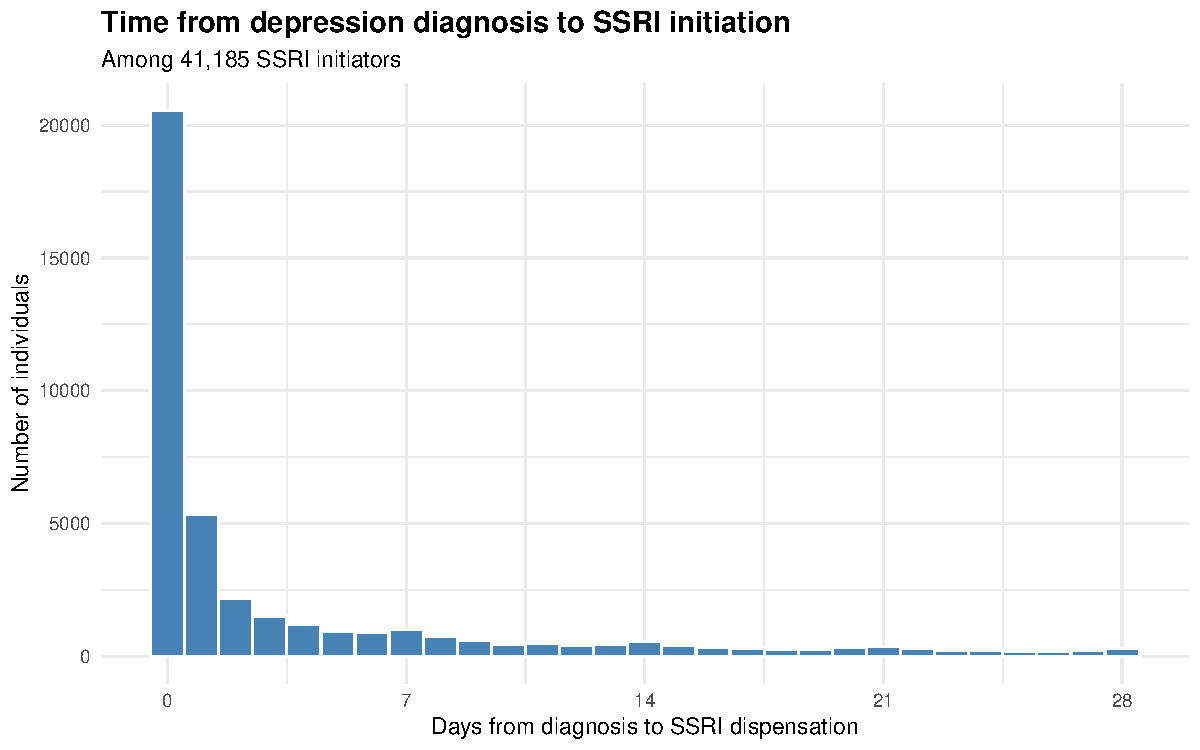
\includegraphics[width=0.9\textwidth]{figures/predi_diff_distribution.pdf}
\caption{Distribution of time from depression diagnosis to SSRI dispensation among the \studyNInitiators{} initiators in the complete-case analysis cohort (same denominator as Table~\ref{tab:baseline}). Approximately half initiated SSRI on the same day as their diagnosis (day 0). The 28-day grace period captures the vast majority of initiations, with a steep drop-off after the first week.}
\label{fig:predi-diff}
\end{figure}

\end{document}
